% Chapter 1

\chapter{Results: Wind turbine array} % Main chapter title

\label{Chapter4} % For referencing the chapter elsewhere, use \ref{Chapter1} 
In this chapter we report our preliminary results of a $3\times 3$ wind turbine array in terms of time-averaged statistics (mean velocity and turbulent stresses) as well as instantaneous snapshots of velocity and vorticity fields. At first we present mainly the turbine array results with outflow boundary conditions with sponge-layer and in the later part of the chapter we also present some results with stabilized outflow boundary conditions~\cite{dong,erik}. We also invoke the fundamental concepts of helicity and lamb vector divergence and how they are supposed to play an important role extracting information of turbulence from the flow past the wind turbine array. We  present some snapshots of the helicity and lamb vector divergence plots to further elucidate our rudimentary understanding on the interaction of wind turbine arrays with atmospheric turbulence.
\lhead{Chapter 4. \emph{Results: Wind turbine array}} % This is for the header on each page - perhaps a shortened title
\begin{figure}
\centering
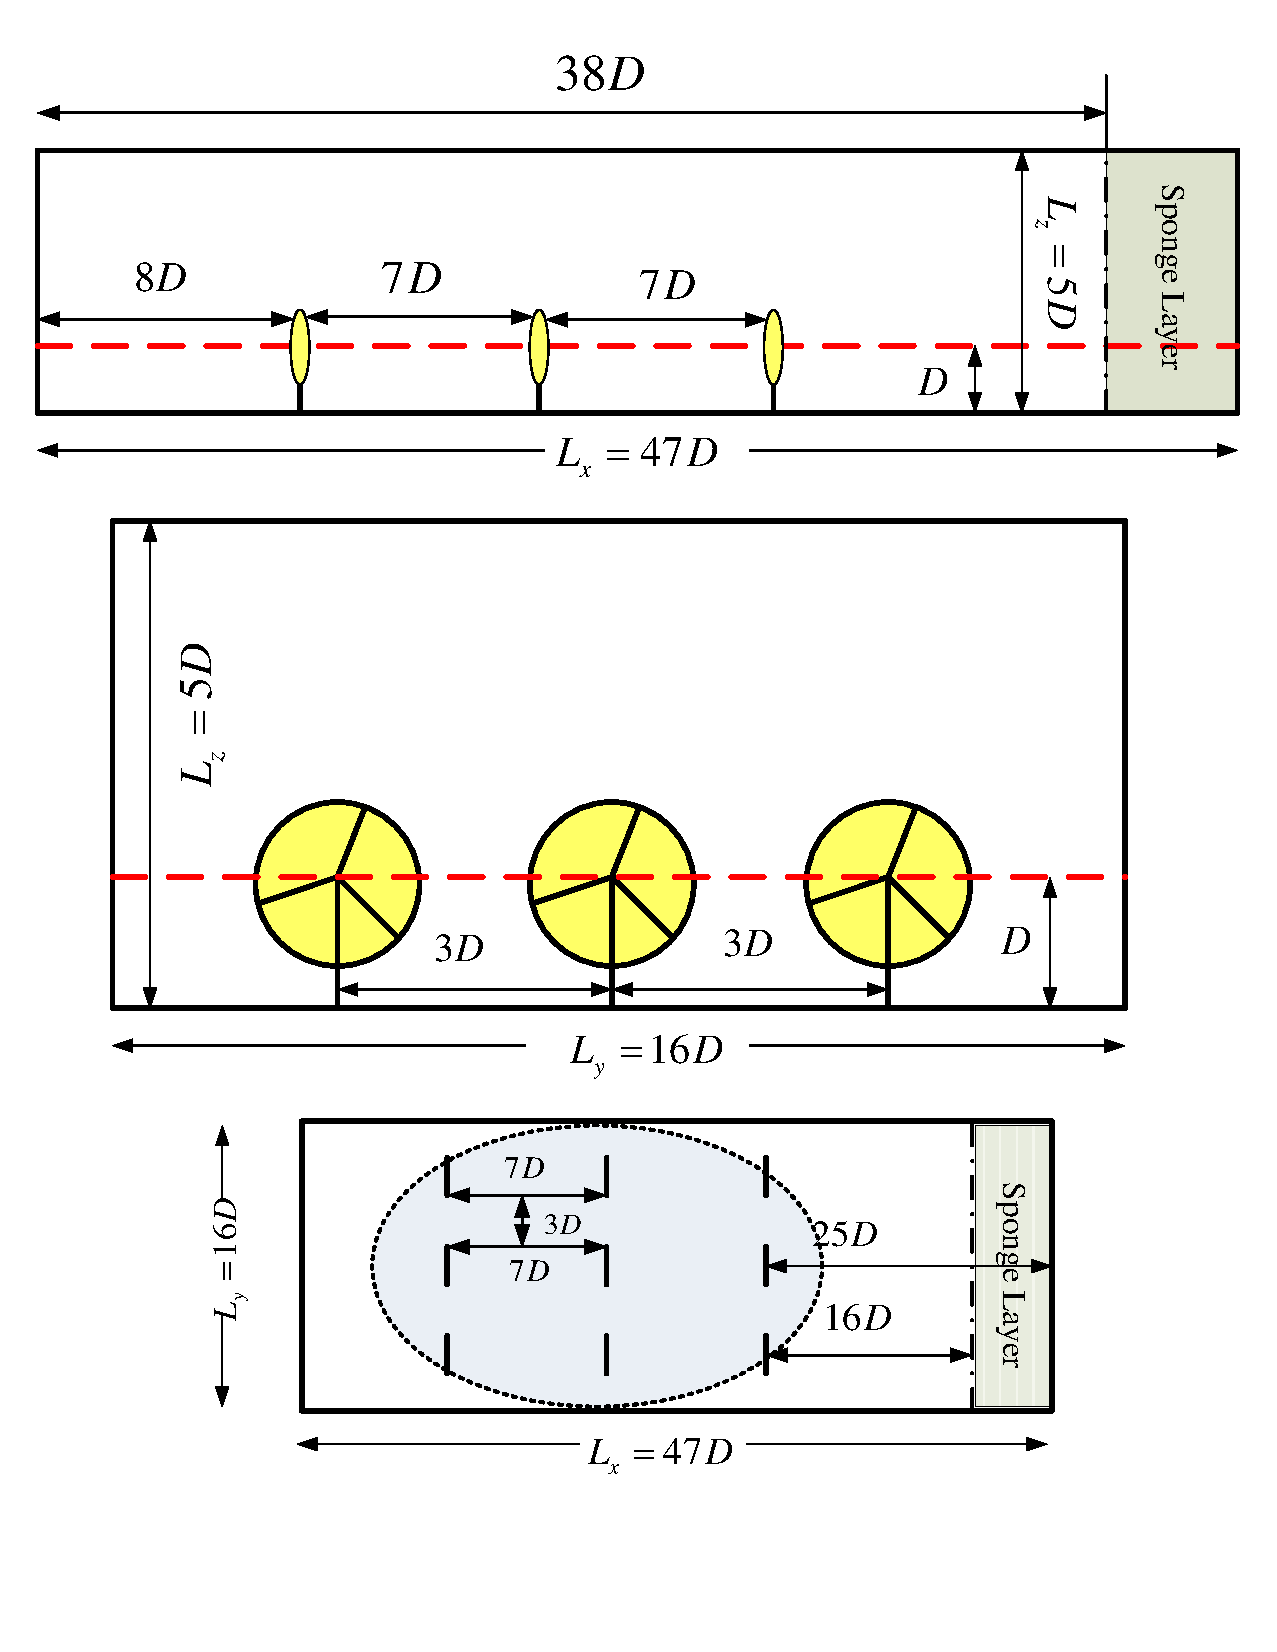
\includegraphics[width=0.55\textwidth]{turbine_array.pdf}\\
 \caption[Computational Domain of Wind turbine array]{Computational domain of wind turbine array AL simulations. top: $x-z$ plane, middle:$y-z$ plane, bottom: $x-y$ plane. The red-dashed line represents the hub-height of the rotors; the dotted ellipse in the bottom figure represents the region of $3\times 3$ wind turbine array}
 \label{f:cord}
\end{figure}
\section{Computational Domain}
The domain size for the actuator line model wind turbine array is $3\pi H\times \pi H\times H$, ($H$ is the ABL boundary layer thickness) with the statistically stationary ABL simulation serving as an initial condition to the actuator line model. Consequently, a seperate ABL simulation at that domain length has been run with a uniform discretization of $40\times 24\times 20$ elements to generate realistic initial conditions for turbine array simulations.  The domain size rescaled in terms of turbine rotor radius (diameter) is given as $94R\times 32R\times 10R \ (47D\times 16D\times 5D) $, where $R = 0.1 H$ is the radius of each turbine-rotor ($D = 2R$ is turbine-rotor diameter). The $9$ turbine rotors have been arranged in a $3\times 3$ matrix arrangement in the computational domain. The design of the  computational domain and the arrangement of different turbines are done in concordance with the experimental set up as in ~\cite{men2,cal3} (See Figure~\ref{f:cord}). 


The first row of 3 rotors are placed at $\pi H/2$ or $8D$ distance from the inflow boundary. The streamwise distance between the turbines is $7D$, while the spanwise distance is $3D$. The hub-height of all the rotors have been set at $D$. These dimensions are designed to conform the experimental set-up as in ~\cite{men2,cal3}. The physical streamwise extent of the domain is $38D$, after which the non-reflective sponge layer initiates with a coarse 2 element stretch to $x = 47D$ coupled with natural outflow boundary condition (See Equation~\ref{nbc1}). Consequently, the wake of last row of 3 sets of rotors has a capacity to convect a physical distance of $16D$ which is more than twice the inter-rotor streamwise spacing. However, for implementing stabilized natural boundary condition~\cite{dong}, it was observed in the previous literature as in ~\cite{erik} that extended domains are still required such that the stabilized boundary conditions do not affect eddies upstream in the flow. The turbulent inflow conditions are implemented as a stationary overlapping mesh methodology~\cite{bem}, where both the simulations are run simultaneously with the inflow condition from ABL simulation being generated by spectrally interpolating the mid-plane of the ABL domain ($yz$ plane at $x = 2\pi\delta$) to the inflow boundary of the computational domain of turbine array (direct memory copies). Since, the spectral interpolation is done in parallel using Message Passing Interface (MPI) it removes the I/O overhead significantly in the computation. \\
\par
The simulations are run with tip-speed ratio $\lambda = 5.00$, (the typical tip-speed ratio for wind turbine is $3-8$) where $\lambda = \Omega R /\overline{V}_x$, with $\Omega$ being the angular velocity of rotor, and $\overline{V}_x$ is the bulk mean stream wise velocity. The pitch angle used in the current simulation $\gamma$ varies linearly between $\ang{0} - \ang{10}$ along the span and the chord-length varies as $C \sim 0.03R - 0.11R$, with various NACA aerofoils being used for the blade corresponding to the study of Troldborg~\cite{troldborg}. The flow velocities at the location where lift and drag forces on the blades are acting are obtained from spectral interpolation technique in Nek5000~\cite{nek5000-web-page}. The drag forces experienced by the cylindrical nacelle and the turbine tower has been modelled by using a simple model using $F_{drag} = \frac{1}{2}C_D \rho U_{bulk}^2 A$, with $C_D \sim 0.9 \ , 1.5$ and $A$ the cross-sectional area for the nacelle and tower respectively in the current simulations. The subgrid scale model remains the same as in ABL simulations (See Chapter~\ref{Chapter3}). However, in the AL model~\cite{troldborg,peet2}, it was observed that approximately 30 points were required in the blade-span ($y-z$ direction) to resolve the wakes behind turbine arrays, demanding a local refinement of the grid of computational domain near the turbines in the $y-z$ plane~\cite{troldborg,churchfield,peet2,tan}. The refinement was performed by considering a base grid of ABL simulation (used in initial condition of turbine array) with domain size $3\pi H \times \pi H \times H$ using $40\times 24\times 20$ elements and shown on Table~\ref{table:grid2}.


\begin{table}[ht] 
\centering % used for centering table 
\begin{tabular}{c c c c} % centered columns (4 columns) 
\hline\hline    %inserts double horizontal lines 
Case & Geometry & $N^{e}_x\times N^{e}_y\times N^{e}_z$  & Grid points   \\ [0.5 ex] % inserts table 
%heading 
\hline  % inserts single horizontal line 
Sponge Layer & $3\pi H \times \pi H \times H$ & $42\times 32\times 24$ & $1.122\times 10^7$ \\ % inserting body of the table 
Stabilized NBC (Dong et. al) & $3\pi H \times \pi H \times H$ & $48\times 32\times 24$ & $1.281\times 10^7$  \\ [1ex] % [1ex] adds vertical space 
\hline\hline \\ [1 ex]
\end{tabular} 
\caption[Wind turbine array: Computational Domain]{Numerical setup for wind turbine array computational domain for two different outflow boundaries. 8 GLL nodes has been used per cartesian direction } % title of Table 
\label{table:grid2} % is used to refer this table in the text 
\end{table} 
Simultaneous refinement in the streamwise direction is also of crucial importance, as far as resolving the wakes of the turbine arrays is concerned. It was observed, that without proper resolution in the streamwise direction, spurious modes develop upstream of the turbine and pollute the flow (See ~\cite{tan}). Additionally, nodal interpolation filter of spectral accuracy~\cite{fischer_filter} has been applied on the two highest modes to eliminate the spurious modes. The non-dimensional timestep has been chosen to be $tD/U_{bulk} \ \sim 3.5\times 10^{-4}$ not only to ensure numerical stability, but also in a way that the rotational motion of the actuator line element is restricted by not covering more than a near turbine element in a timestep. (resolving temporal scales of wakes).  The aerodynamic roughness is taken to be $z_0 = 10^{-4}H$ (constant similar to ~\cite{porte2a,porte1fun}) for both neutral ABL simulations (Chapter~\ref{Chapter3}) and actuator line simulations involving turbine arrays (Chapter~\ref{Chapter4}). The first grid node away from the wall for wind turbine array simulation is such that $\Delta z/z_0$ is identical to the ABL simulation.

\section{Results: Mean and Second order statistics}
\begin{figure}
\centering
        \begin{subfigure}[t]{0.5\textwidth}
                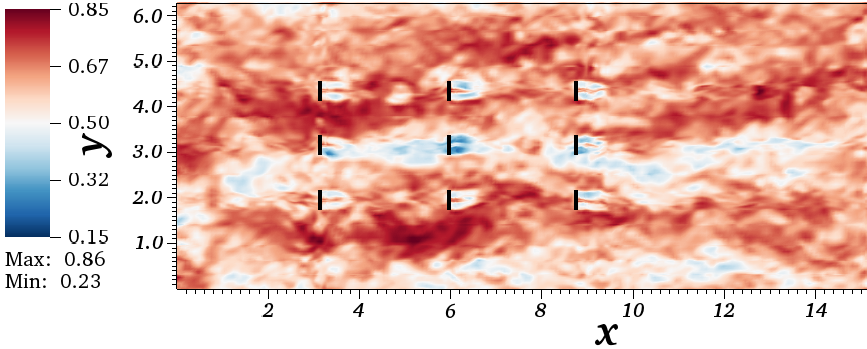
\includegraphics[width=\linewidth]{movie_xy_cropped/movie_xy_2.png}
                \caption{}
                \label{fig:snap1}
        \end{subfigure}%
        \centering
        \begin{subfigure}[t]{0.5\textwidth}
                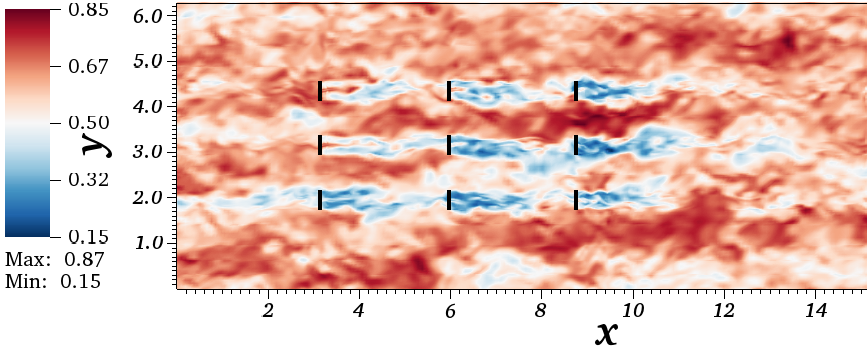
\includegraphics[width=\linewidth]{movie_xy_cropped/movie_xy_12.png}
                \caption{}
                \label{fig:snap2}
        \end{subfigure}
       \centering
        \begin{subfigure}[t]{0.5\textwidth}
                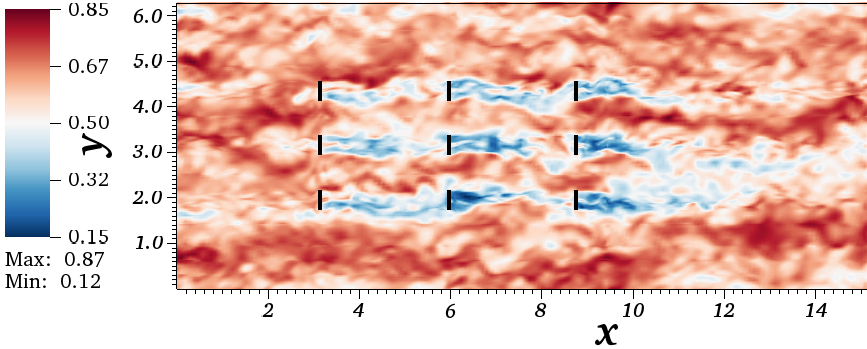
\includegraphics[width=\linewidth]{movie_xy_cropped/movie_xy_19.png}
                \caption{}
                \label{fig:snap3}
        \end{subfigure}%
        \centering
        \begin{subfigure}[t]{0.5\textwidth}
                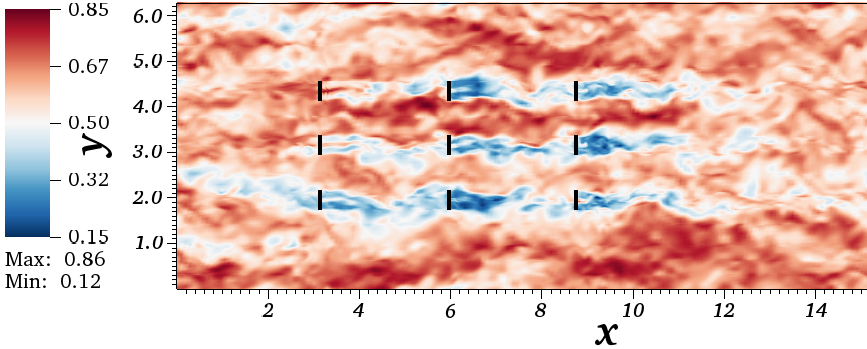
\includegraphics[width=\linewidth]{movie_xy_cropped/movie_xy_26.png}
                \caption{}
                \label{fig:snap4}
        \end{subfigure}
     \centering
        \begin{subfigure}[t]{0.5\textwidth}
                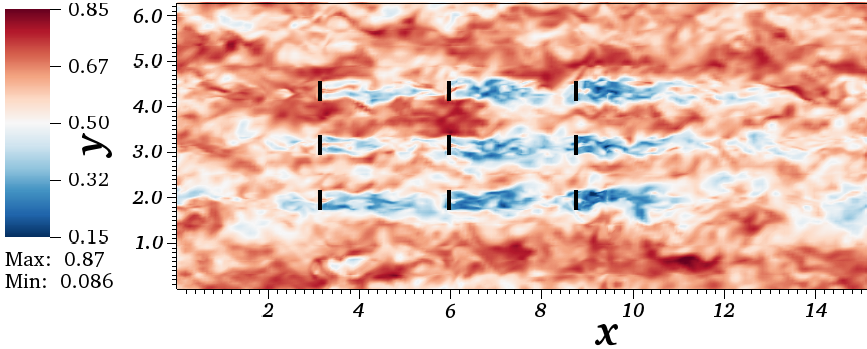
\includegraphics[width=\linewidth]{movie_xy_cropped/movie_xy_33.png}
                \caption{}
                \label{fig:snap5}
        \end{subfigure}%
        \centering
        \begin{subfigure}[t]{0.5\textwidth}
                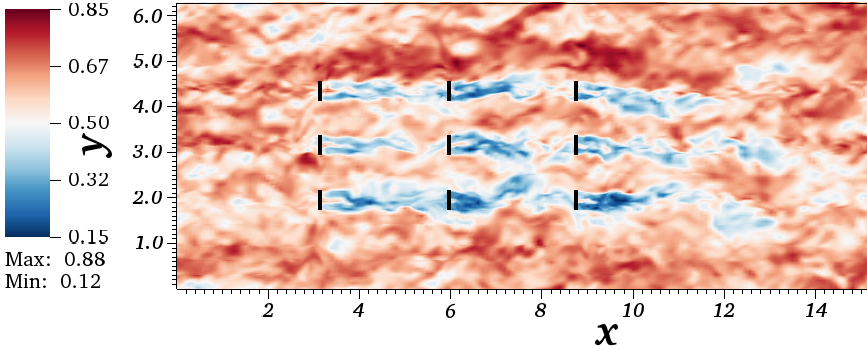
\includegraphics[width=\linewidth]{movie_xy_cropped/movie_xy_38.png}
                \caption{}
                \label{fig:snap6}
        \end{subfigure}
        \caption[Temporal Snapshots in $xy$ plane]{Snapshots of turbulent flow past the wind turbine array in streamwise-spanwise ($xy$) plane at different time levels.}\label{fig:snap_xy}
\end{figure}


\begin{figure}
\centering
        \begin{subfigure}[t]{0.85\textwidth}
                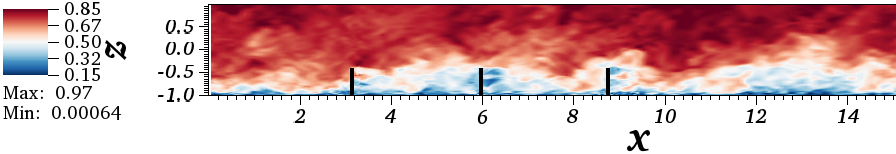
\includegraphics[width=\linewidth]{movie_xz_cropped/movie_xz_2.png}
                \caption{}
                \label{fig:snap1}
        \end{subfigure}
        \centering
        \begin{subfigure}[t]{0.85\textwidth}
                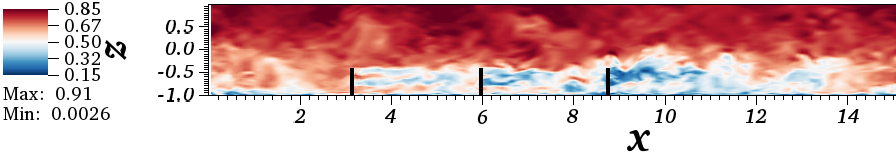
\includegraphics[width=\linewidth]{movie_xz_cropped/movie_xz_12.png}
                \caption{}
                \label{fig:snap2}
        \end{subfigure}
       \centering
        \begin{subfigure}[t]{0.85\textwidth}
                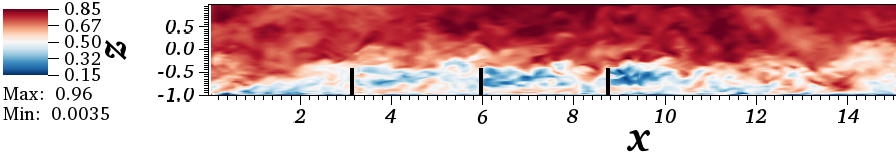
\includegraphics[width=\linewidth]{movie_xz_cropped/movie_xz_19.png}
                \caption{}
                \label{fig:snap3}
        \end{subfigure}
        \centering
        \begin{subfigure}[t]{0.85\textwidth}
                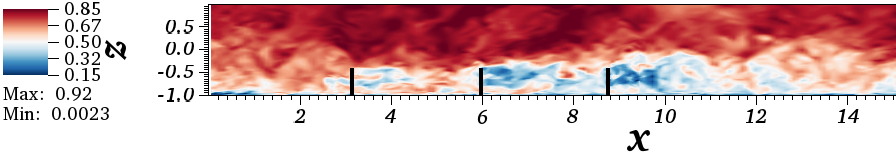
\includegraphics[width=\linewidth]{movie_xz_cropped/movie_xz_26.png}
                \caption{}
                \label{fig:snap4}
        \end{subfigure}
     \centering
        \begin{subfigure}[t]{0.85\textwidth}
                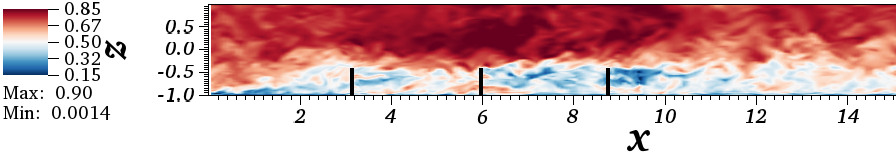
\includegraphics[width=\linewidth]{movie_xz_cropped/movie_xz_33.png}
                \caption{}
                \label{fig:snap5}
        \end{subfigure}
        \centering
        \begin{subfigure}[t]{0.85\textwidth}
                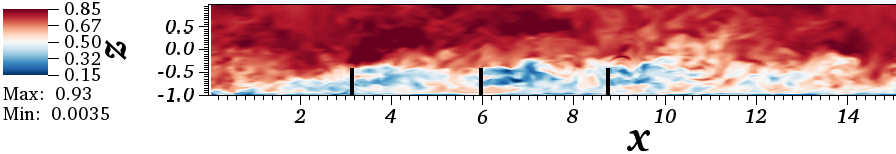
\includegraphics[width=\linewidth]{movie_xz_cropped/movie_xz_38.png}
                \caption{}
                \label{fig:snap6}
        \end{subfigure}
        \caption[Temporal Snapshots in $xy$ plane]{Snapshots of turbulent flow past the wind turbine array in streamwise-wall normal ($xz$) plane at different time levels.}\label{fig:snap_xz}
\end{figure}

\begin{figure}
\centering
        \begin{subfigure}[t]{0.35\textwidth}
                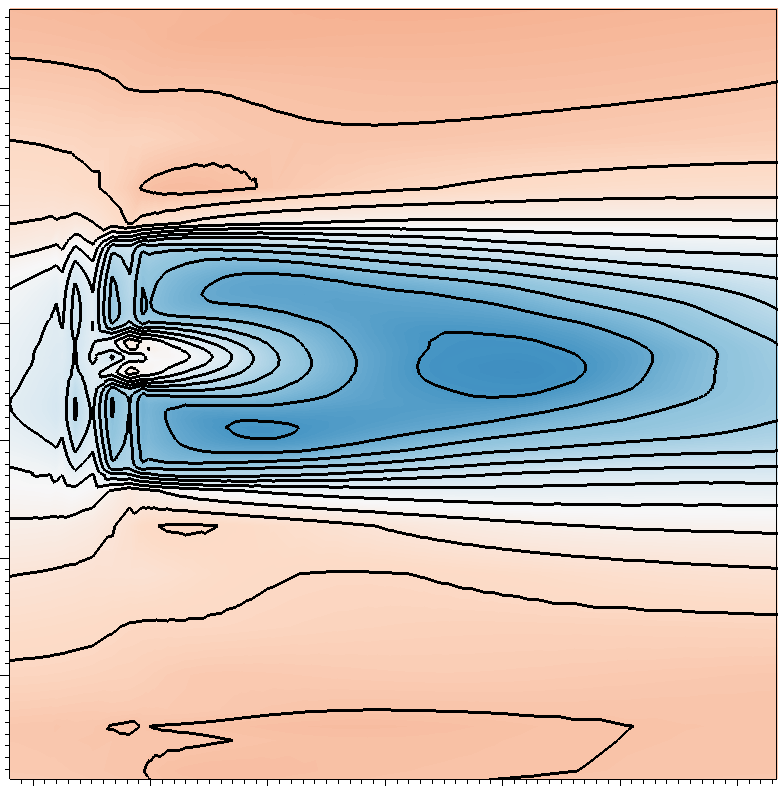
\includegraphics[width=\linewidth]{Figure/avg_lines.png}
                \caption{}
                \label{fig:ss1}
        \end{subfigure}%
        \centering
        \begin{subfigure}[t]{0.55\textwidth}
                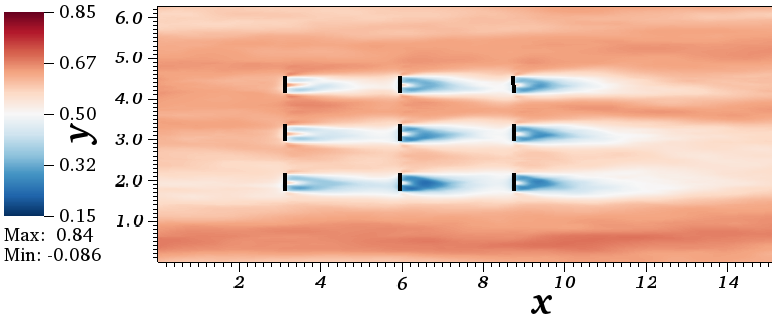
\includegraphics[width=\linewidth]{Figure/avg_2.png}
                \caption{}
                \label{fig:ss2}
        \end{subfigure}
        \centering
        \begin{subfigure}[t]{0.75\textwidth}
                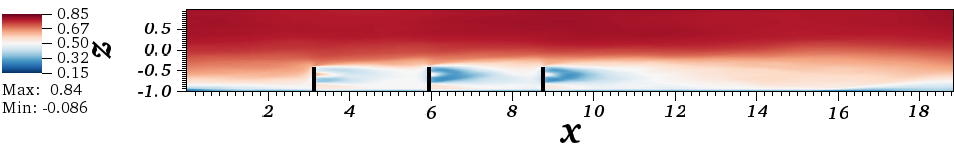
\includegraphics[width=\linewidth]{Figure/avg_3.png}
                \caption{}
                \label{fig:ss2b}
        \end{subfigure}
       \centering
        \begin{subfigure}[t]{0.75\textwidth}
                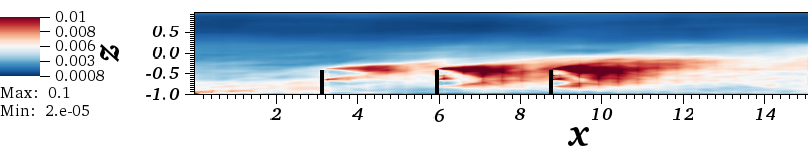
\includegraphics[width=\linewidth]{Figure/tke.png}
                \caption{}
                \label{fig:ss3}
        \end{subfigure}
       \centering
        \begin{subfigure}[t]{0.75\textwidth}
                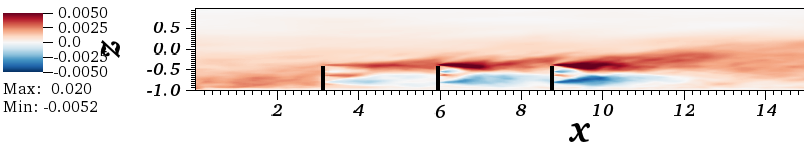
\includegraphics[width=\linewidth]{Figure/uv_shear.png}
                \caption{}
                \label{fig:ss4}
        \end{subfigure}%
        \caption[Temporally Averaged Statistics Contours]{Temporally averaged statistics contour. (A) Contour lines of a wake depicting its symmetric nature about core and wake growth in $xy$ plane. (B) Contour plot of streamwise mean velocity in $xy$ plane. (C) Contour plot of streamwise mean velocity in $xz$ plane. (D) Contour plot of turbulent kinetic energy in $xz$ plane. (E) Contour plot of kinematic shear stress in $xz$ plane.} \label{fig:stress_contours}
\end{figure}

%\begin{figure}
%\centering
%        \begin{subfigure}[t]{0.5\textwidth}
%                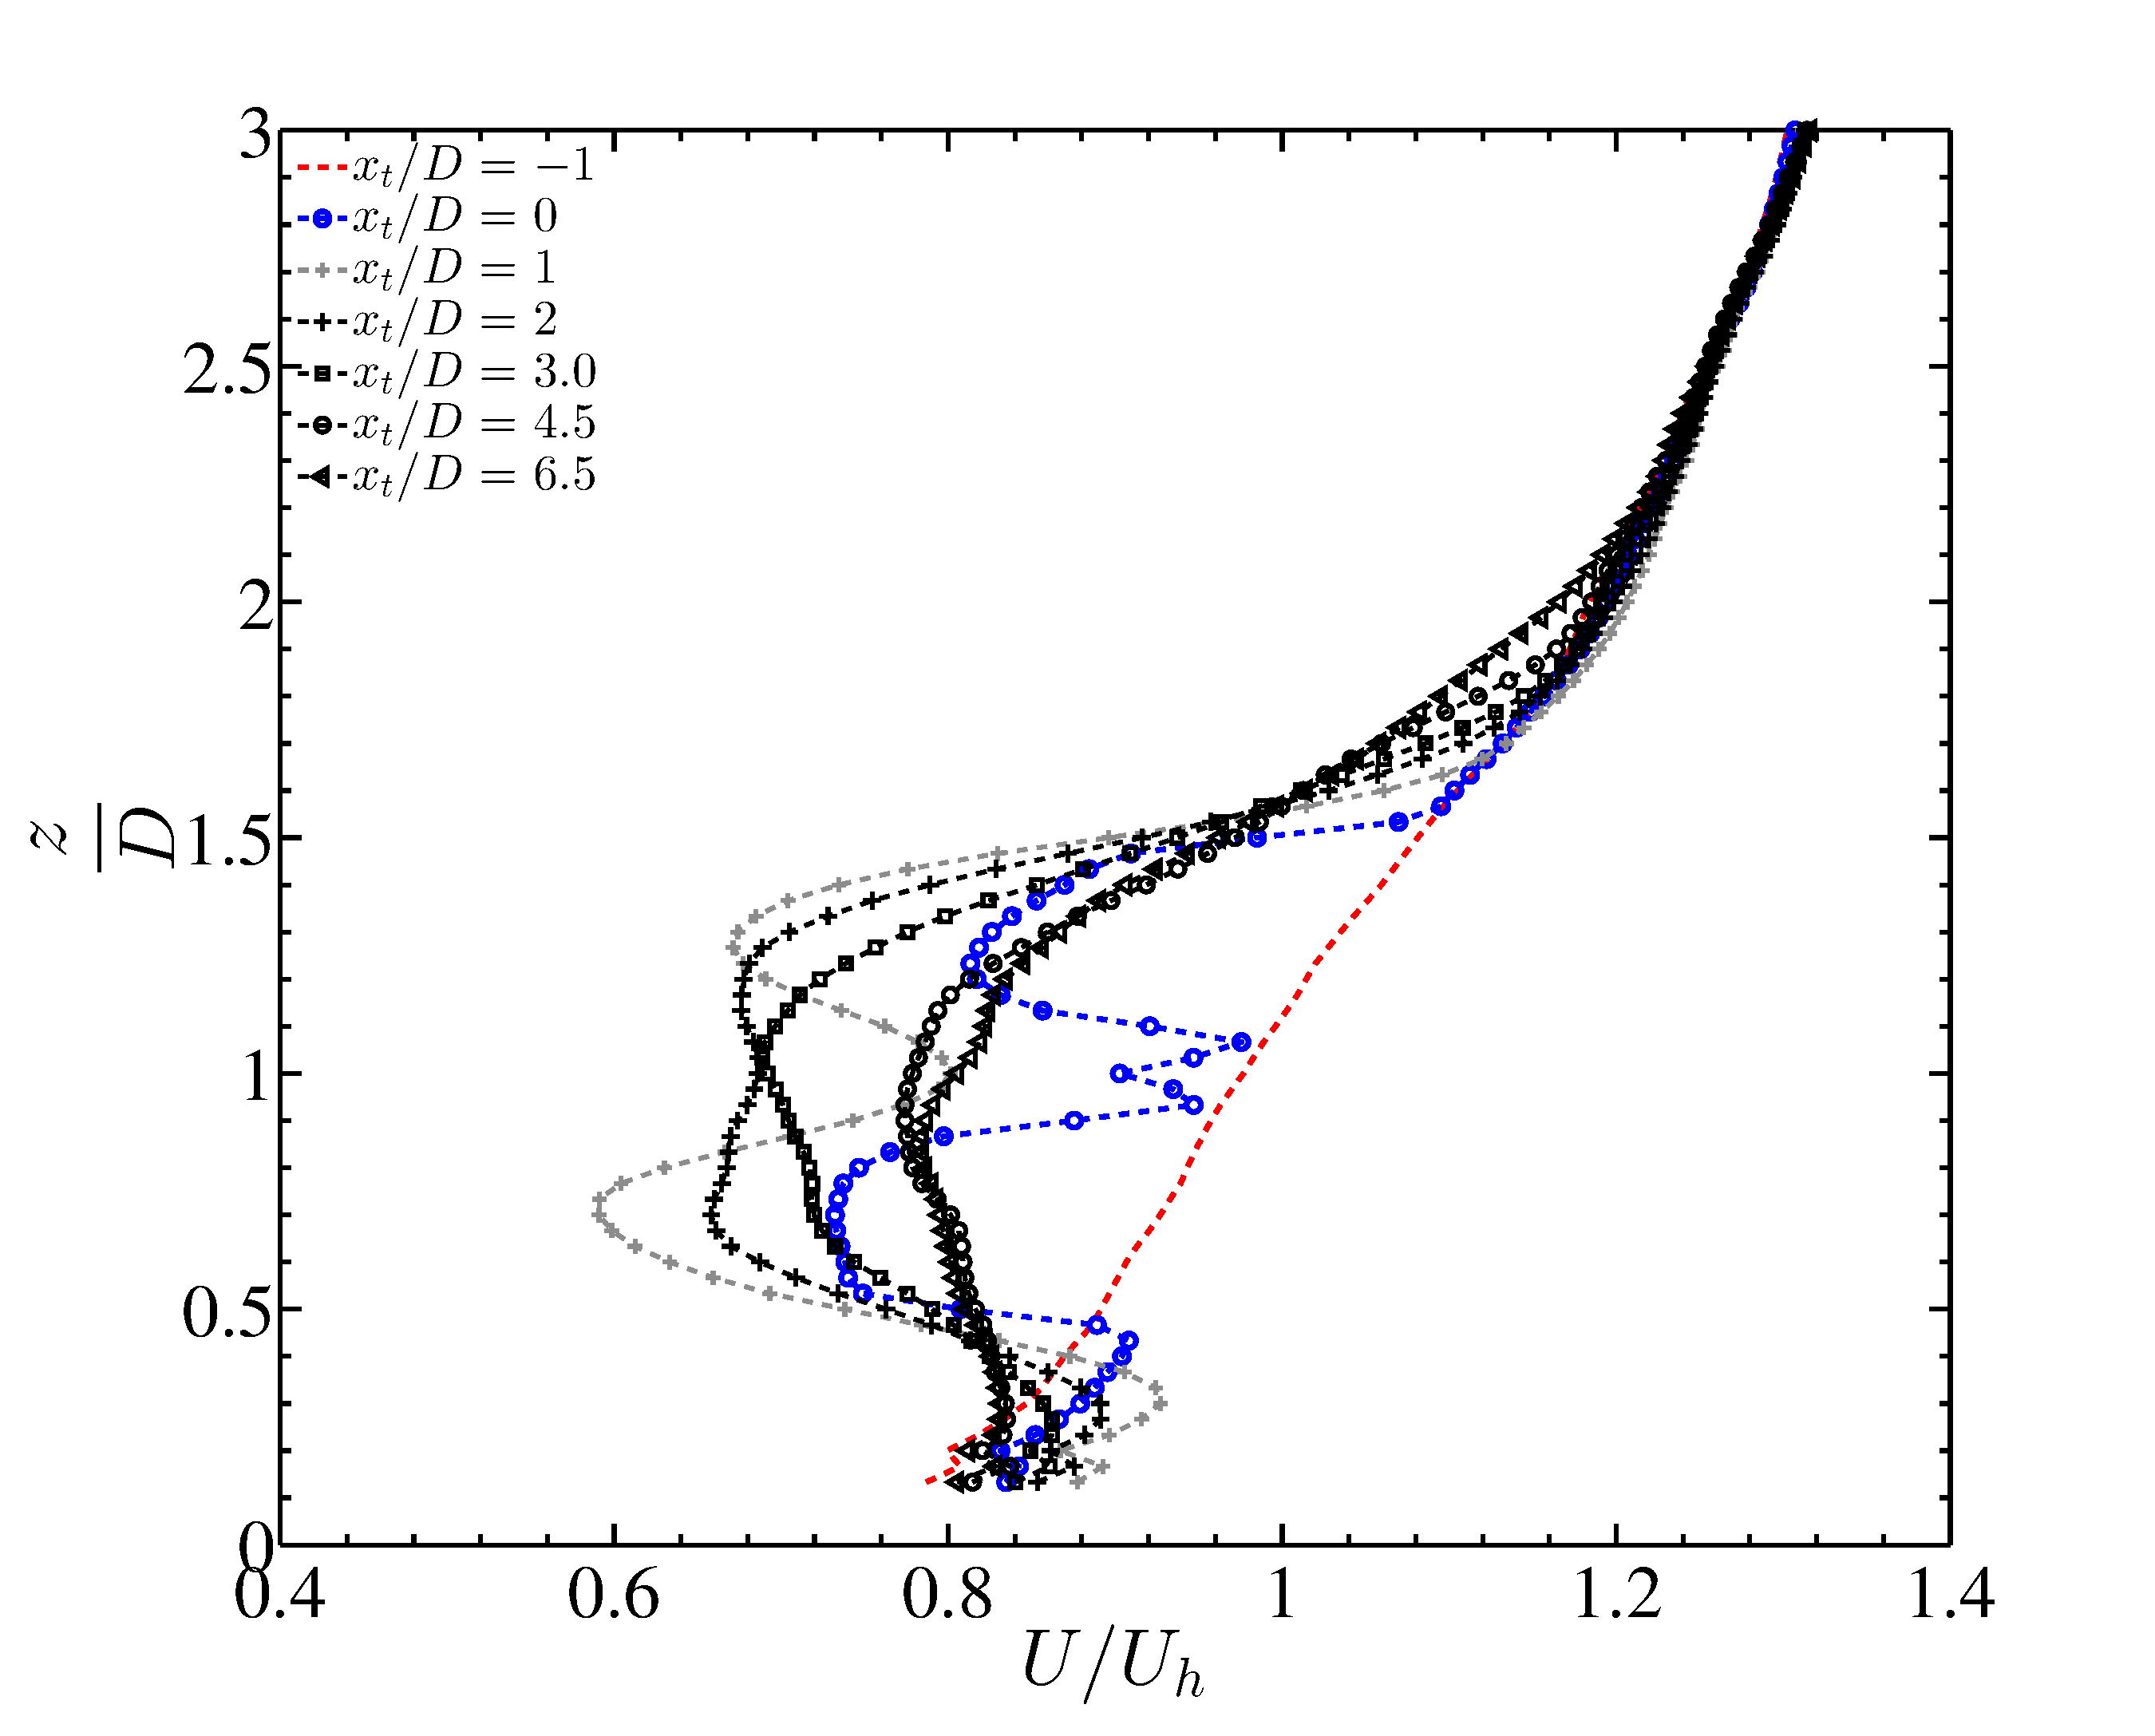
\includegraphics[width=\linewidth]{stats/velocity_profiles_notaveraged.pdf}
%                \caption{}
%                \label{fig:mean1}
%        \end{subfigure}%
%        \centering
%        \begin{subfigure}[t]{0.5\textwidth}
%                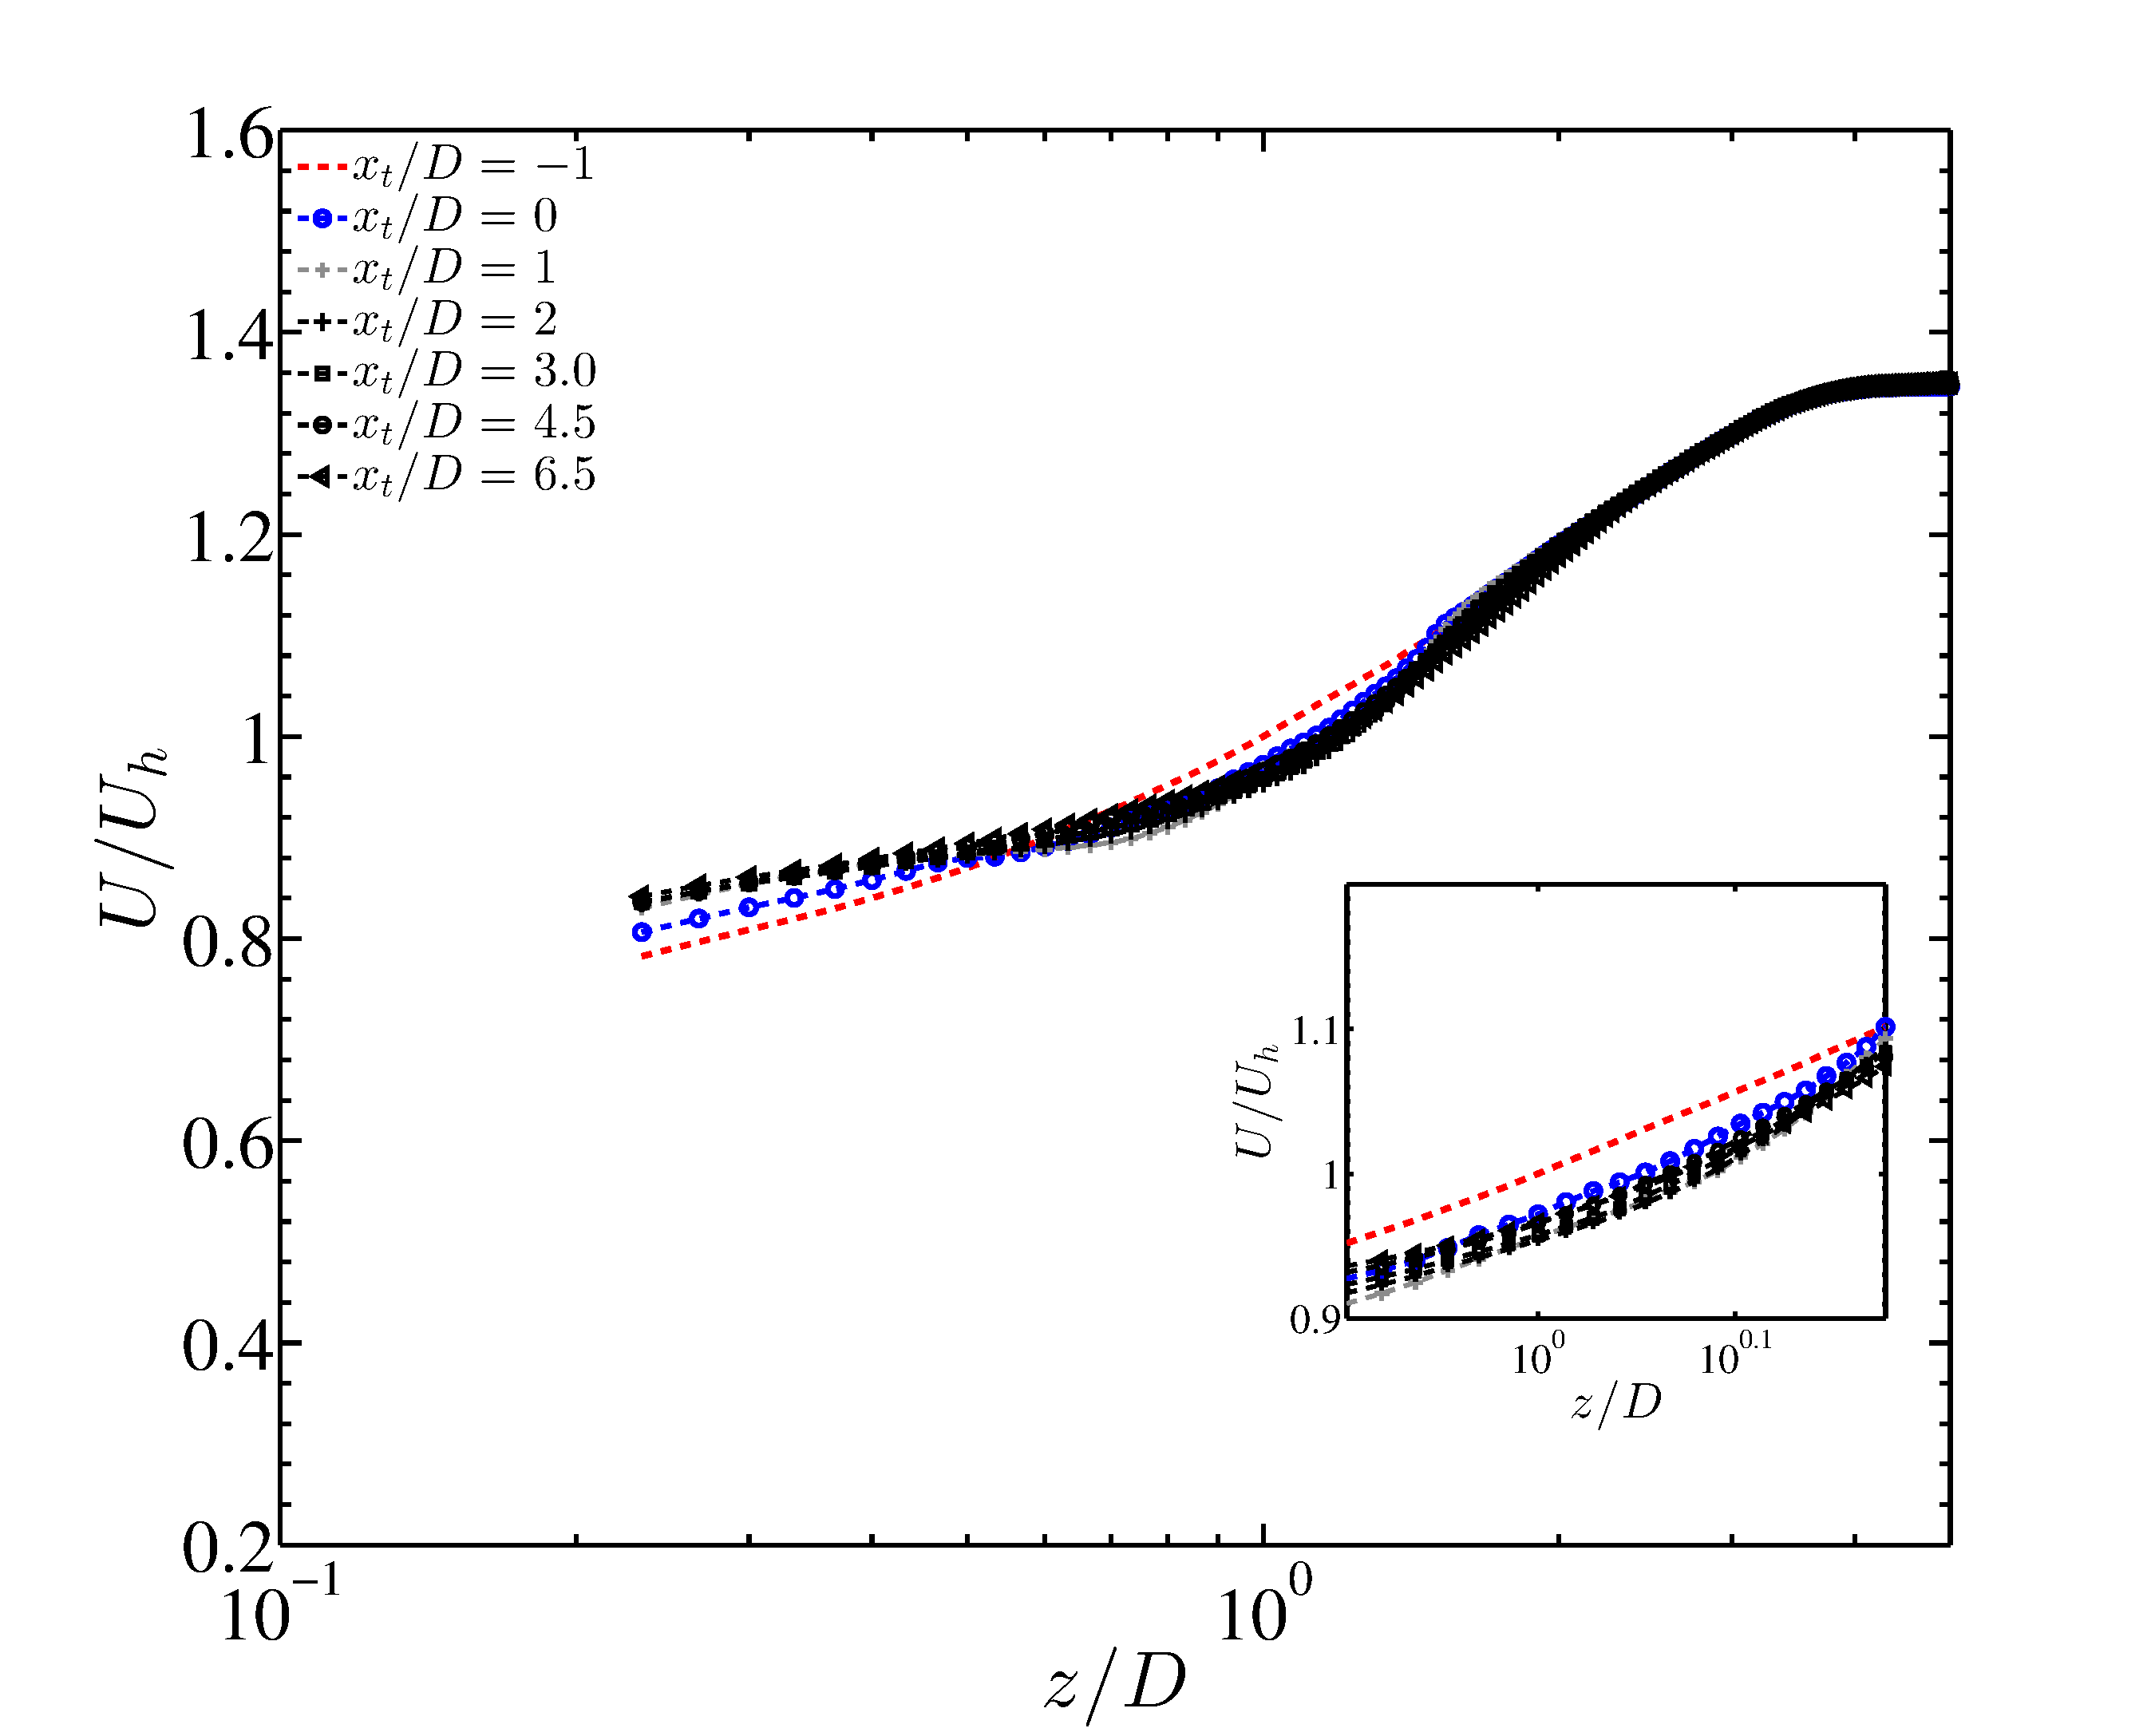
\includegraphics[width=\linewidth]{stats/velprof_3avg_log2.pdf}
%                \caption{}
%                \label{fig:mean2}
%        \end{subfigure}
%        \caption{} \label{fig:mean_stats1}
%\end{figure}
    
%------------------ single figures ----------------------%
\begin{figure}
\centering
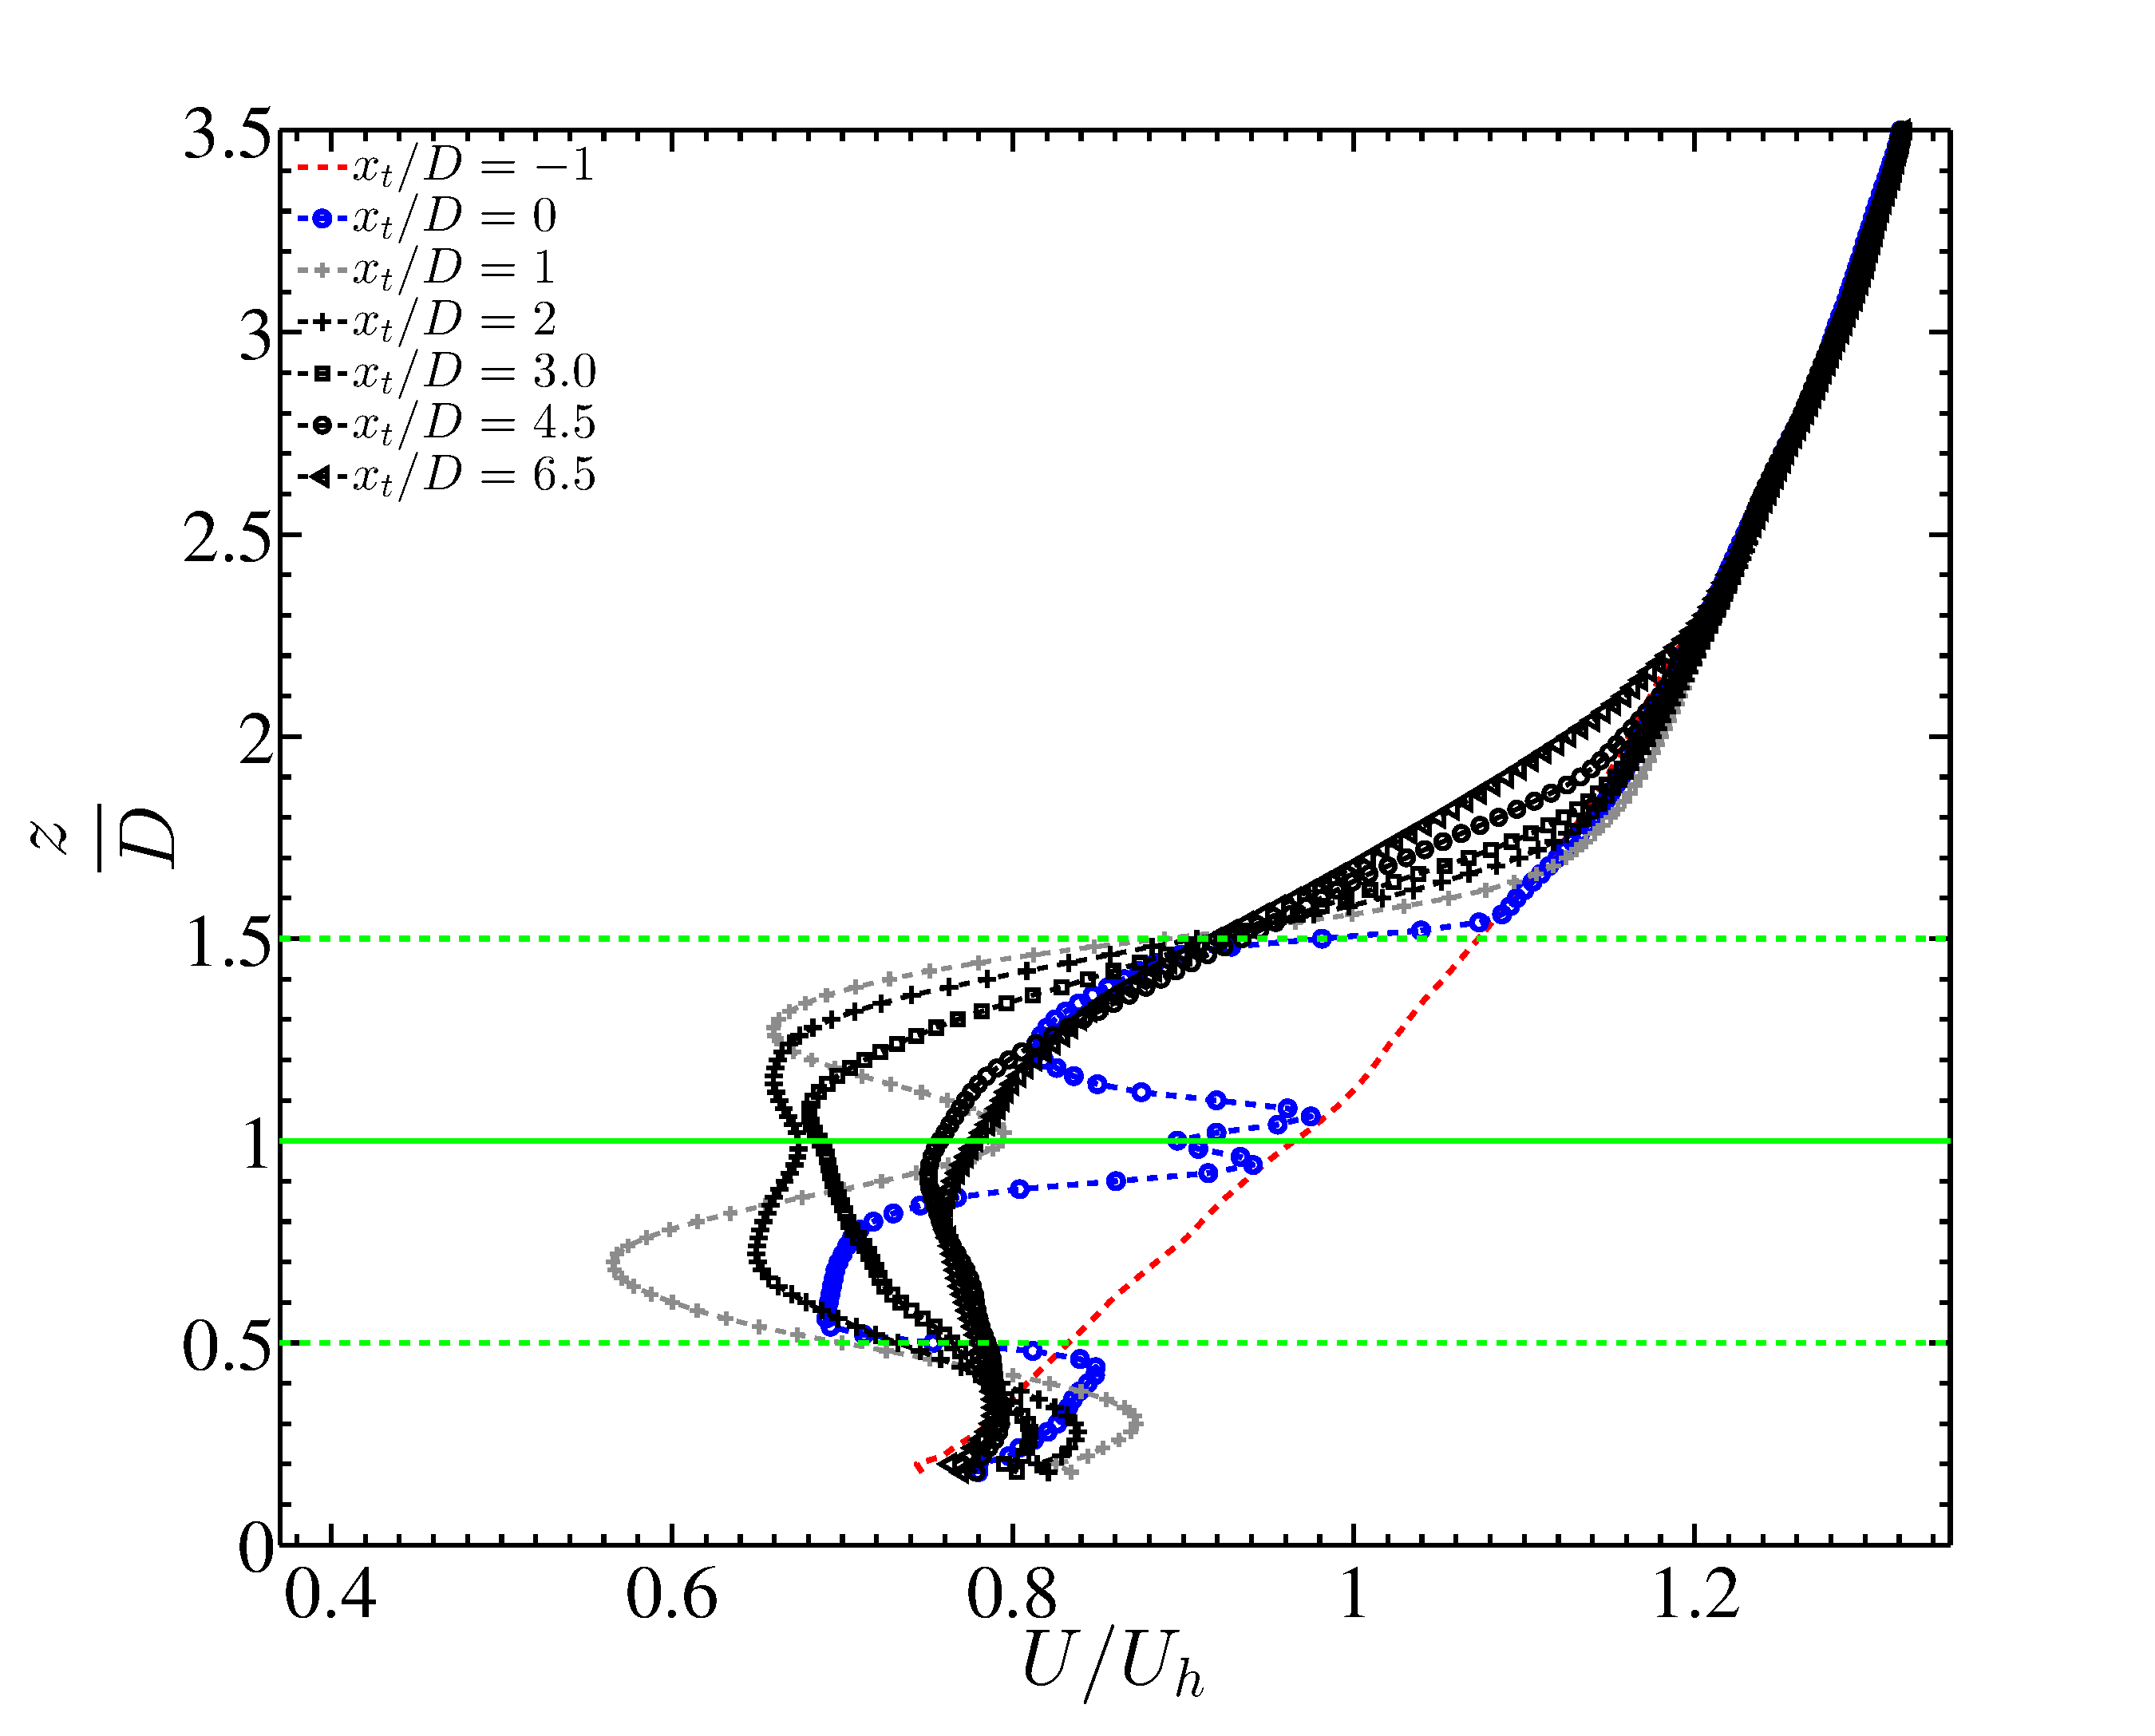
\includegraphics[width = 0.8\linewidth]{stats/velprof_3points_avg.pdf}
\caption[Mean streamwise velocity at $x$ stations 1]{Temporally averaged mean streamwise velocity profile at different streamwise $x$ stations. Profile averaged over the  3 spanwise points (center of turbine rotor).}\label{fig:meanstat1}
\end{figure}
\begin{figure}
\centering
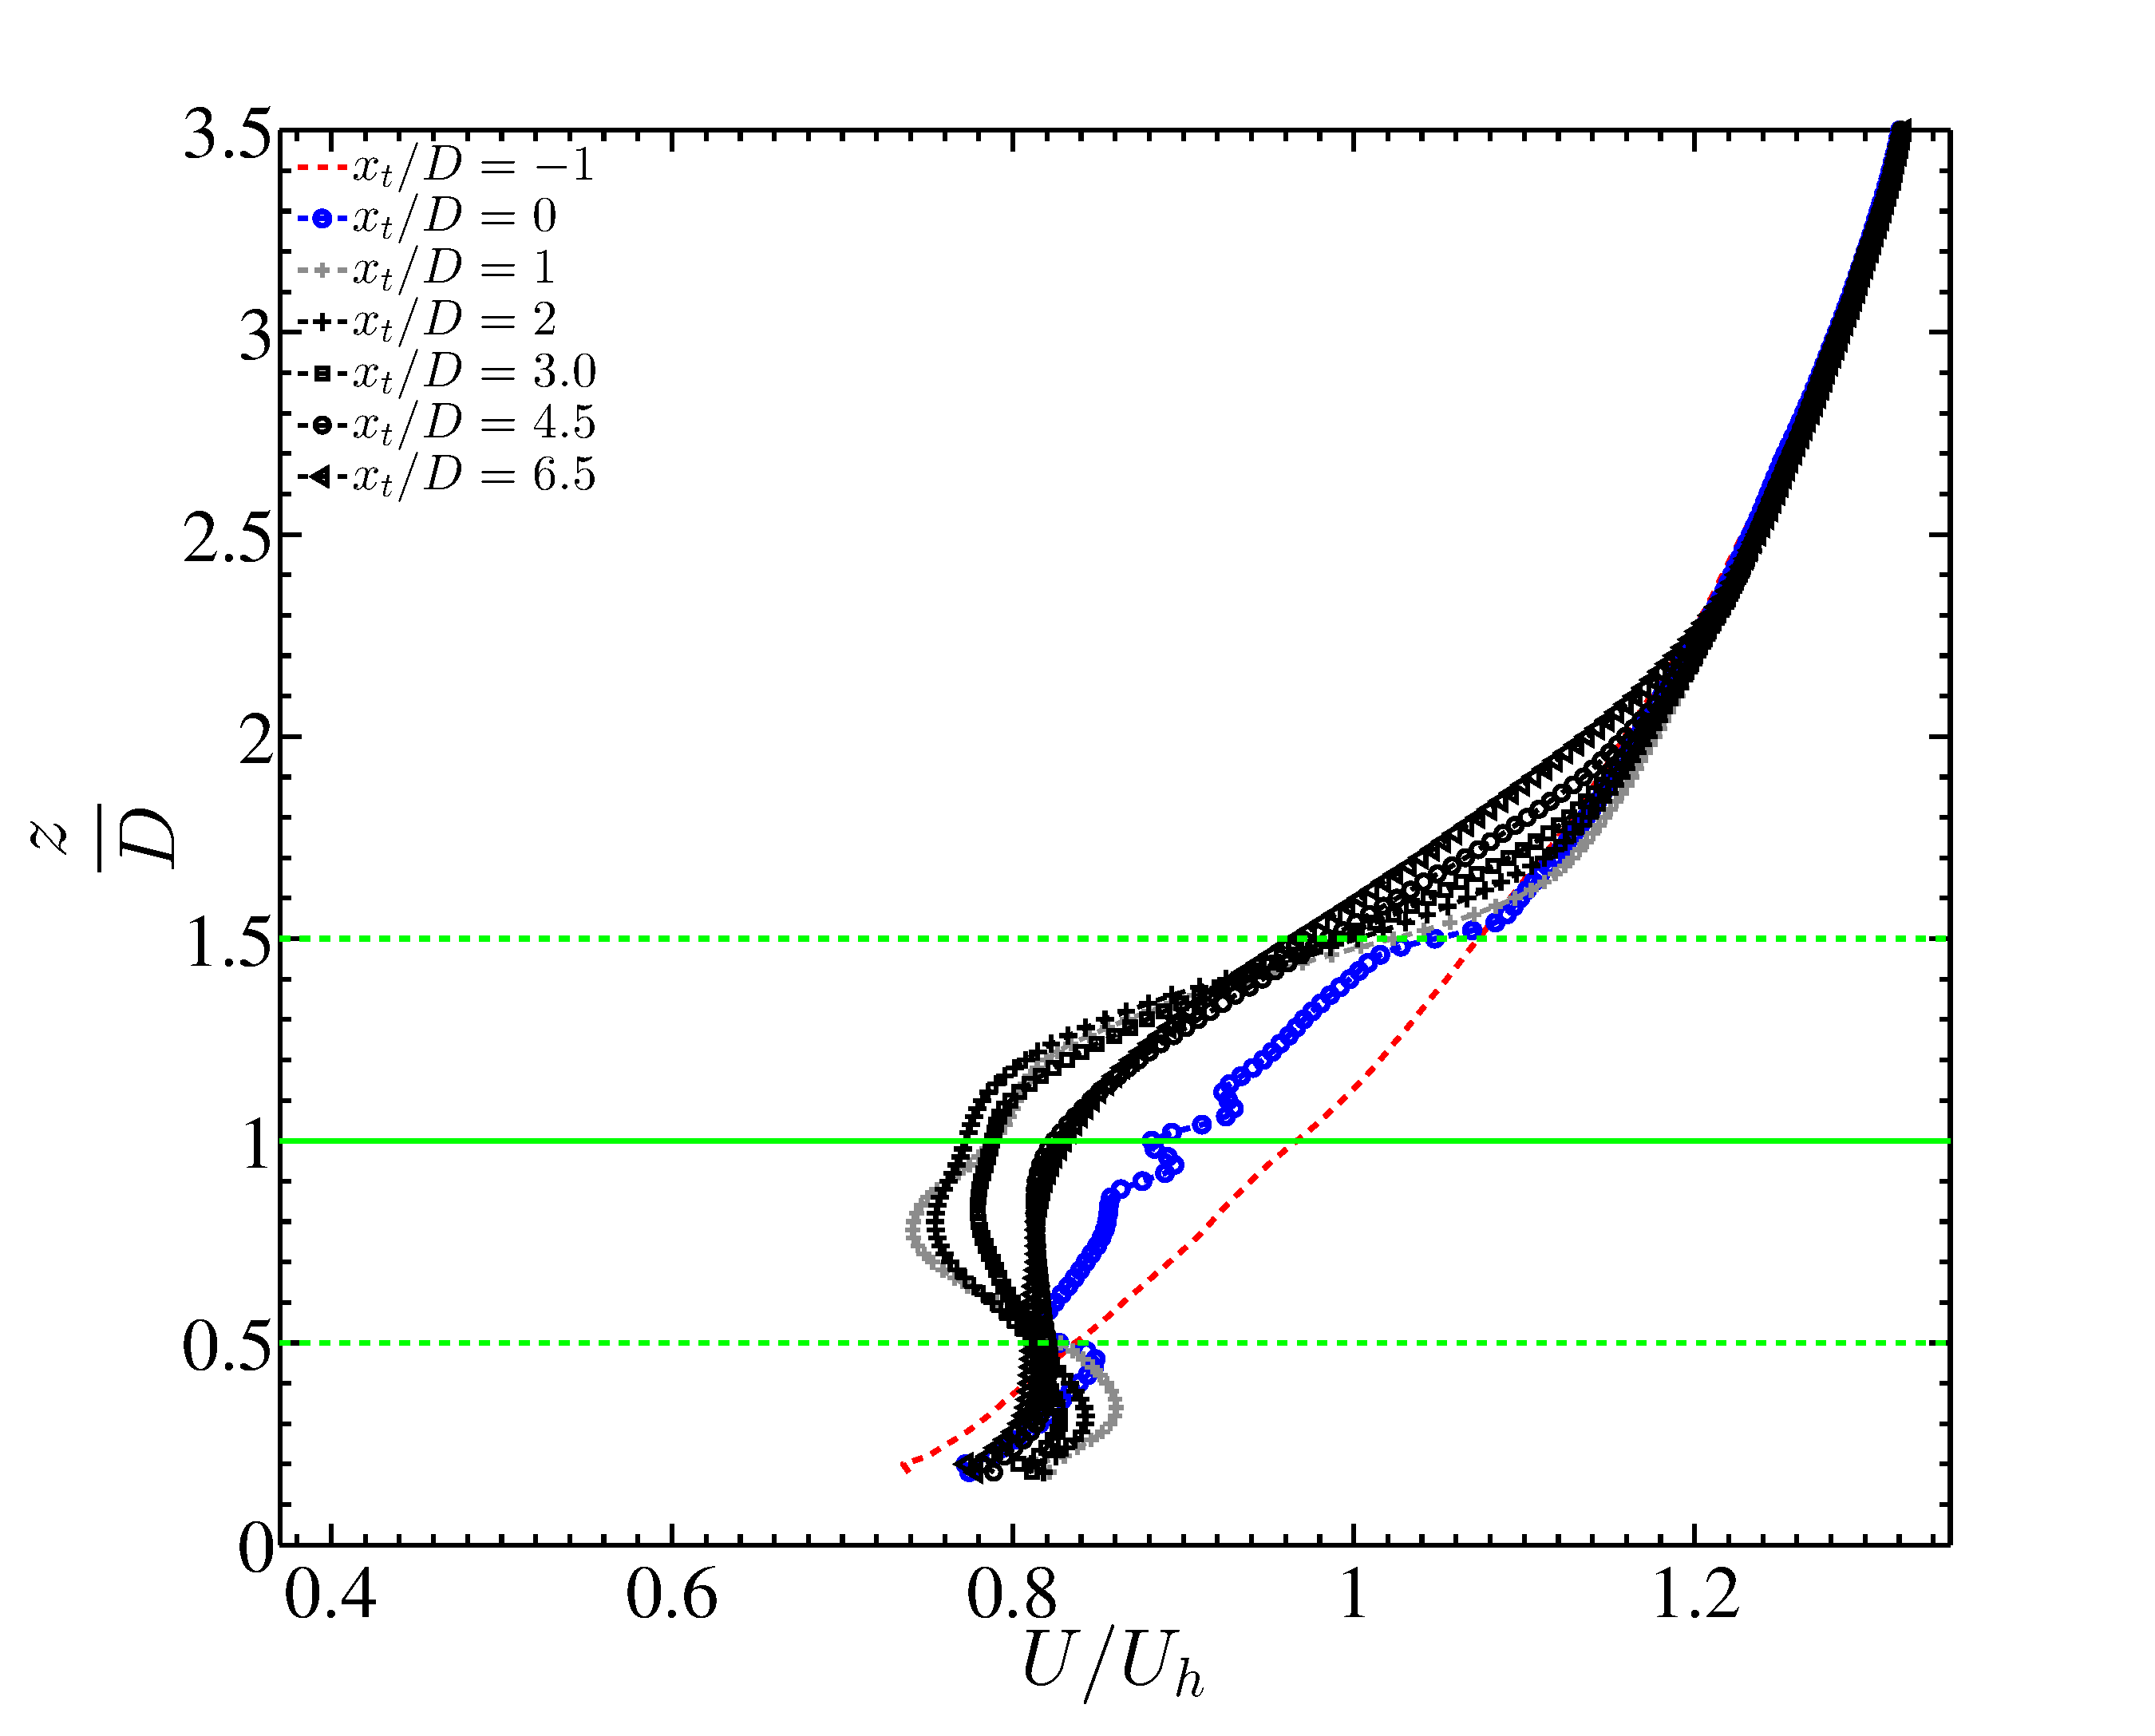
\includegraphics[width = 0.8\linewidth]{stats/velprof_9points_avg.pdf}
\caption[Mean streamwise velocity at $x$ stations 2]{Temporally averaged mean streamwise velocity profile at different streamwise $x$ stations. Profile averaged over the  9 spanwise points over 3 wind turbine rotor extents.}\label{fig:meanstat2}
\end{figure}
\begin{figure}
\centering
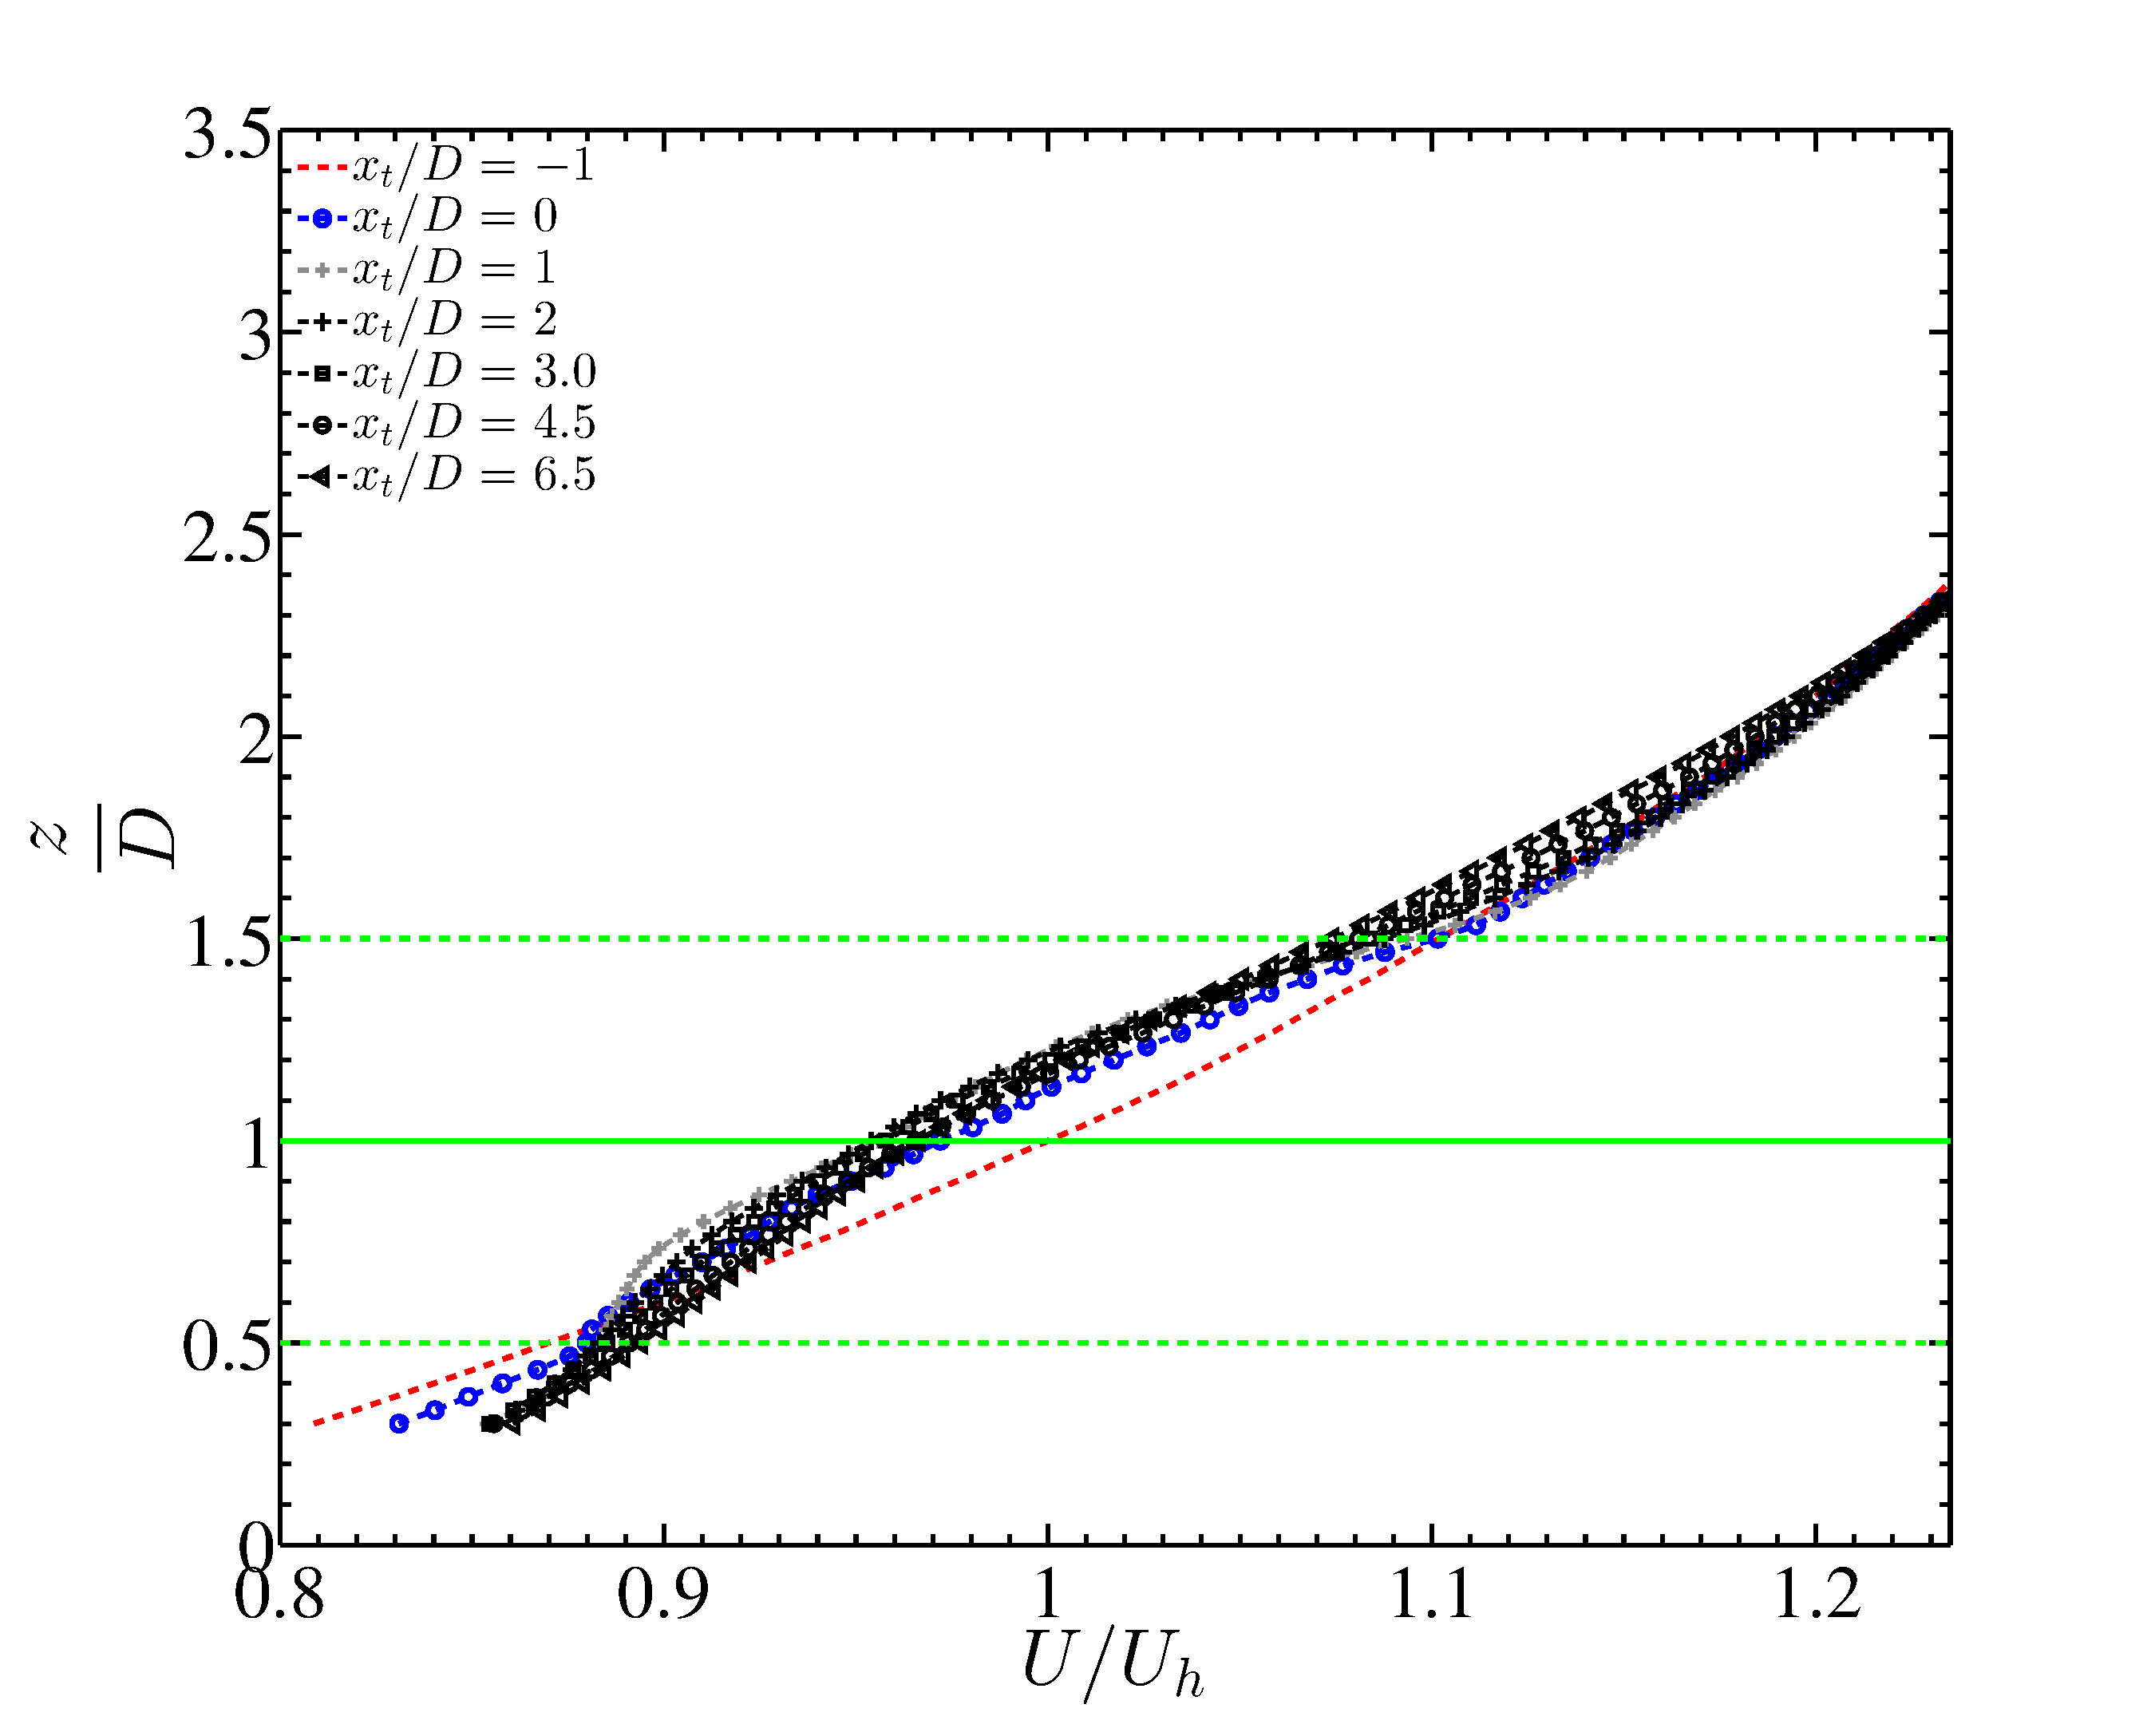
\includegraphics[width = 0.8\linewidth]{stats/velprof_Npoints_avg.pdf}
\caption[Mean streamwise velocity at $x$ stations 3]{Temporally averaged mean streamwise velocity profile at different streamwise $x$ stations. Profile averaged over the whole spanwise domain. }\label{meanstat3}
\end{figure}


%----------------- similarity tests --------------------%
\begin{figure}
\centering
        \begin{subfigure}[t]{0.5\textwidth}
                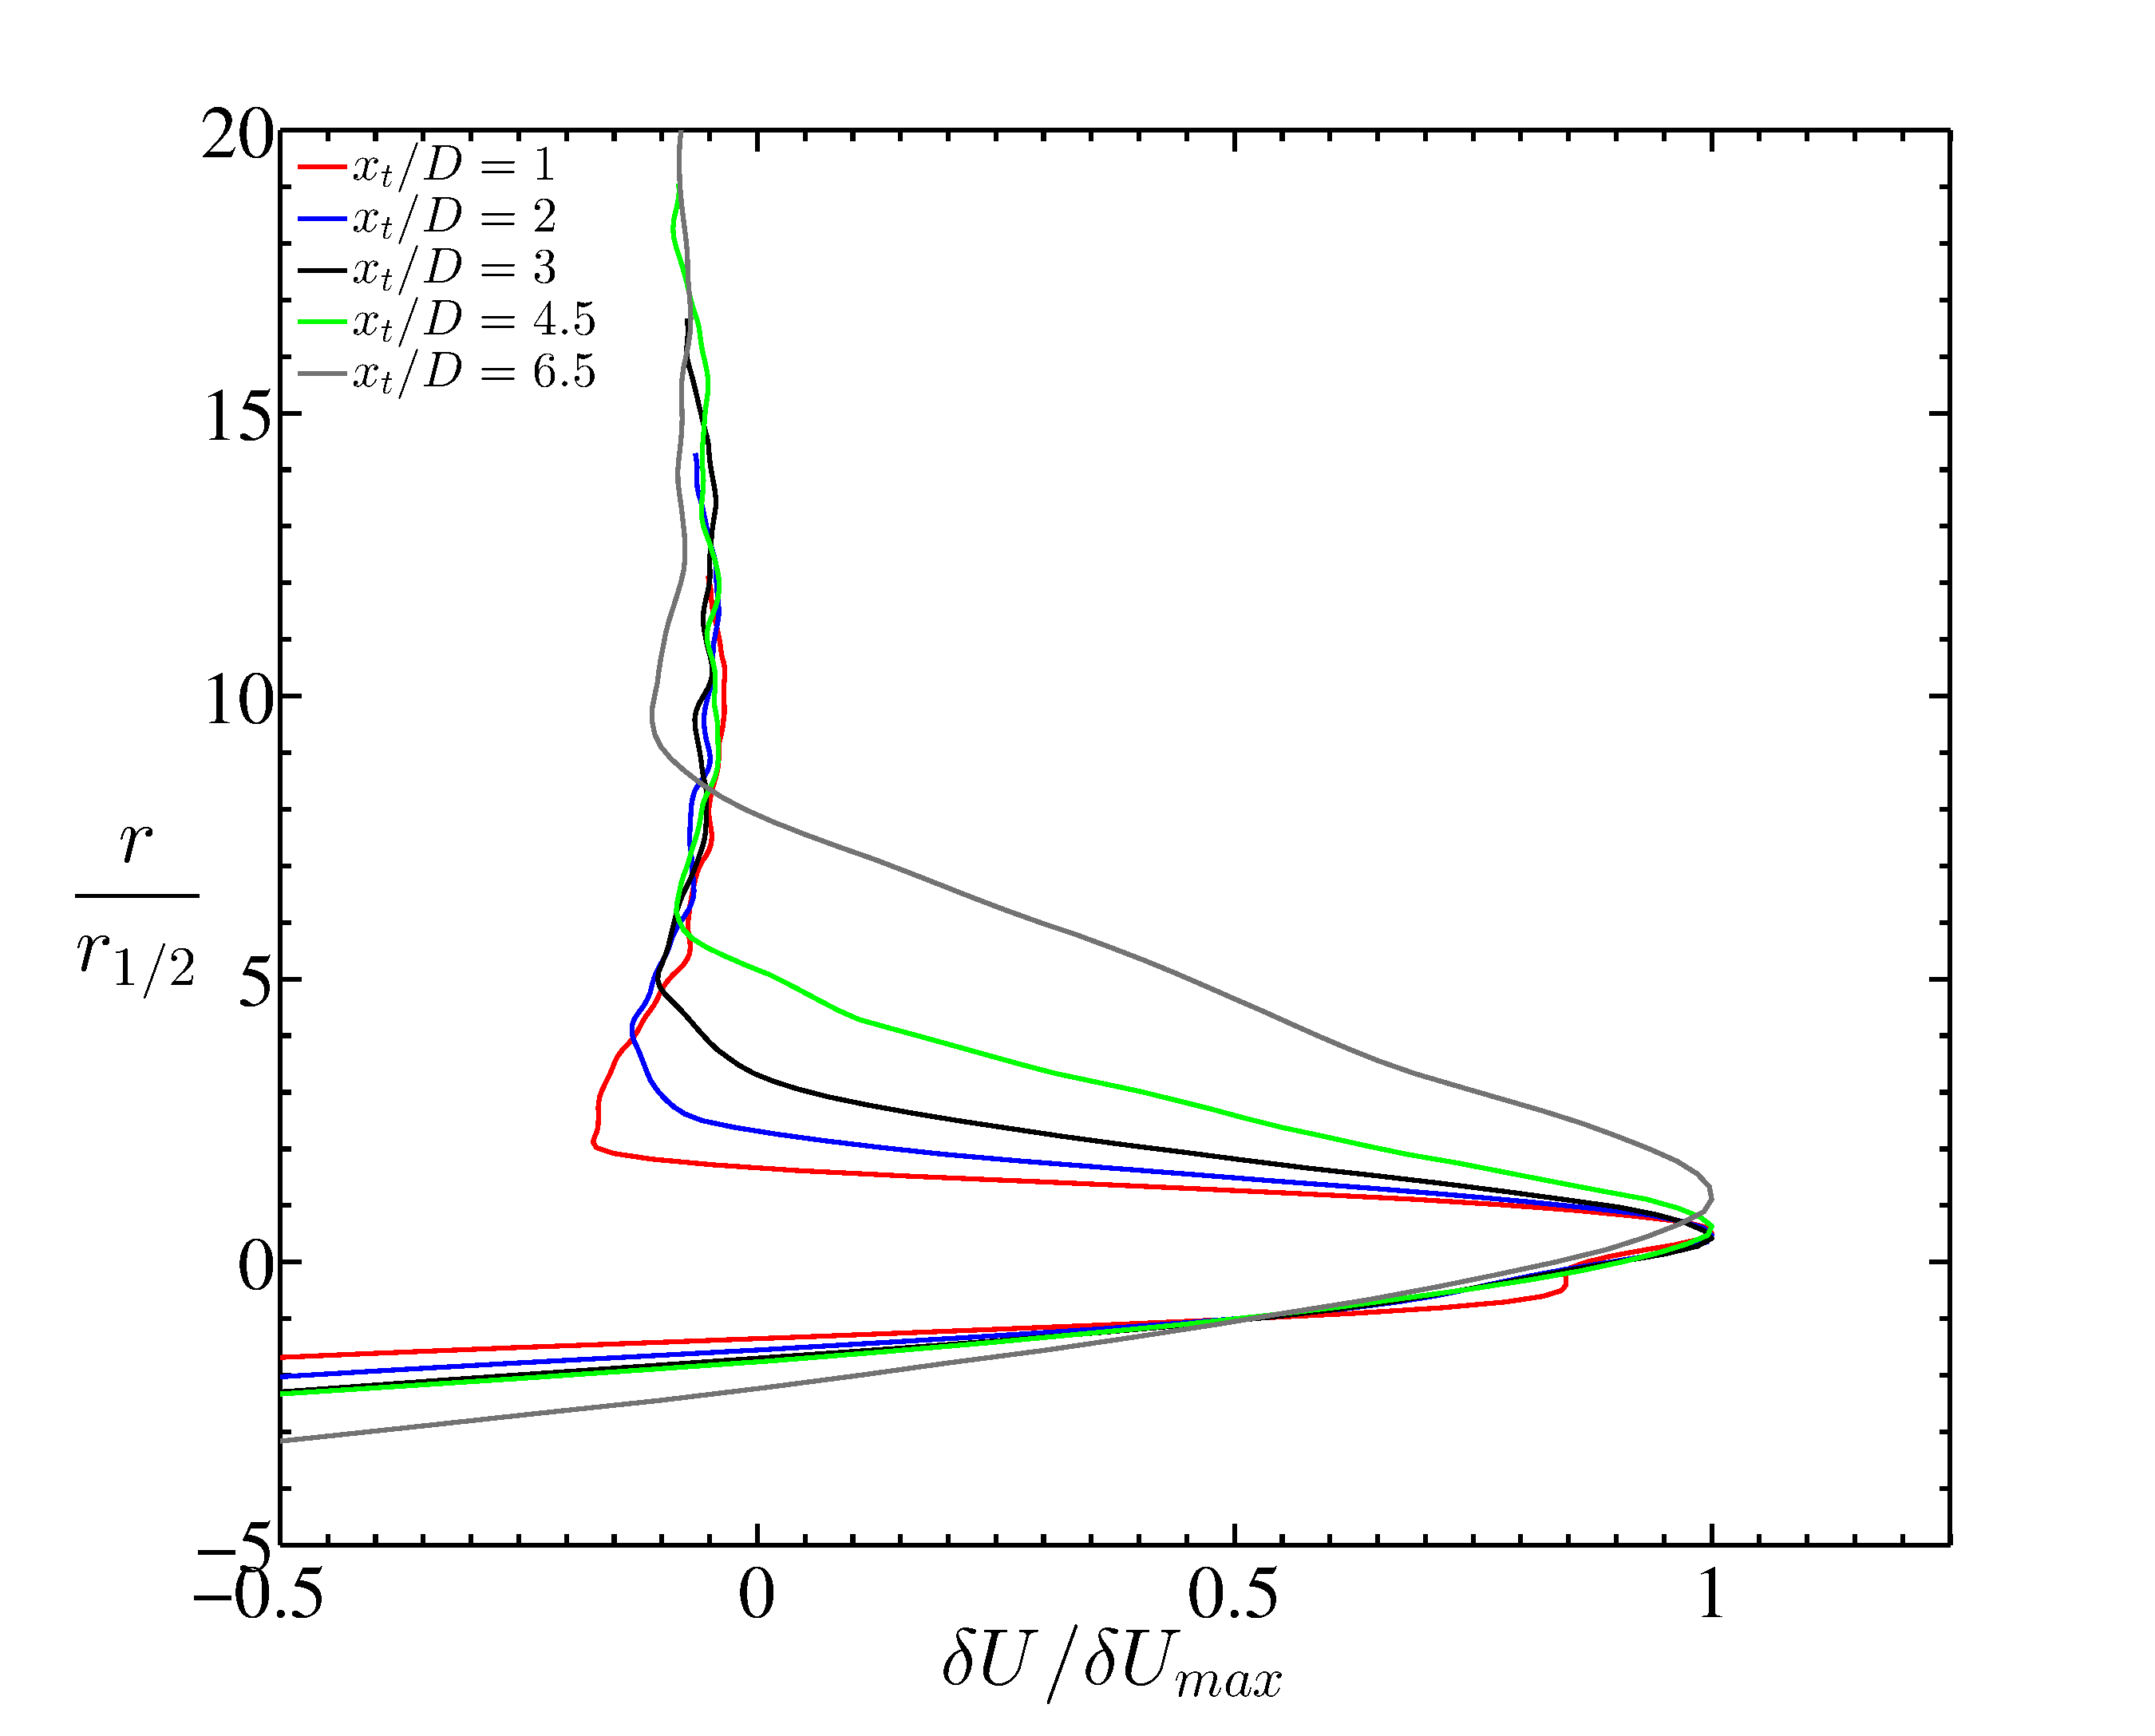
\includegraphics[width=\linewidth]{stats/similarity_velprof_Npts_zavg.pdf}
                \caption{}
                \label{fig:mean1}
        \end{subfigure}%
        \centering
        \begin{subfigure}[t]{0.5\textwidth}
                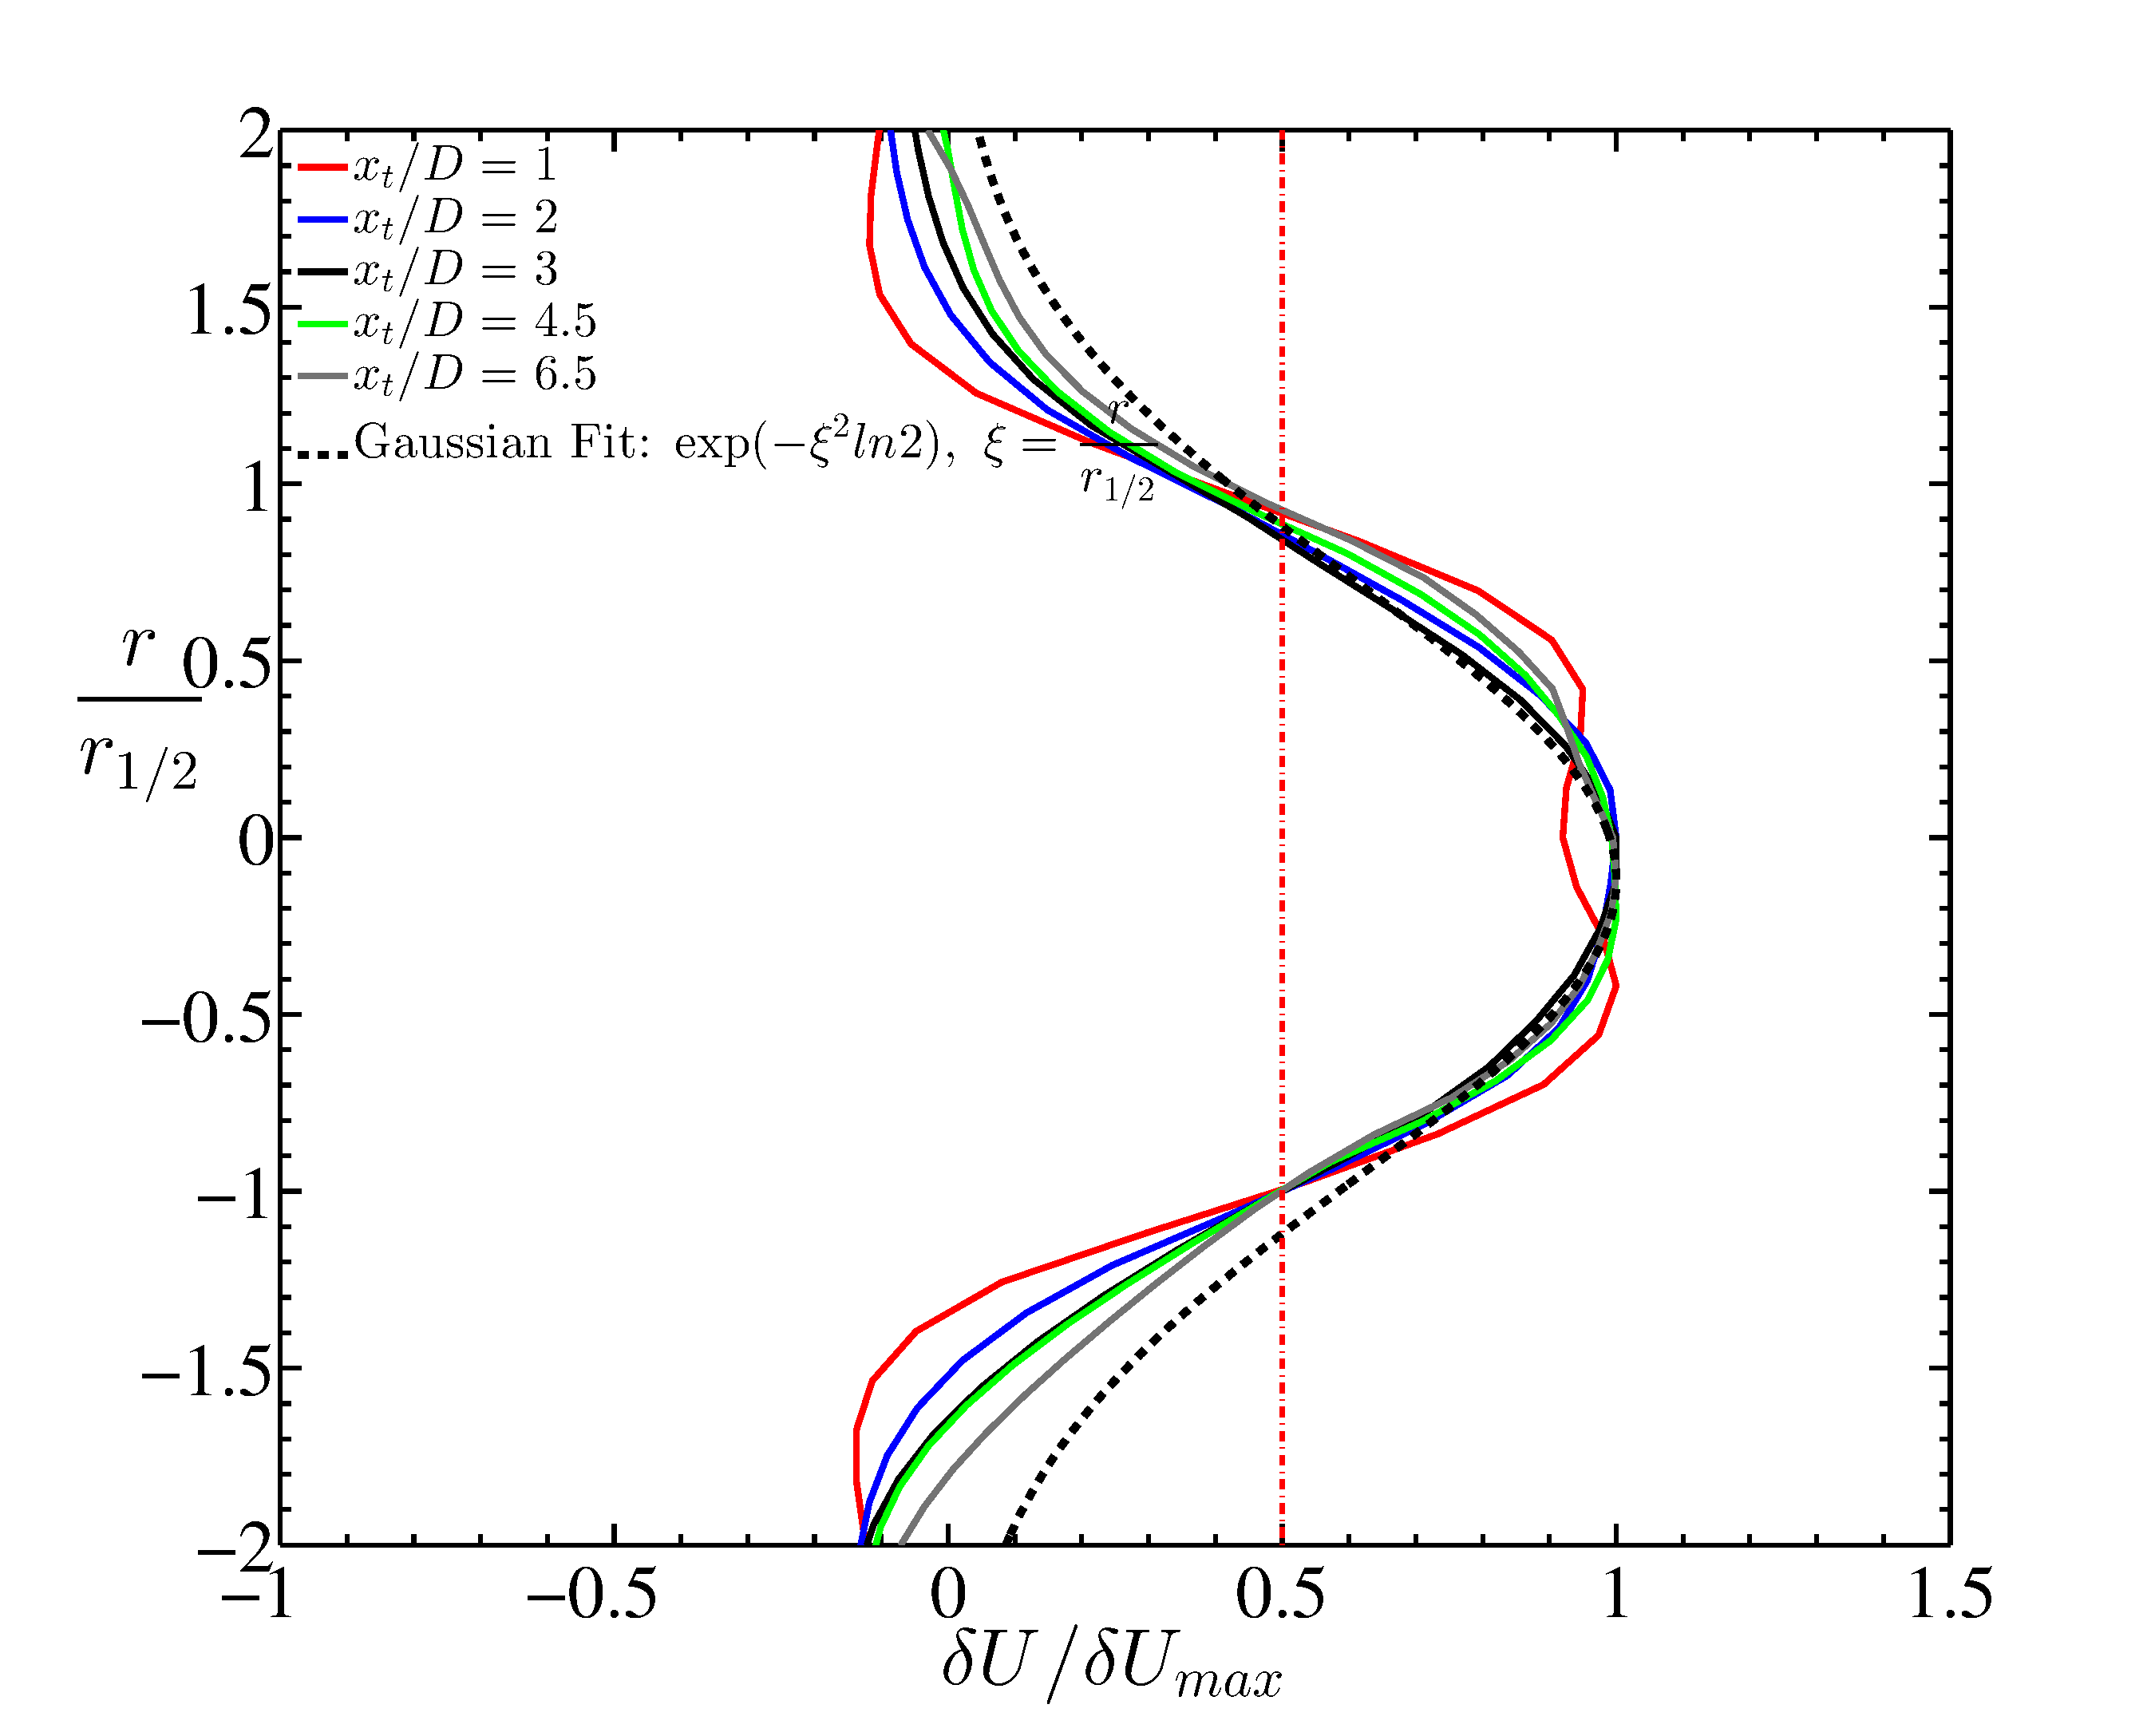
\includegraphics[width=\linewidth]{stats/similarity_velprof_Npts_2b.pdf}
                \caption{}
                \label{fig:mean2}
        \end{subfigure}
        \caption[Wake similarity laws]{Estimation of similarity scaling laws of normalized wake velocity deficit $\frac{\delta U}{\delta U_{max}}$ vs $r(x)/r_{1/2}$. (A) $xz$ plane (B) $xy$ plane} \label{fig:similarity}
\end{figure}
    
%--------------------stats figure ---------------------%
\begin{figure}
\centering
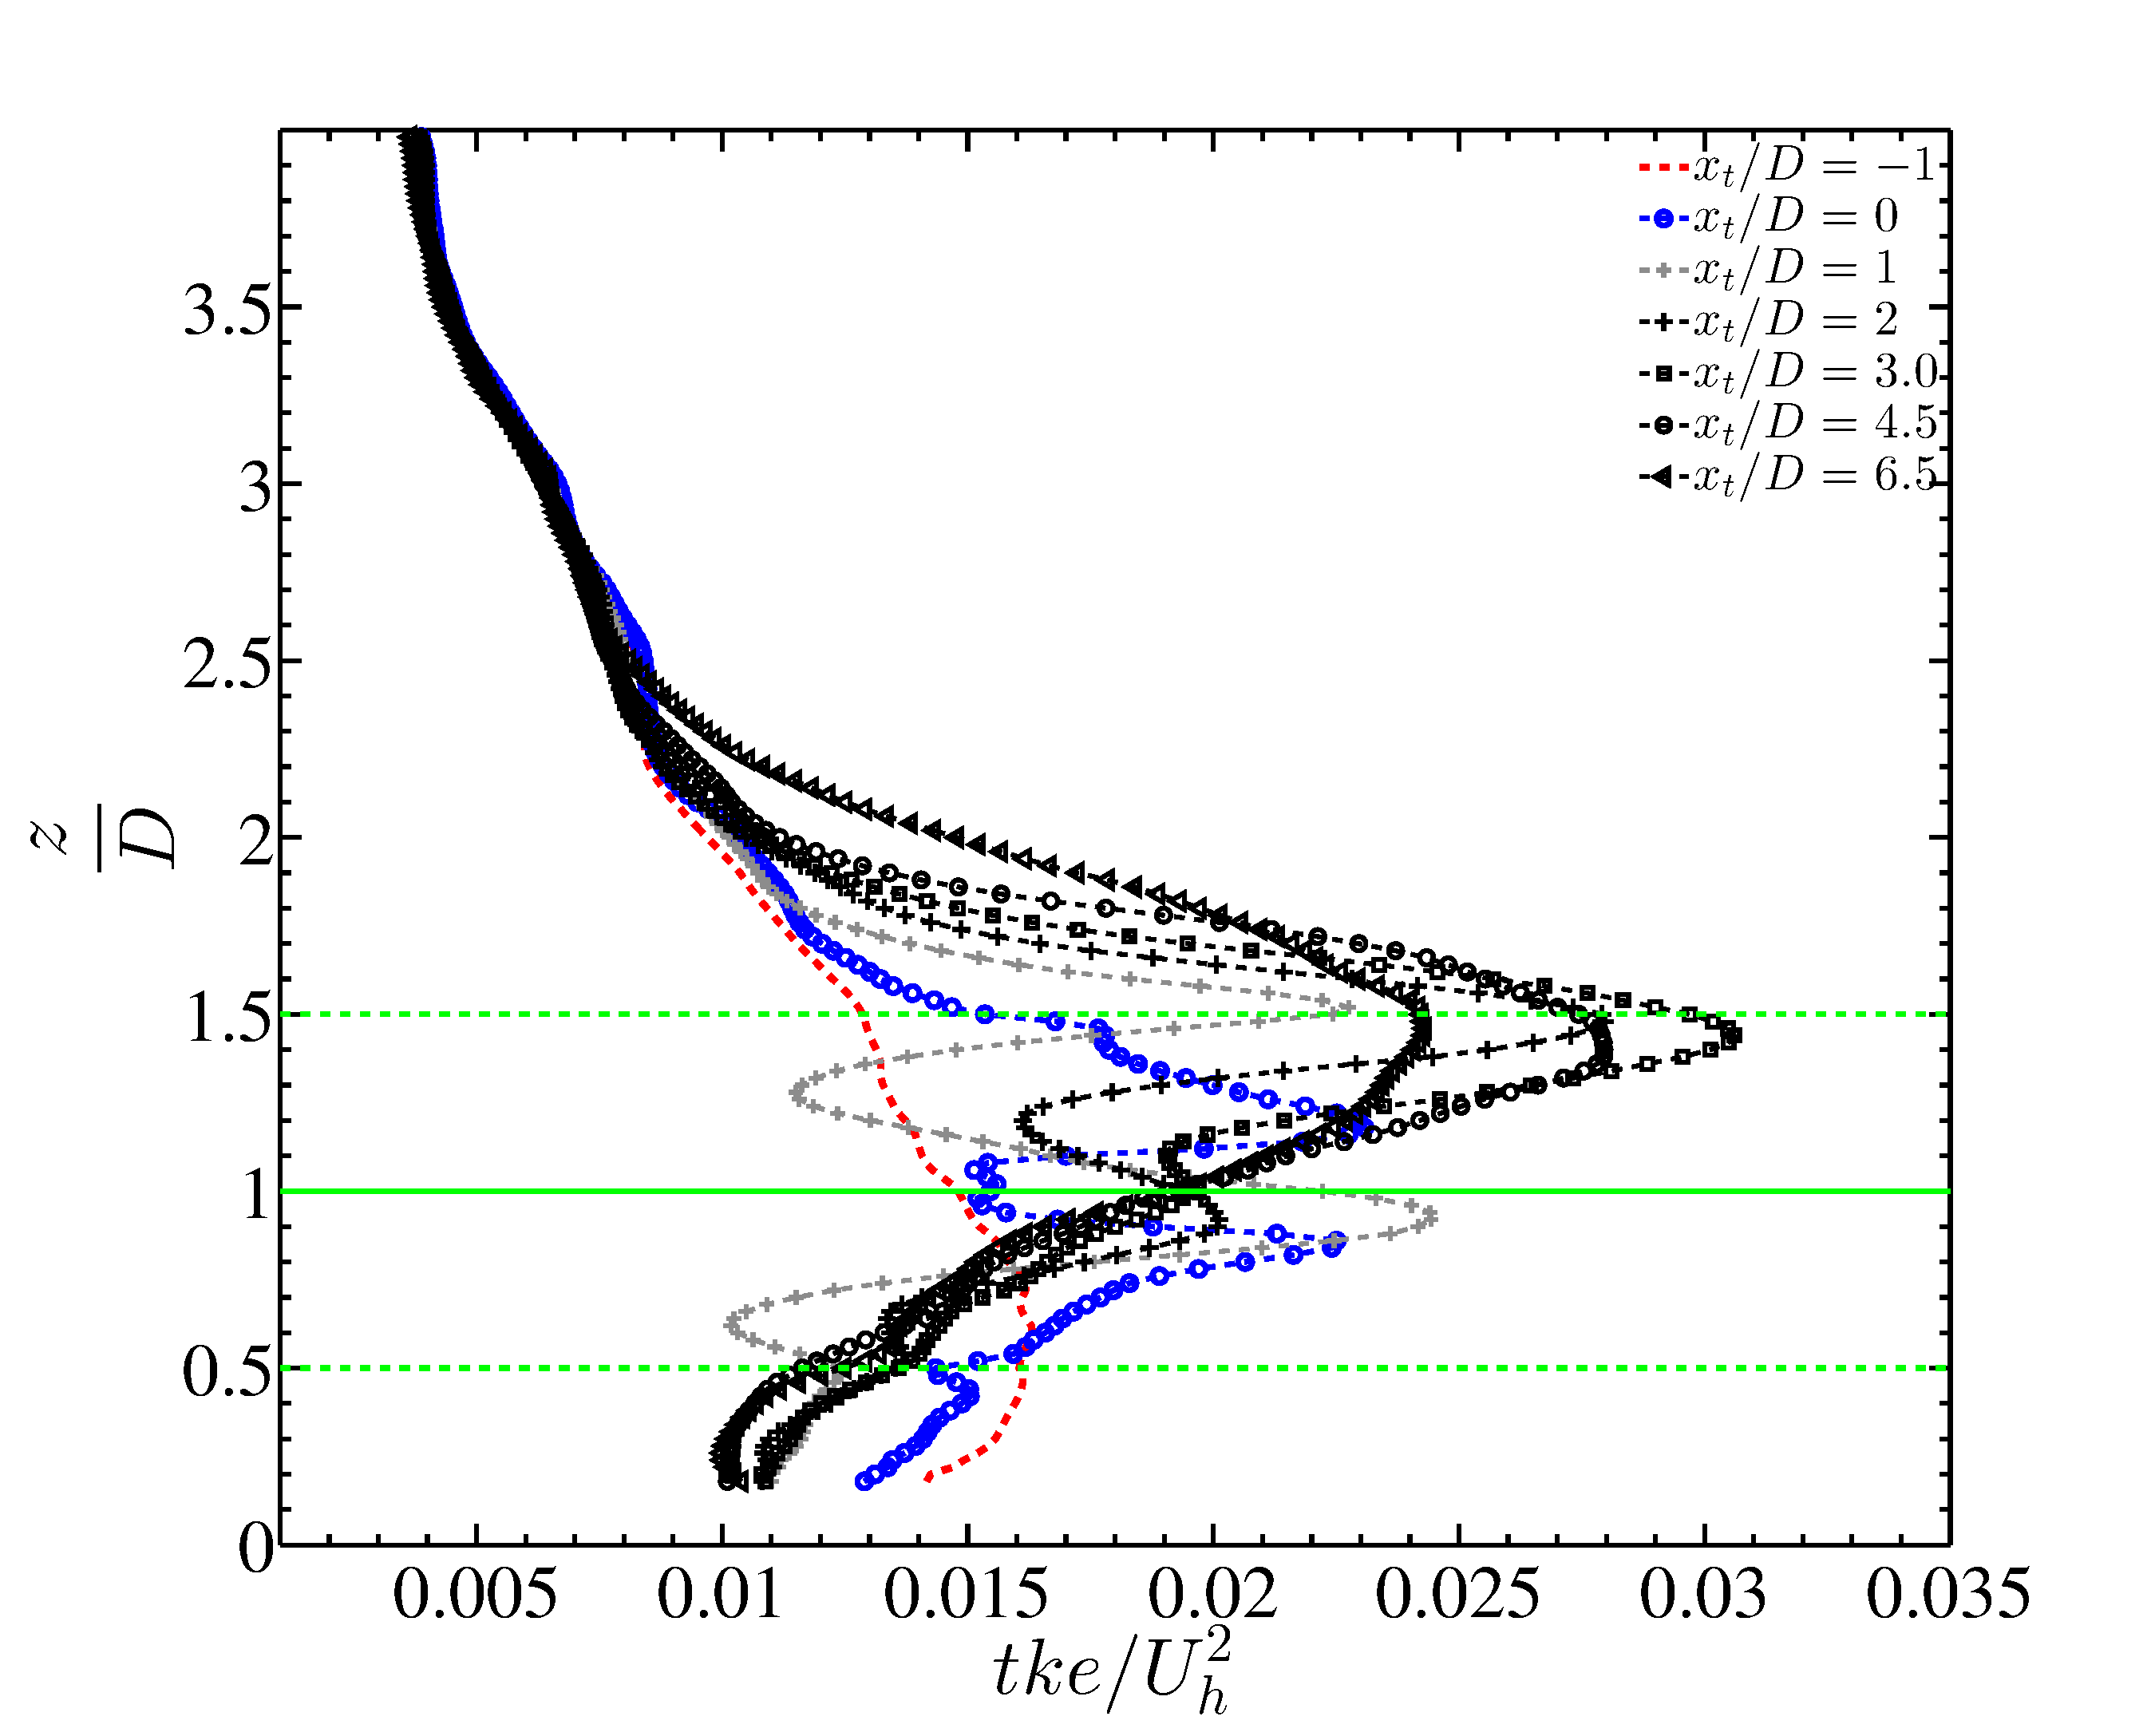
\includegraphics[width = 0.8\linewidth]{stats/tkeprof_3points_avg.pdf}
\caption[Mean tke at $x$ stations 1]{Temporally averaged mean turbulent kinetic energy at different streamwise $x$ stations. Profile averaged over the  3 spanwise points (center of turbine rotor).}\label{fig:tkestat1}
\end{figure}
\begin{figure}
\centering
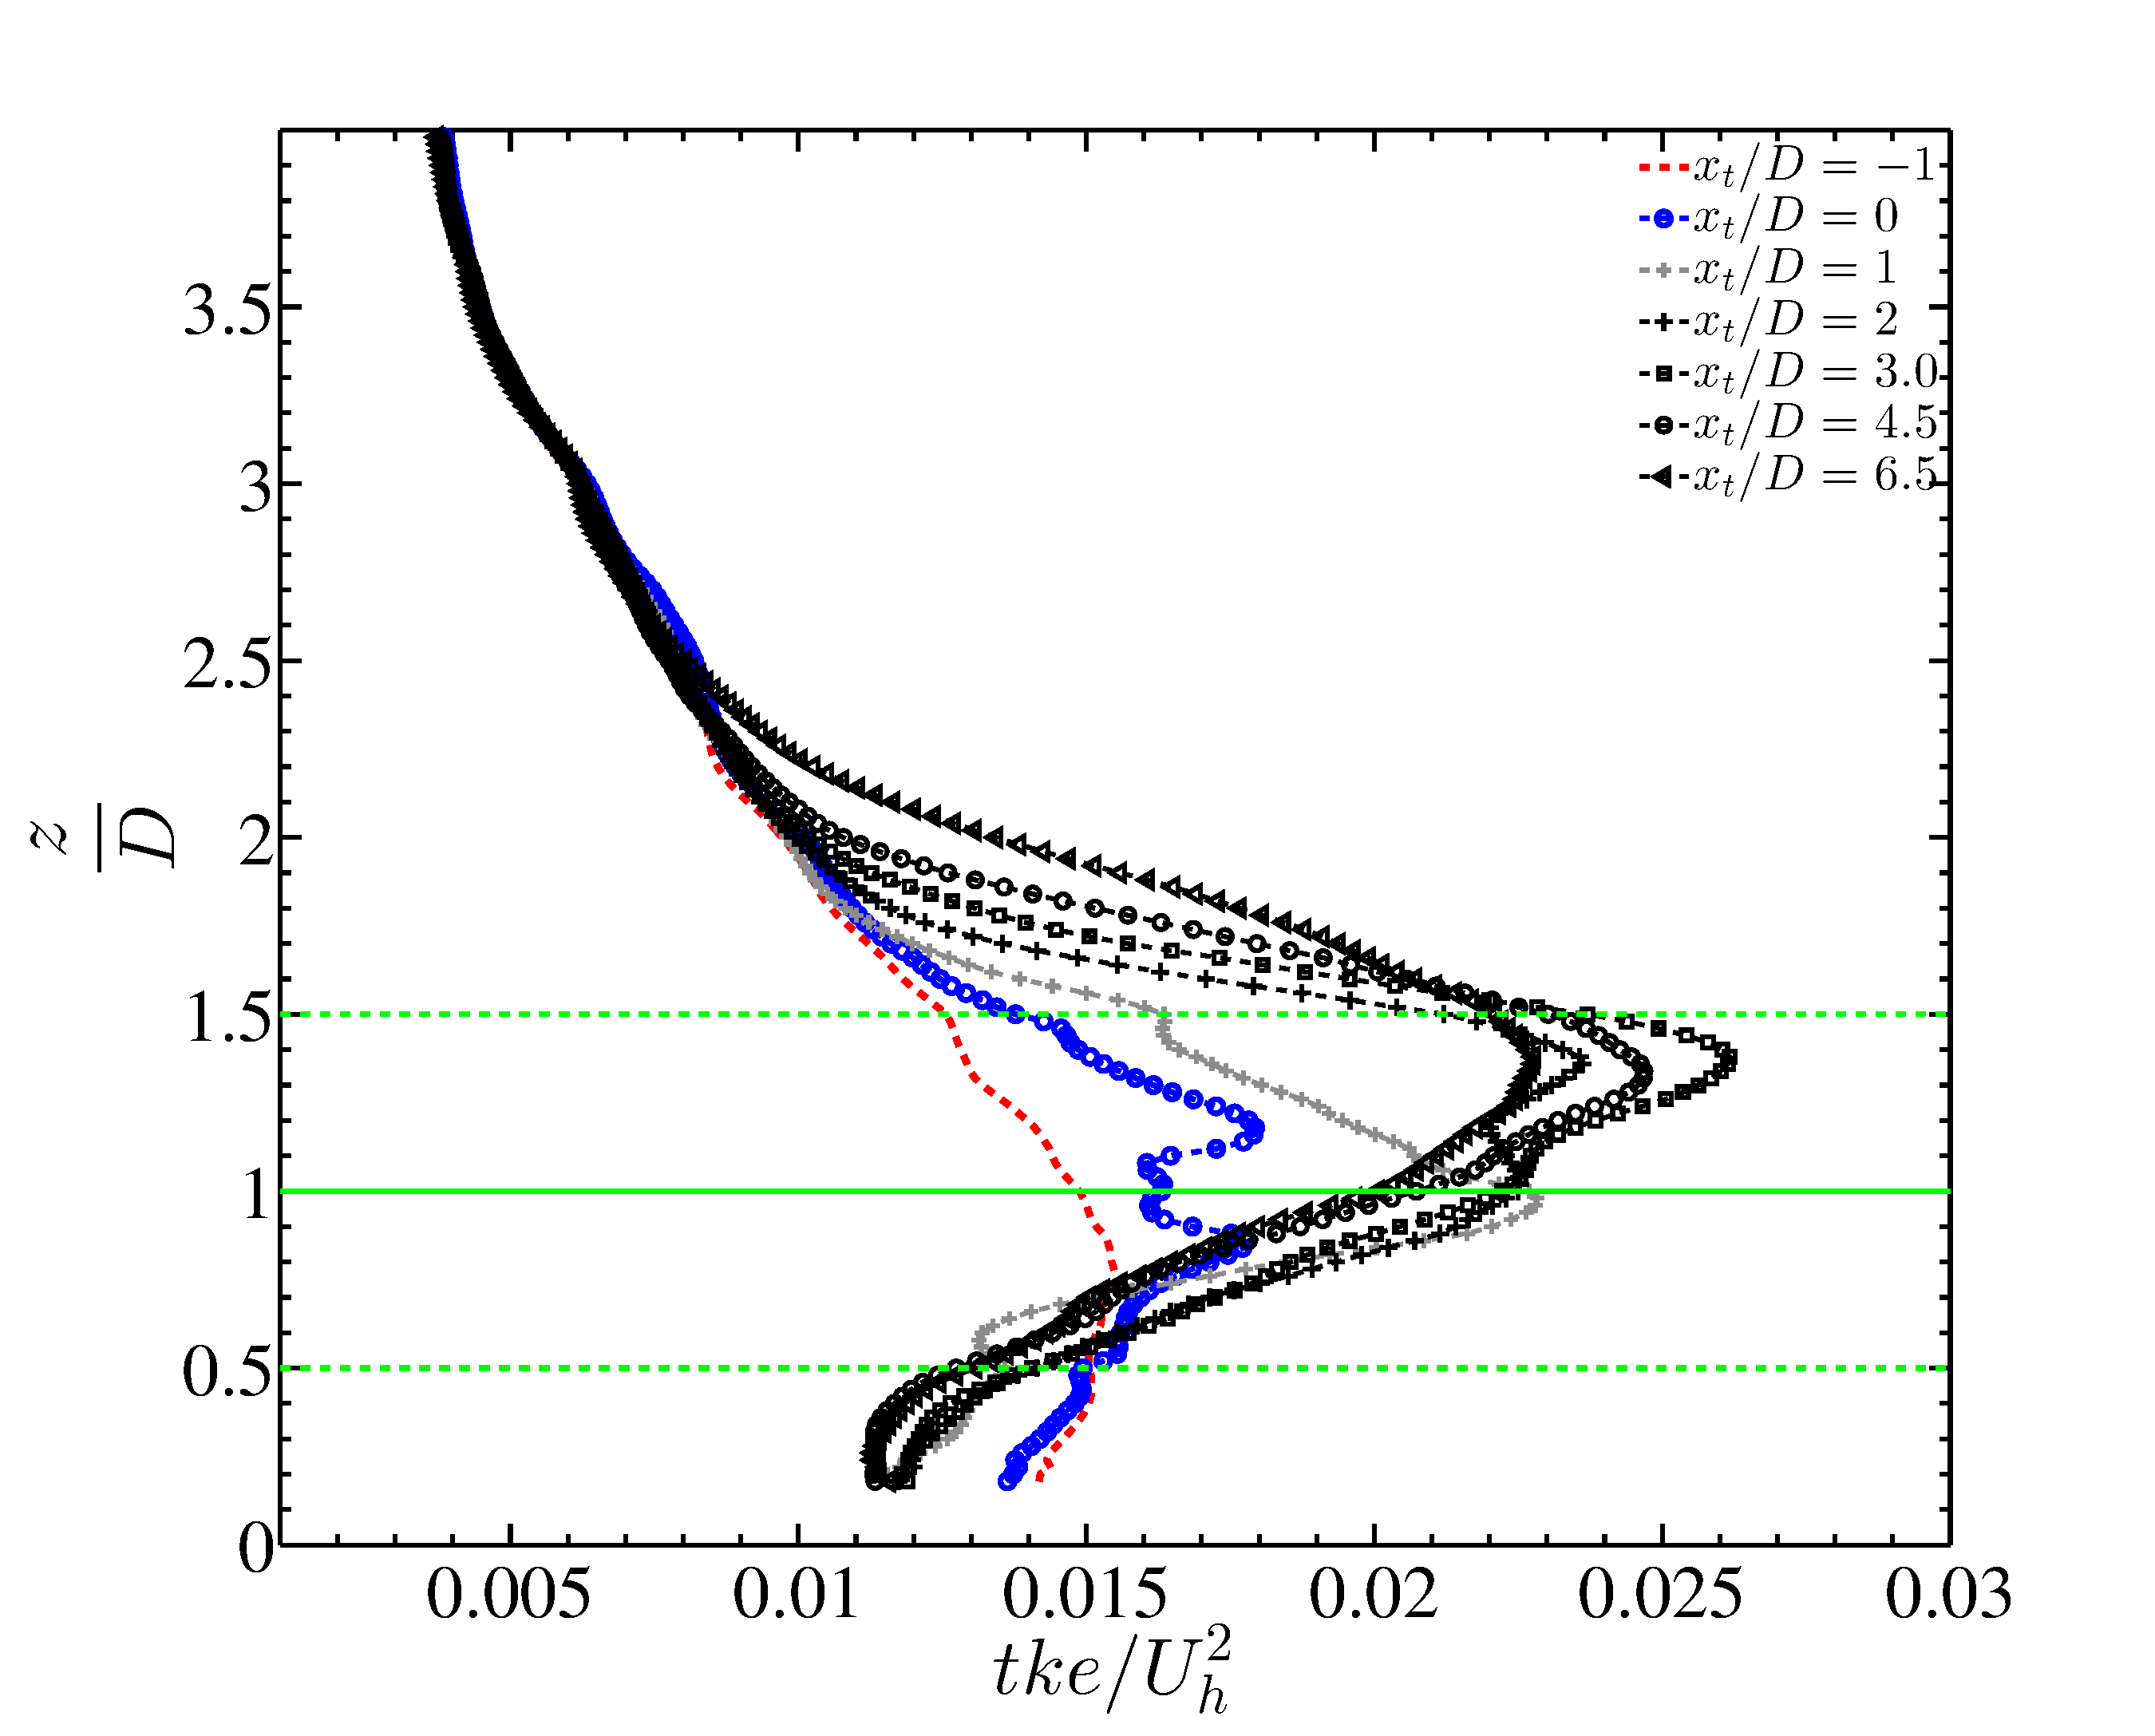
\includegraphics[width = 0.8\linewidth]{stats/tkeprof_9points_avg.pdf}
\caption[Mean tke at $x$ stations 2]{Temporally averaged mean turbulent kinetic energy at different streamwise $x$ stations. Profile averaged over the  9 spanwise points over 3 wind turbine rotor extents.}\label{fig:tkestat2}
\end{figure}
\begin{figure}
\centering
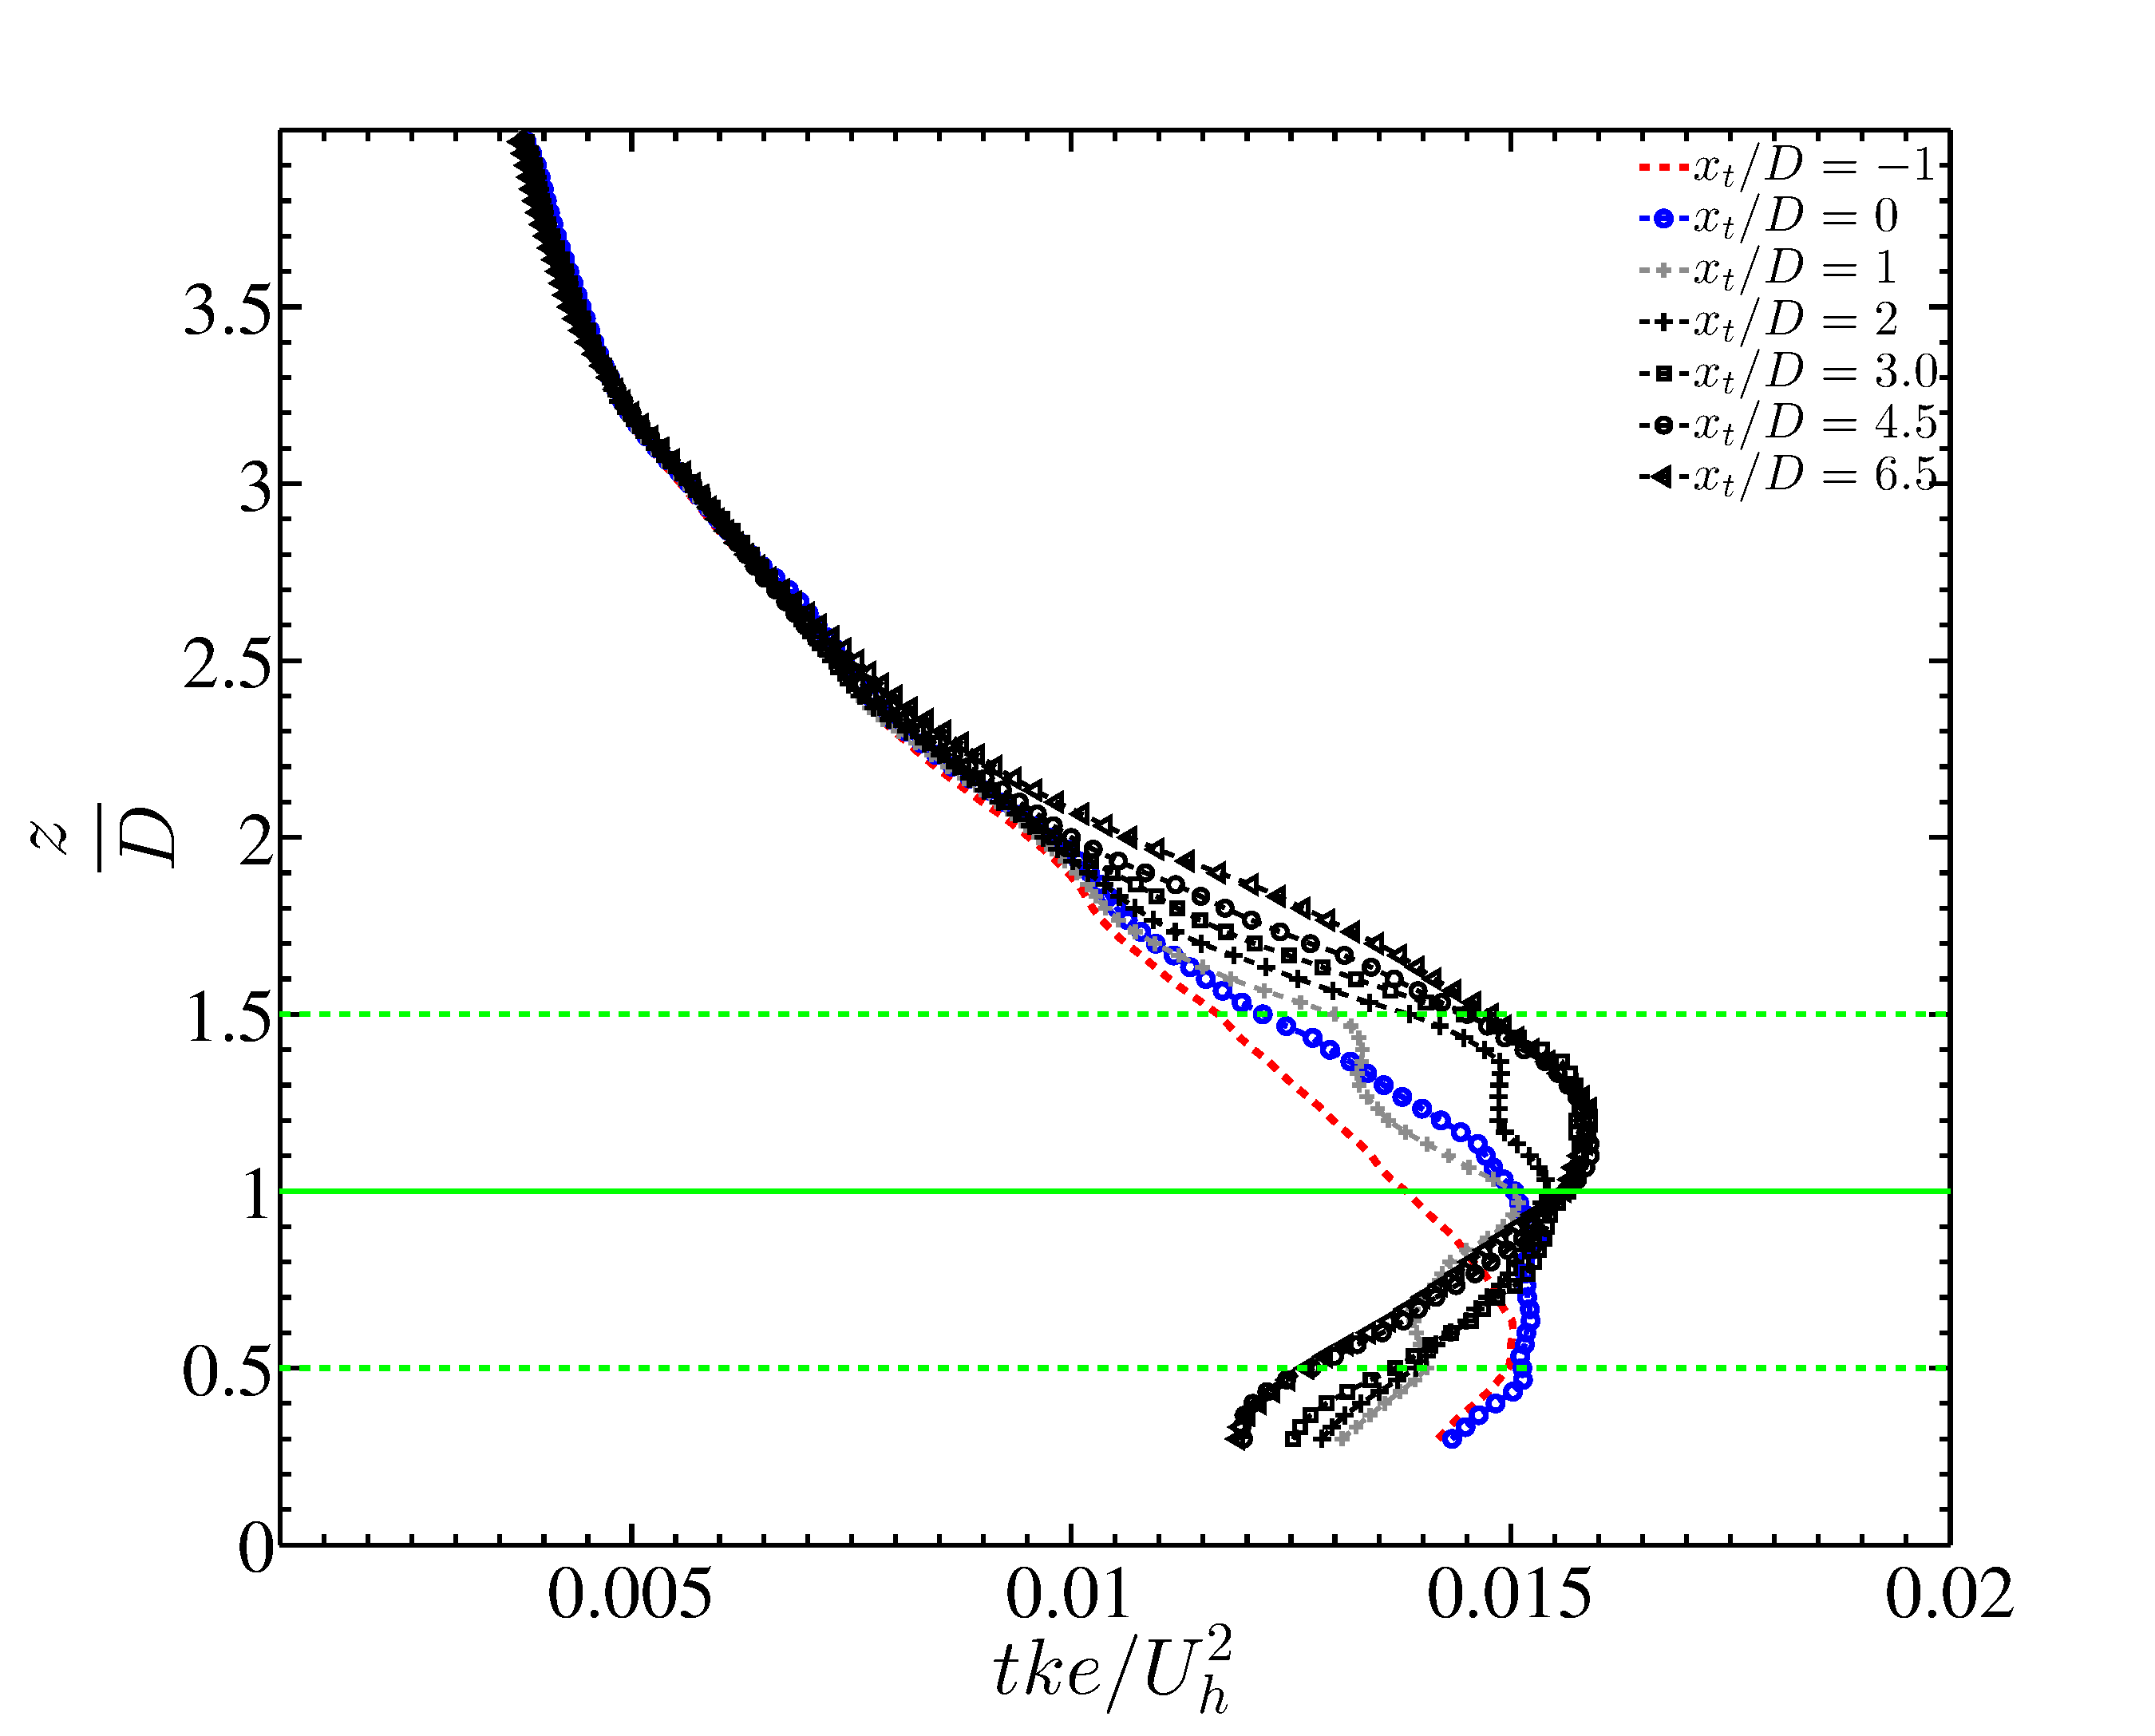
\includegraphics[width = 0.8\linewidth]{stats/tkeprof_Npoints_avg.pdf}
\caption[Mean tke at $x$ stations 3]{Temporally averaged mean turbulent kinetic energy at different streamwise $x$ stations. Profile averaged over the whole spanwise domain.}\label{fig:tkestat3}
\end{figure}

%--------------fluctuations stats figure---------------------%
\begin{figure}
\centering
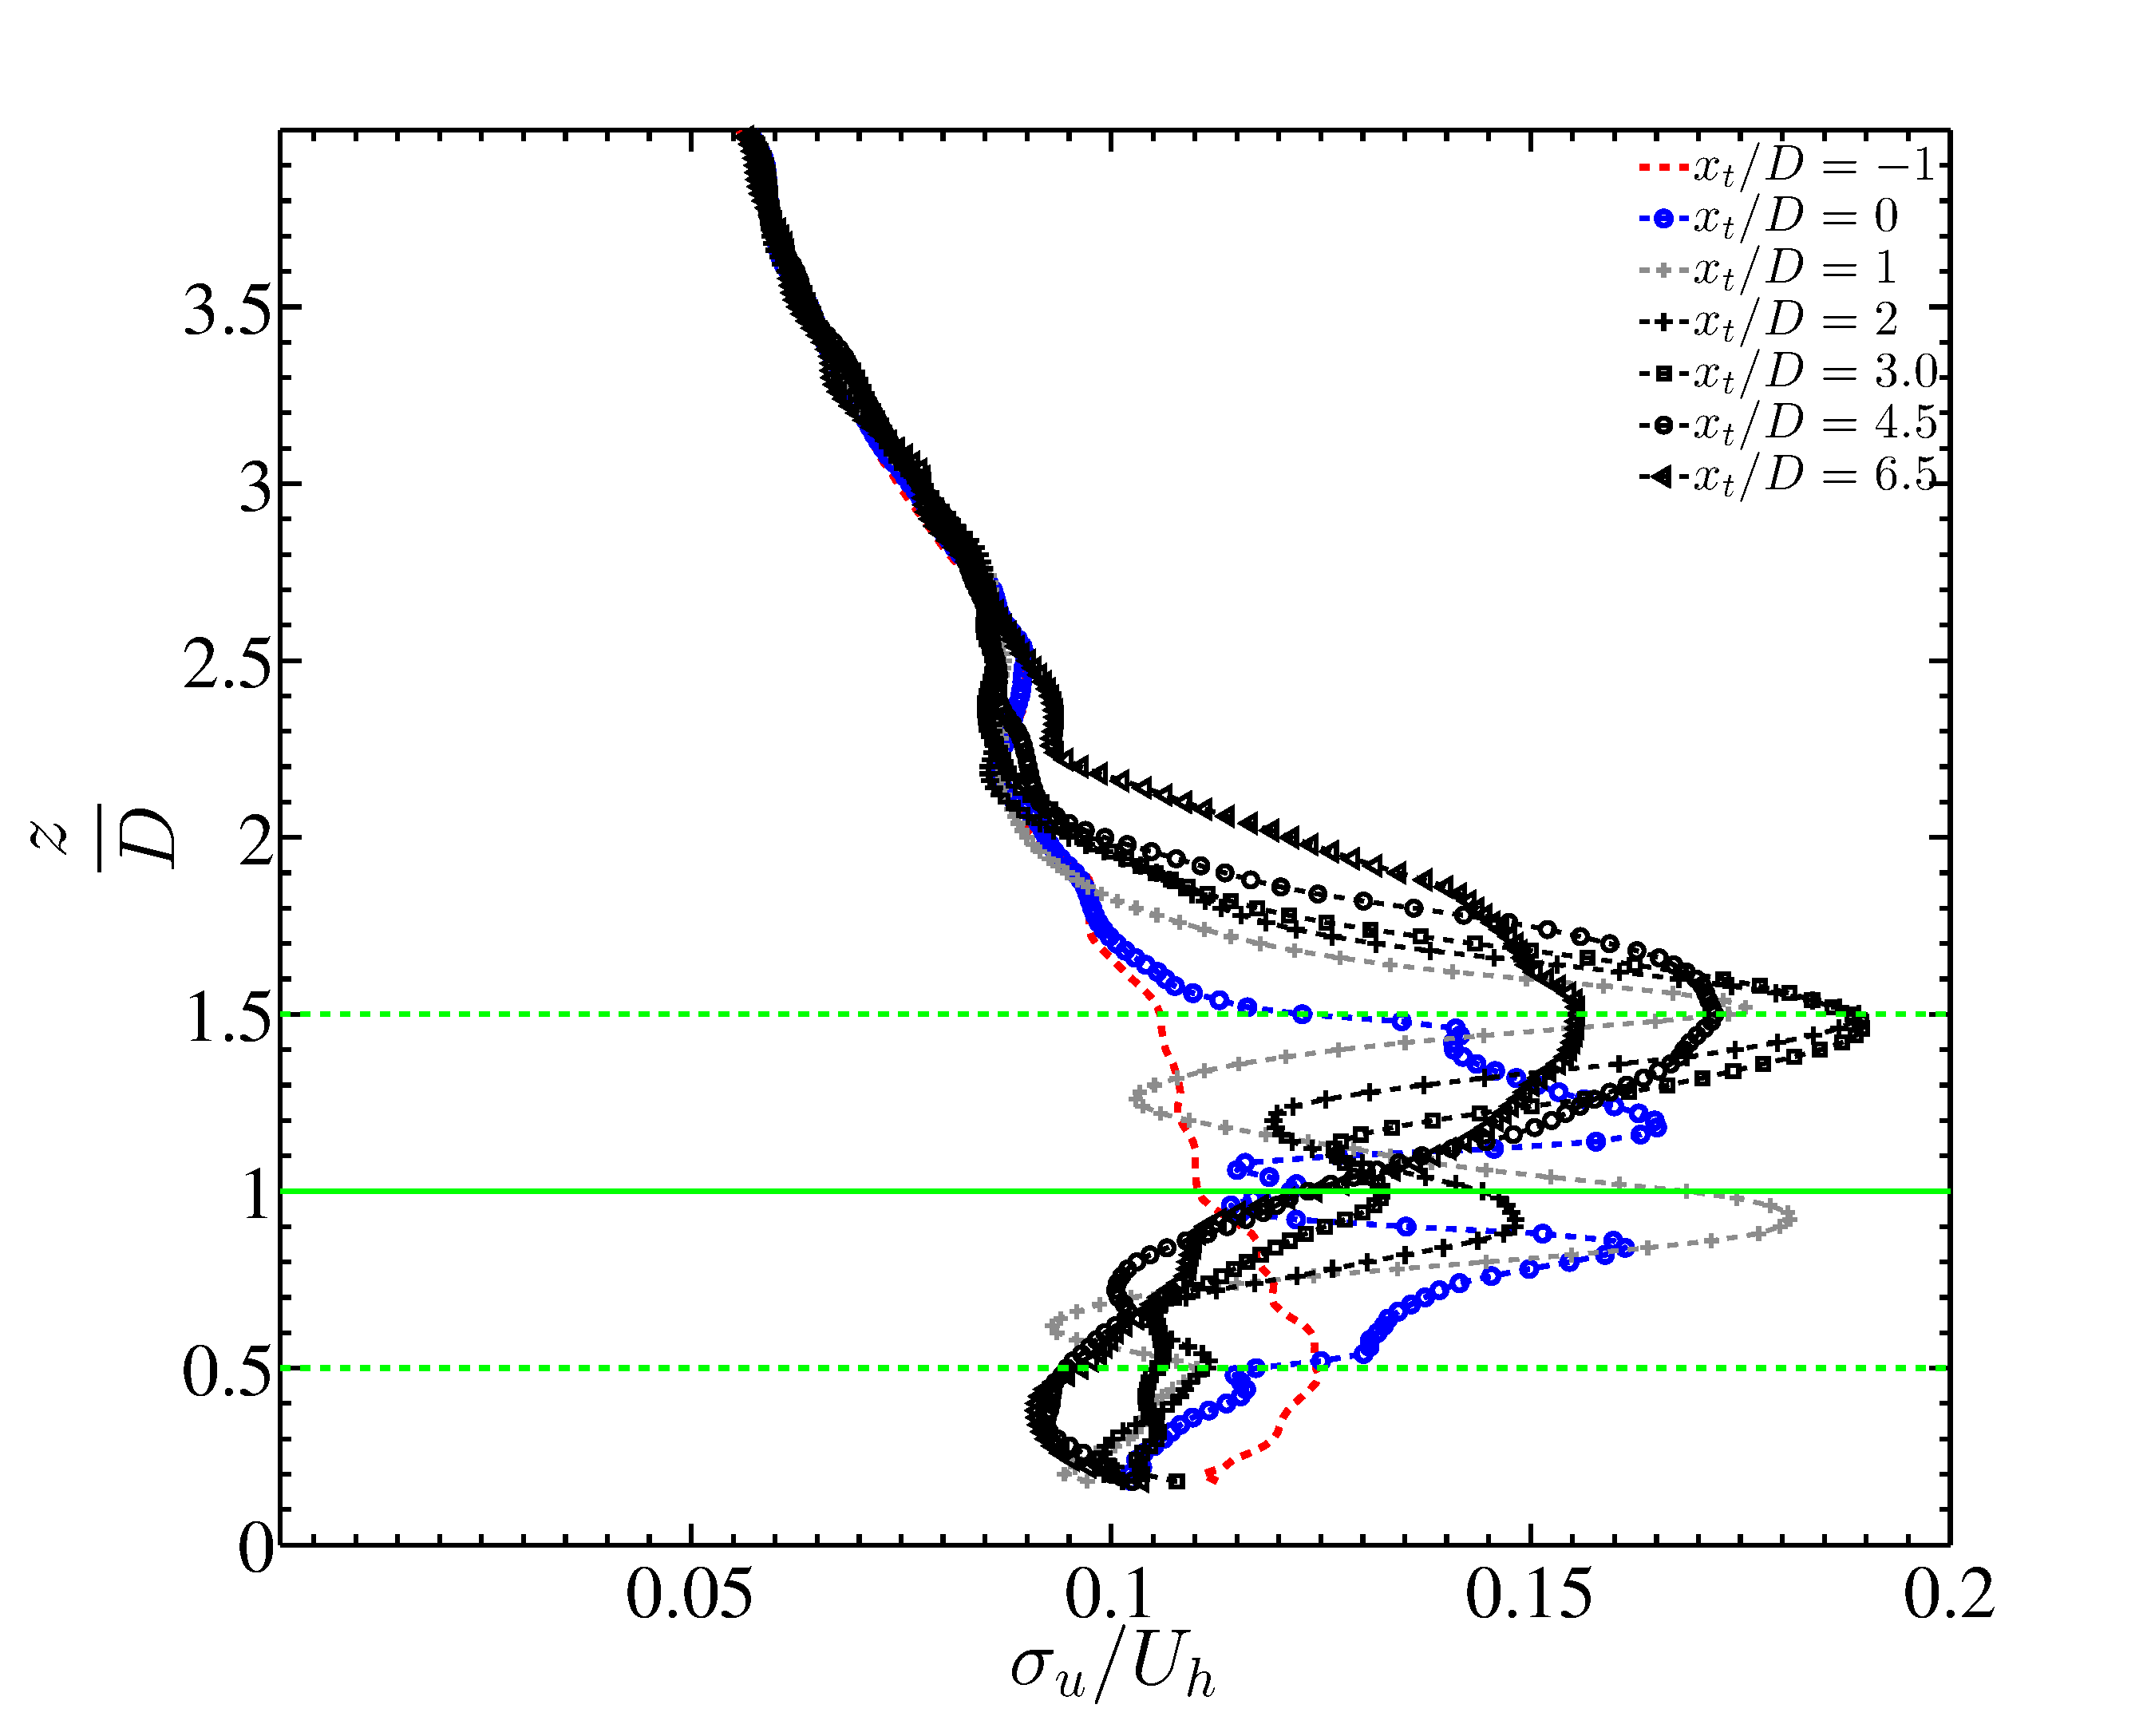
\includegraphics[width = 0.8\linewidth]{stats/ufluc_3points_avg.pdf}
\caption[Mean $\sigma_{u}$ at $x$ stations 1]{Temporally averaged streamwise turbulent intensity at different streamwise $x$ stations. Profile averaged over the  3 spanwise points (center of turbine rotor).}\label{fig:ustat1}
\end{figure}
\begin{figure}
\centering
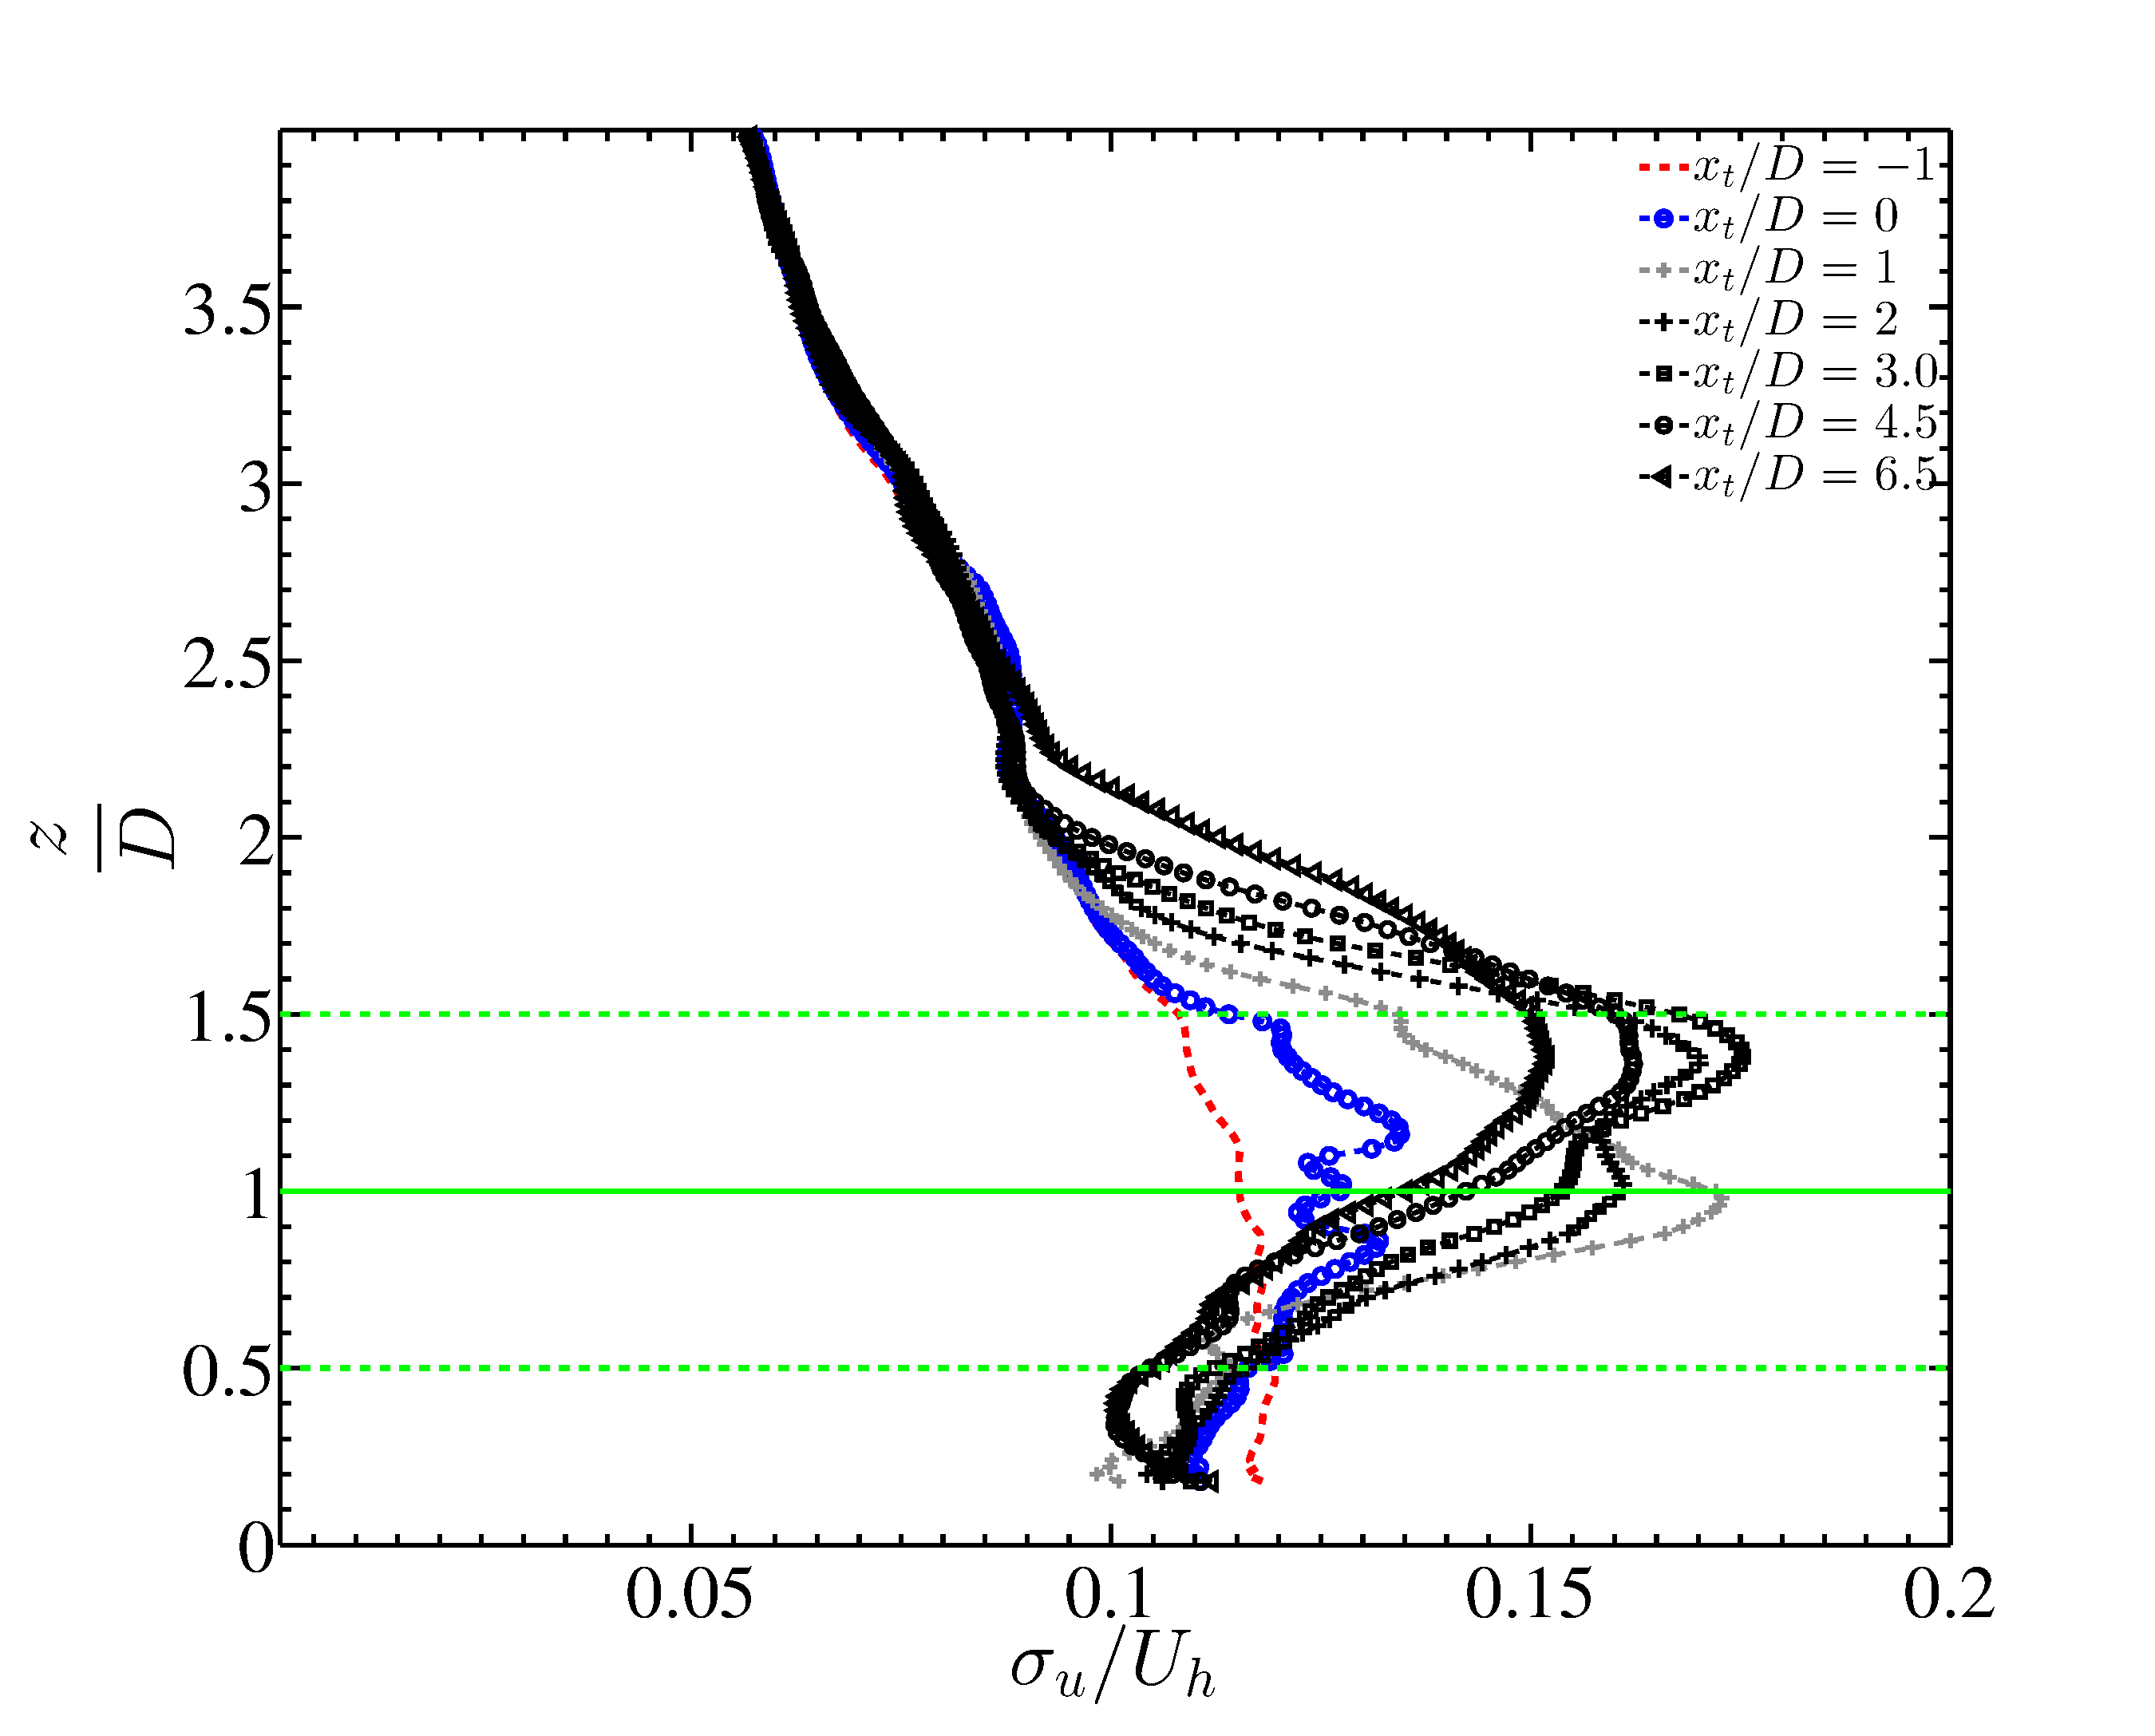
\includegraphics[width = 0.8\linewidth]{stats/ufluc_9points_avg.pdf}
\caption[Mean $\sigma_{u}$ at $x$ stations 2]{Temporally averaged mean streamwise turbulent intensity at different streamwise $x$ stations. Profile averaged over the  9 spanwise points over 3 wind turbine rotor extents.}\label{fig:ustat2}
\end{figure}
\begin{figure}
\centering
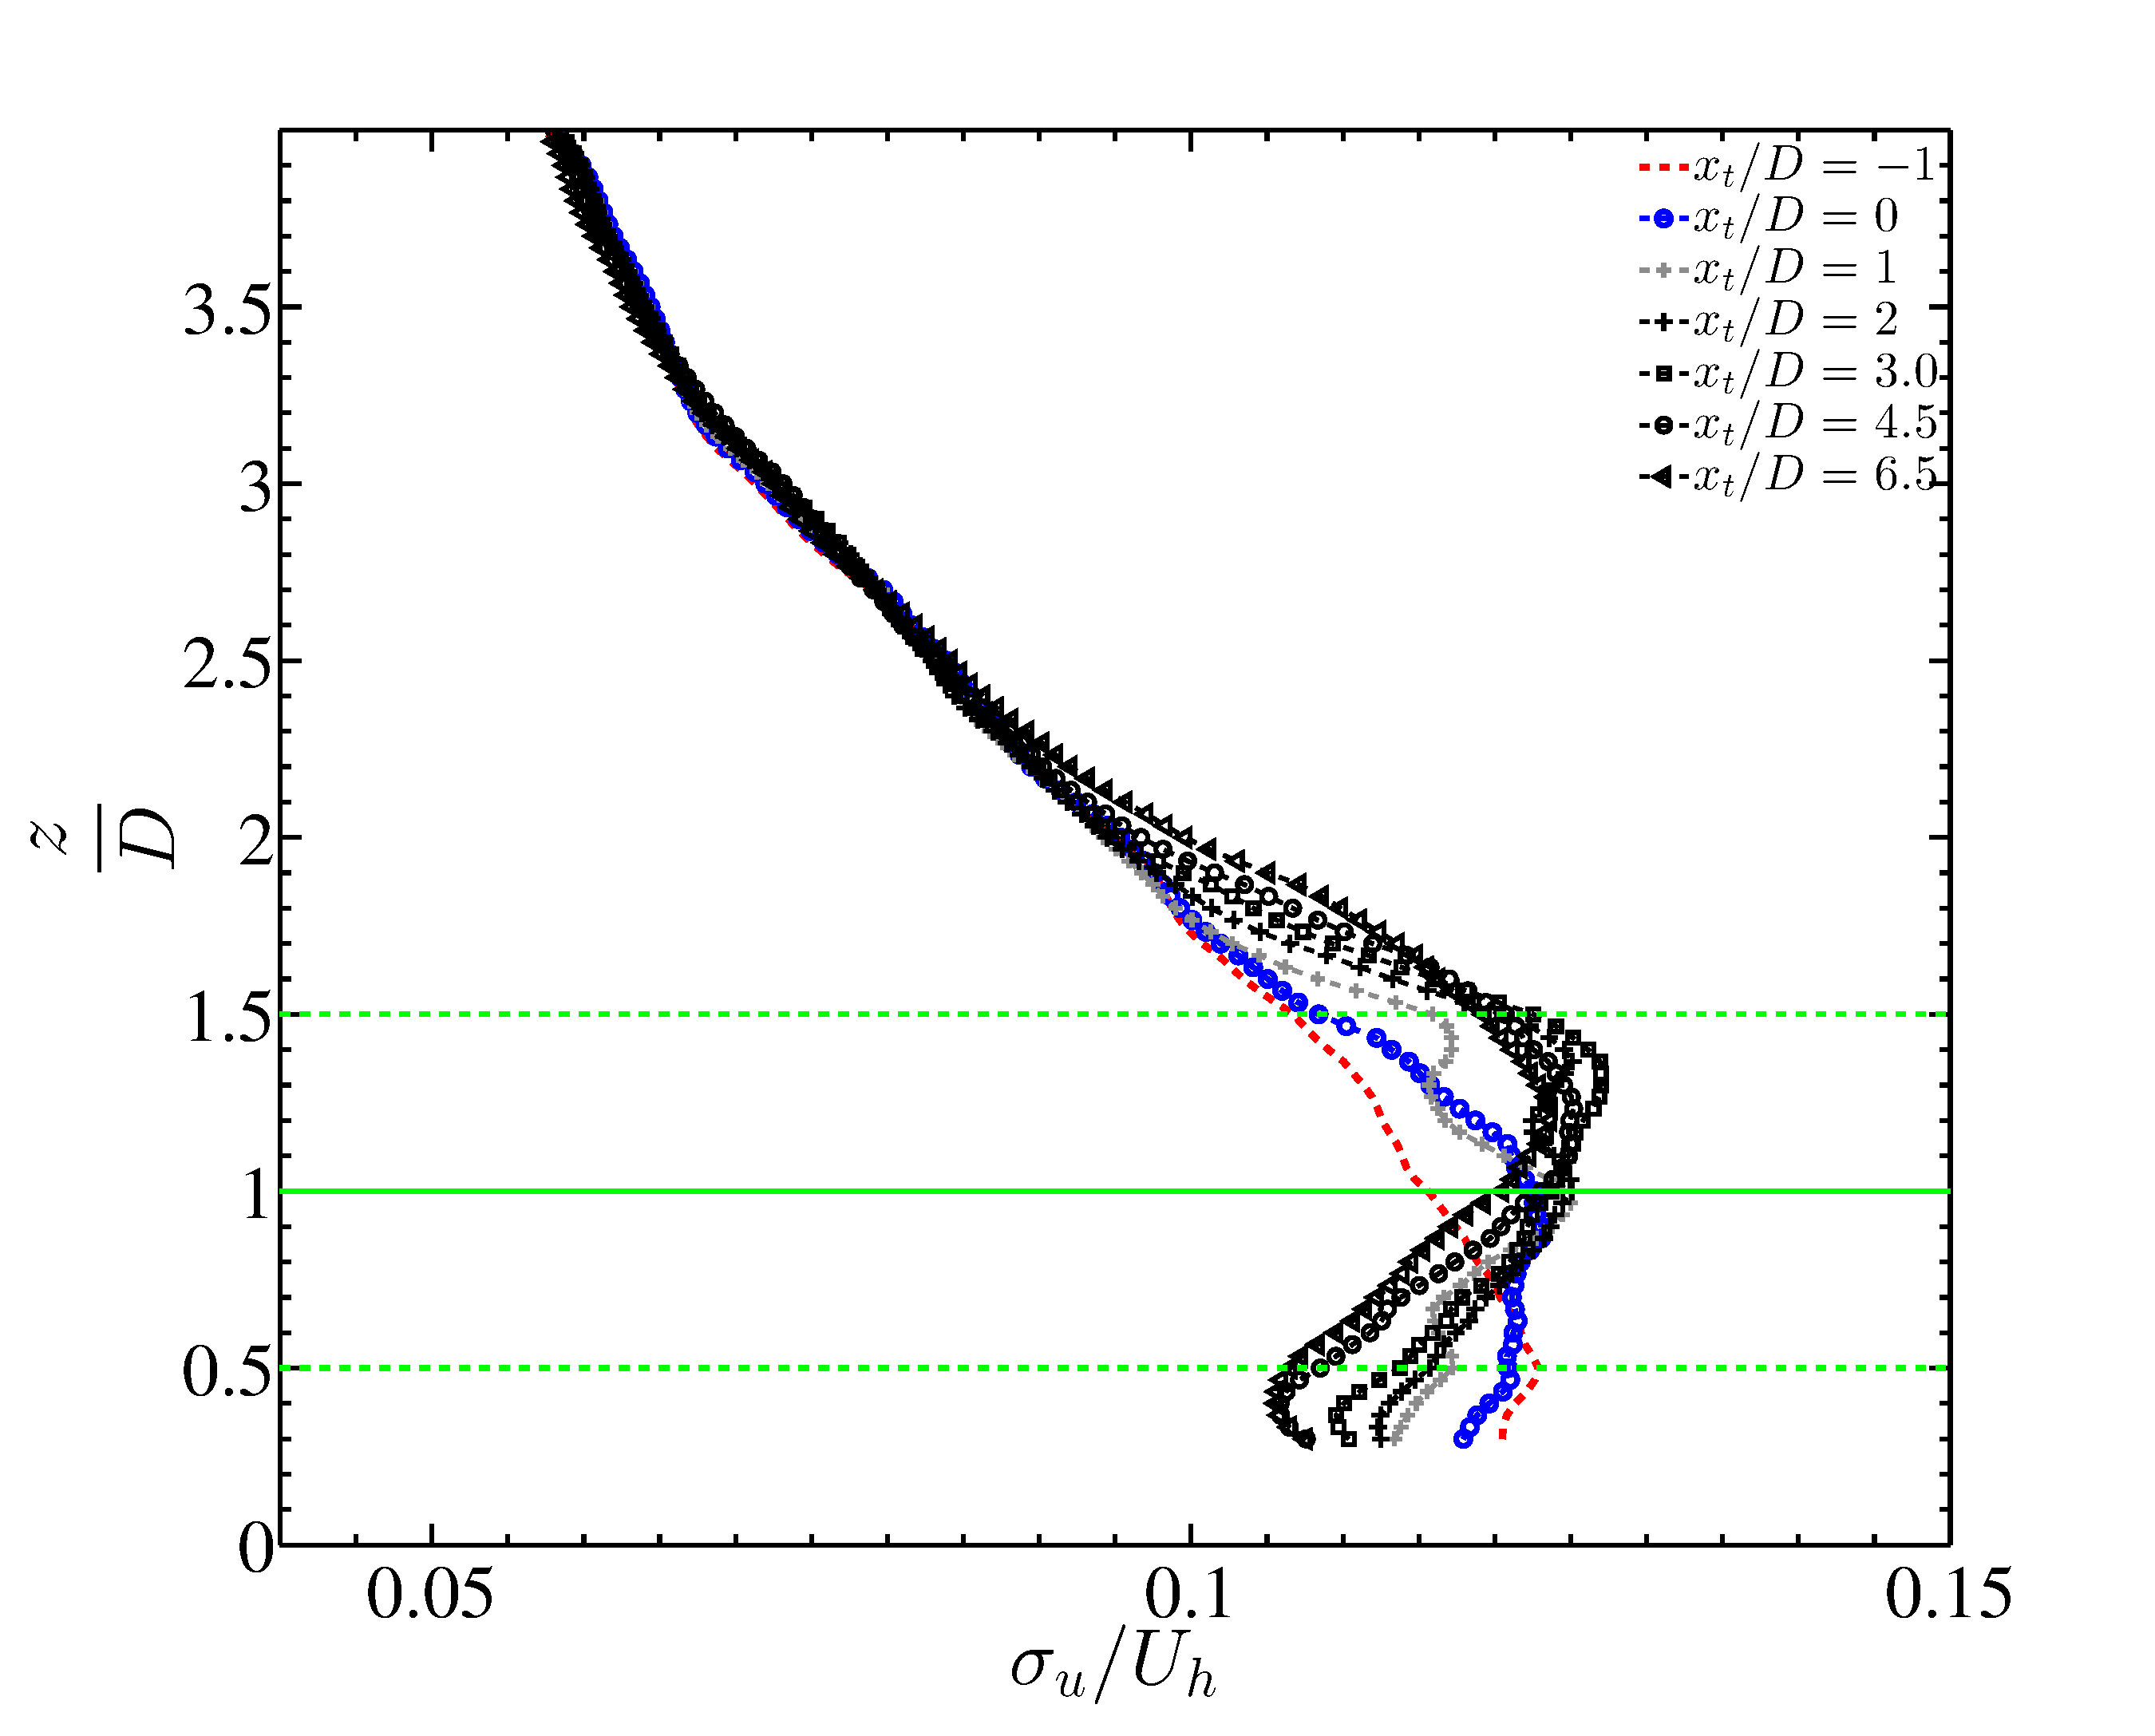
\includegraphics[width = 0.8\linewidth]{stats/ufluc_Npoints_avg.pdf}
\caption[Mean $\sigma_{u}$ at $x$ stations 3]{Temporally averaged mean streamwise turbulent intensity at different streamwise $x$ stations. Profile averaged over the whole spanwise domain.}\label{fig:ustat3}
\end{figure}
%---------------------------------------------------------------------------%
\begin{figure}
\centering
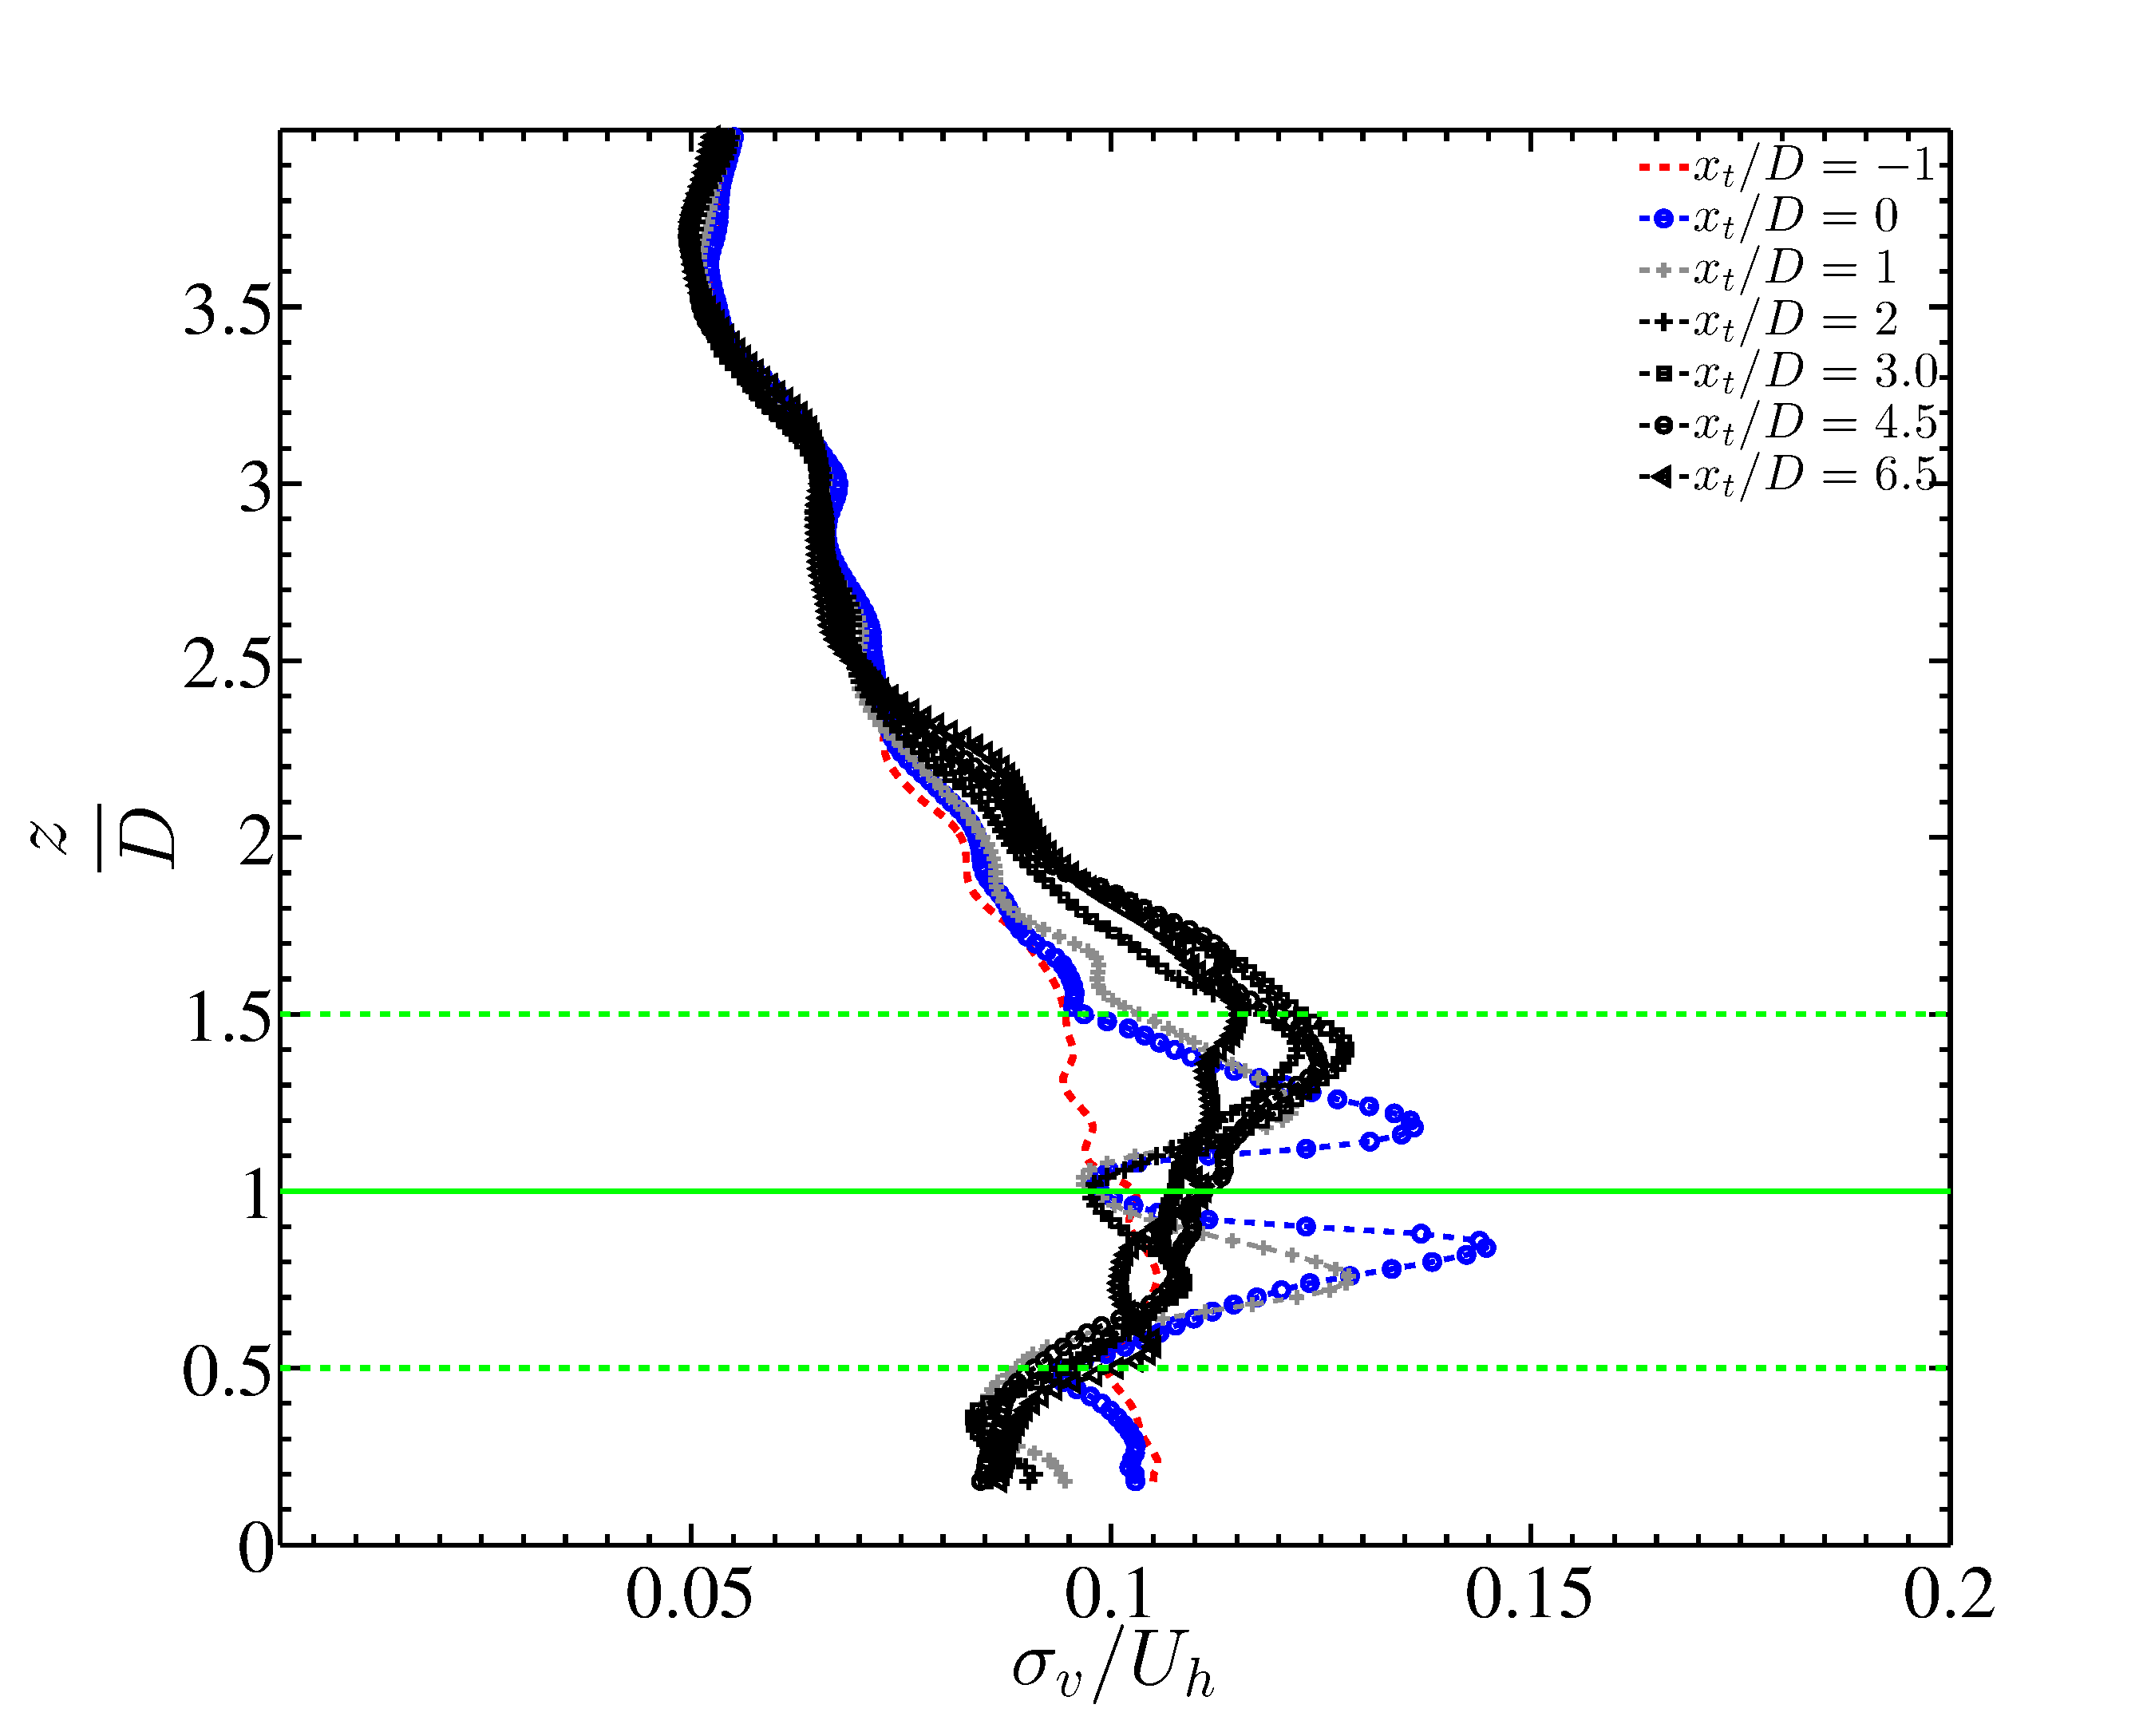
\includegraphics[width = 0.8\linewidth]{stats/vfluc_3points_avg.pdf}
\caption[Mean $\sigma_{v}$ at $x$ stations 1]{Temporally averaged spanwise turbulent intensity at different streamwise $x$ stations. Profile averaged over the  3 spanwise points (center of turbine rotor).}\label{fig:vstat1}
\end{figure}
\begin{figure}
\centering
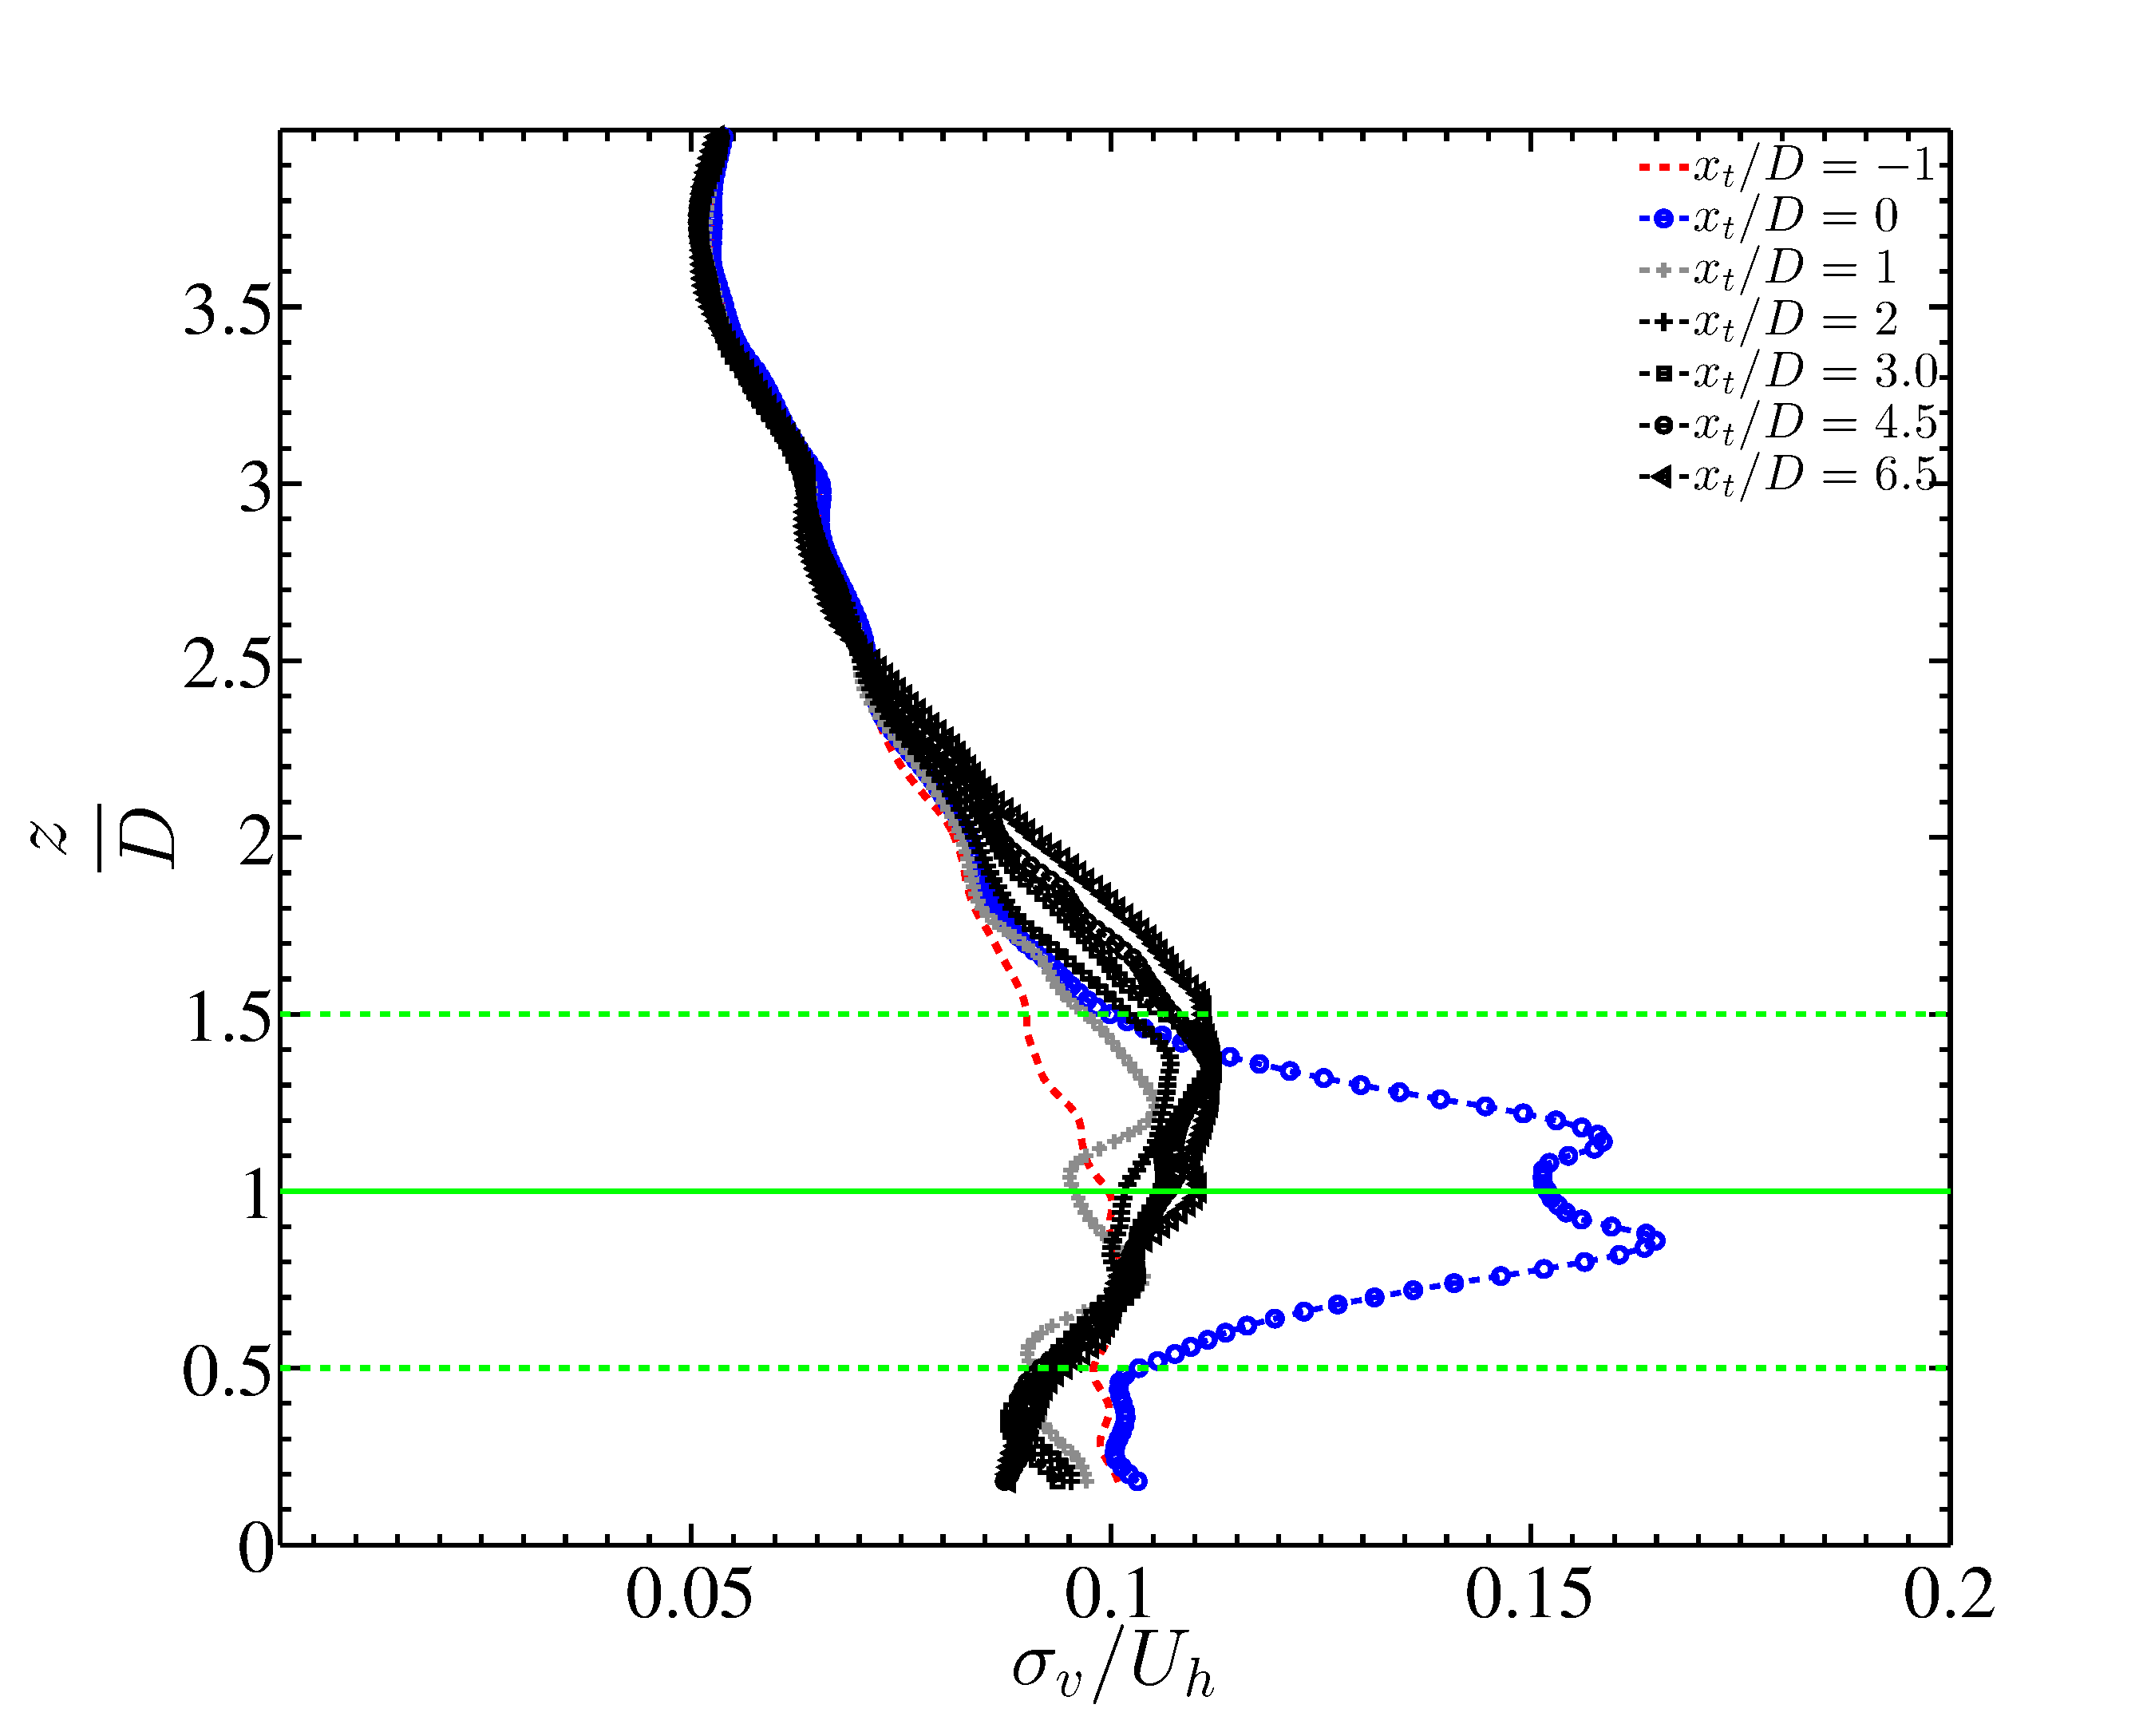
\includegraphics[width = 0.8\linewidth]{stats/vfluc_9points_avg.pdf}
\caption[Mean $\sigma_{v}$ at $x$ stations 2]{Temporally averaged mean spanwise turbulent intensity at different streamwise $x$ stations. Profile averaged over the  9 spanwise points over 3 wind turbine rotor extents.}\label{fig:vstat2}
\end{figure}
\begin{figure}
\centering
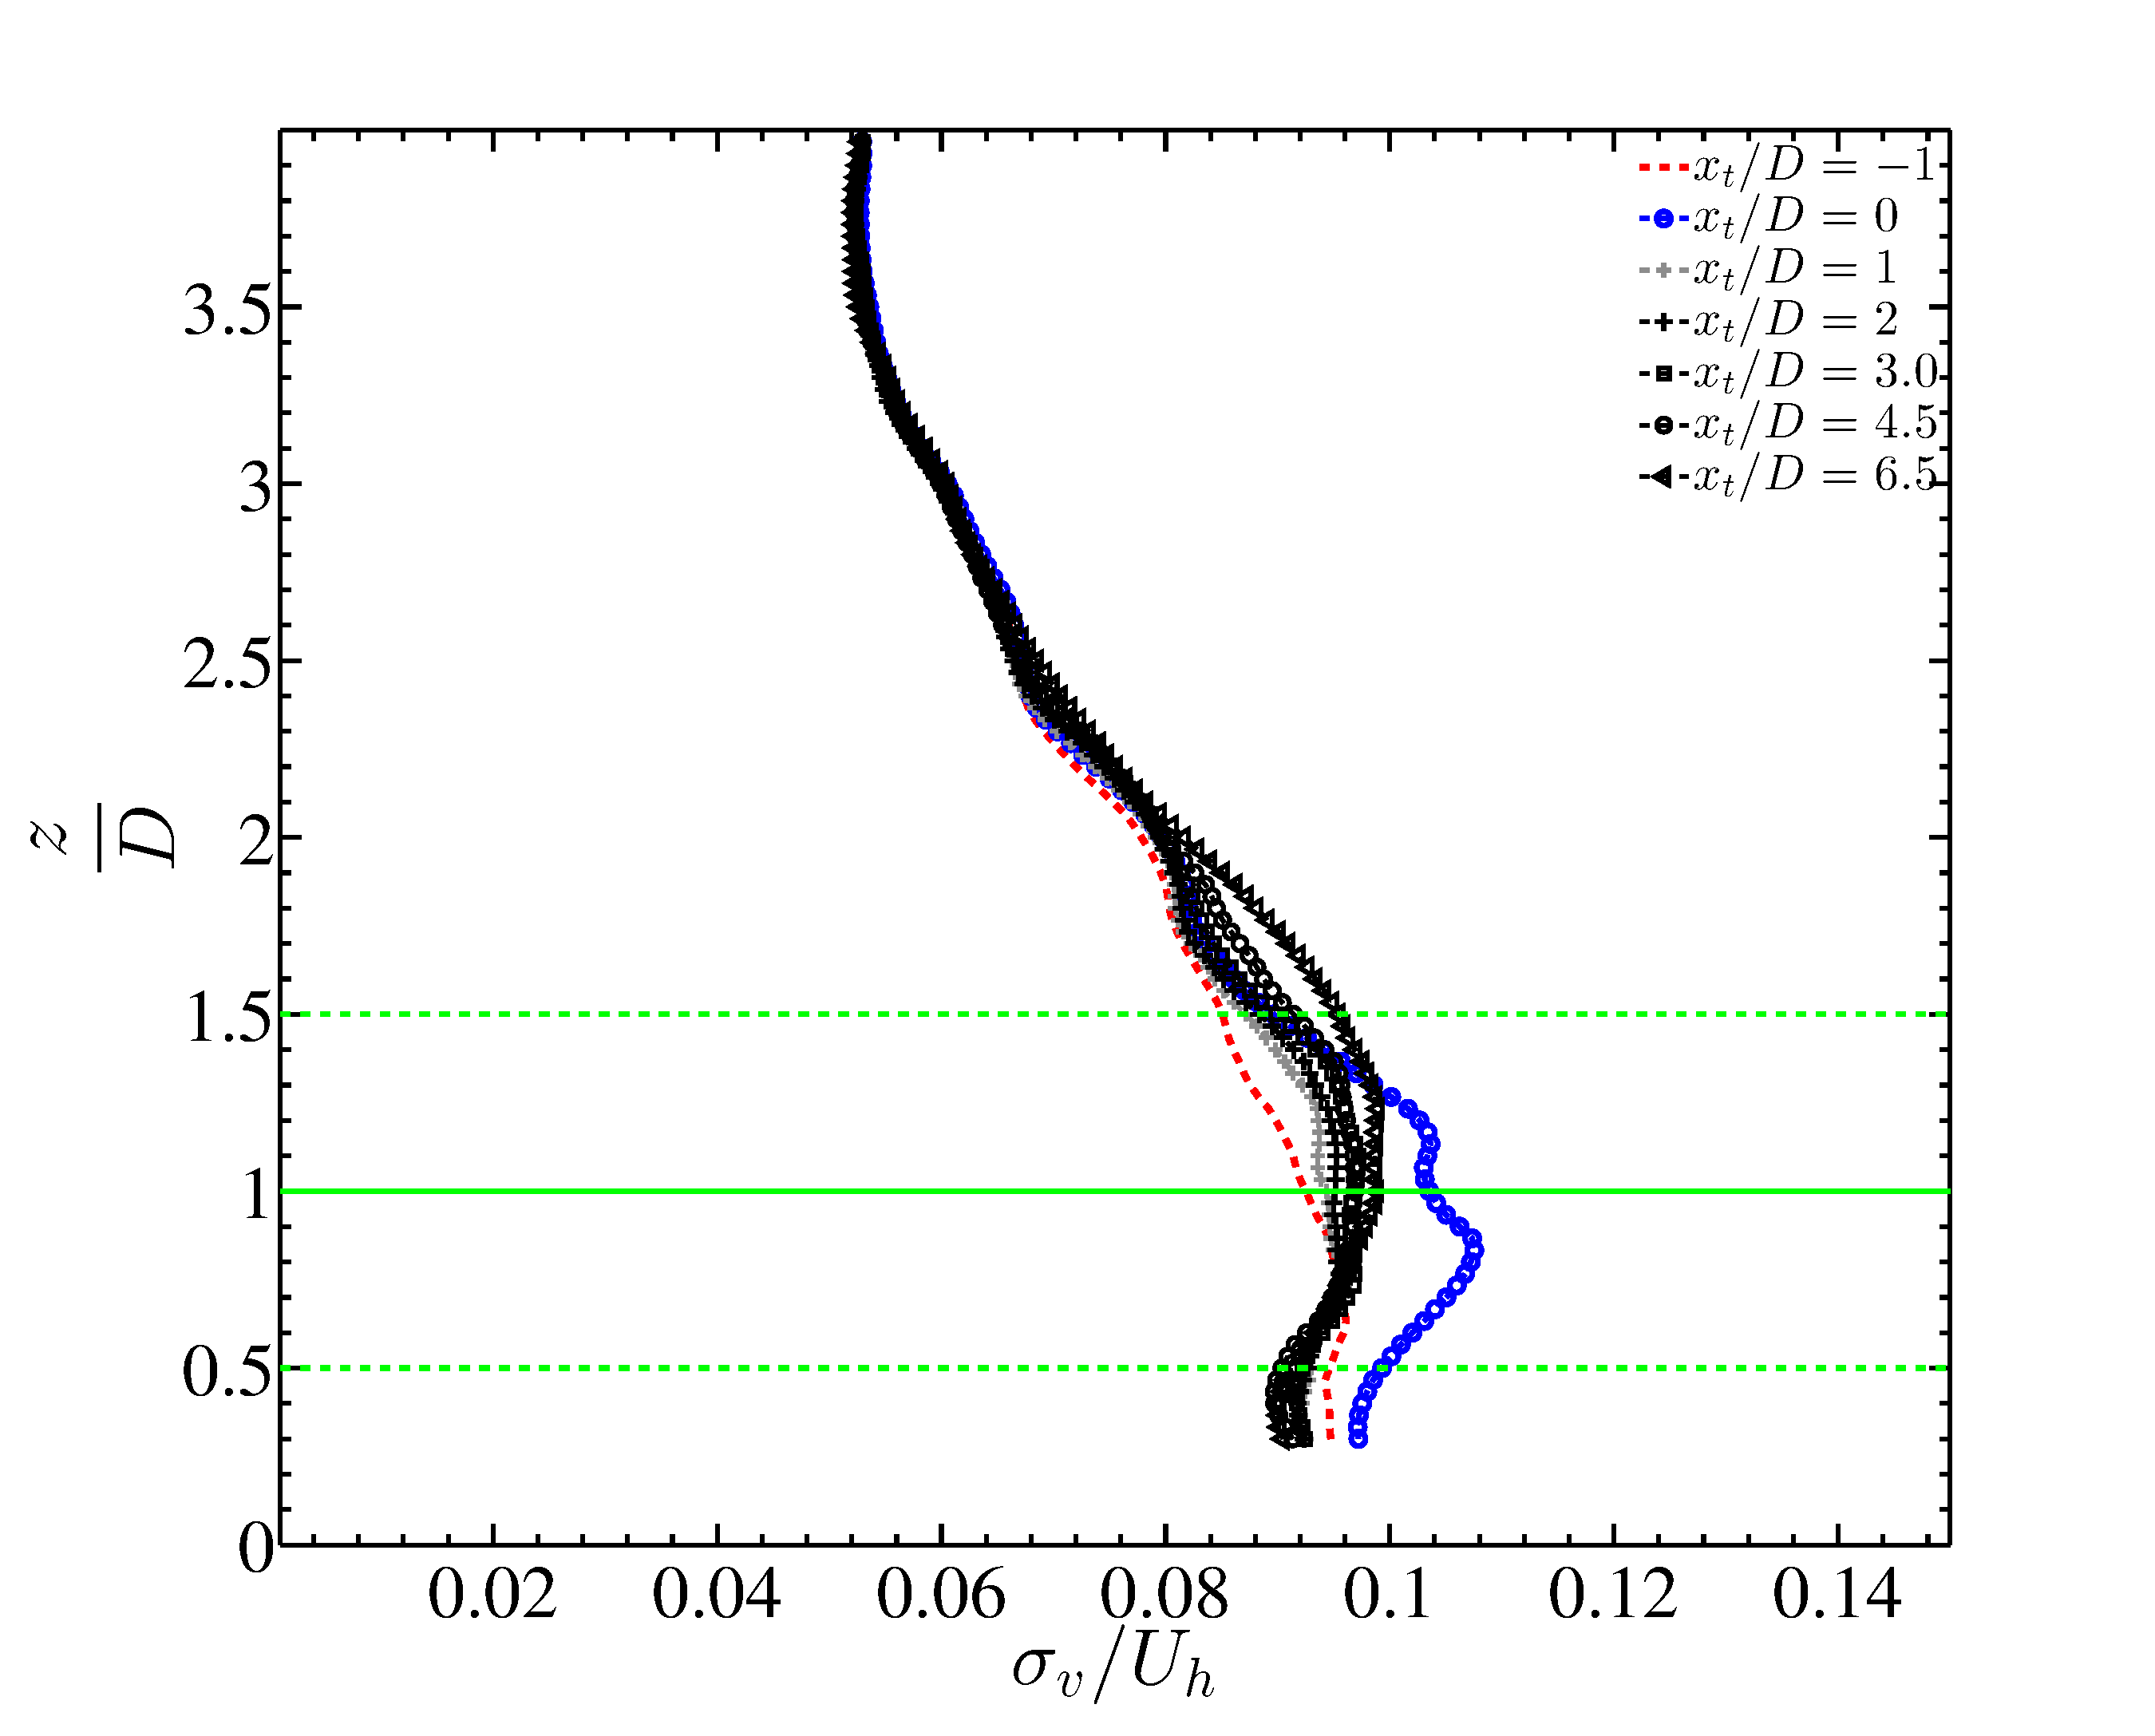
\includegraphics[width = 0.8\linewidth]{stats/vfluc_Npoints_avg.pdf}
\caption[Mean $\sigma_{v}$ at $x$ stations 3]{Temporally averaged mean spanwise turbulent intensity at different streamwise $x$ stations. Profile averaged over the whole spanwise domain.}\label{fig:vstat3}
\end{figure}
%--------------------------------------------------------------------------------------%
\begin{figure}
\centering
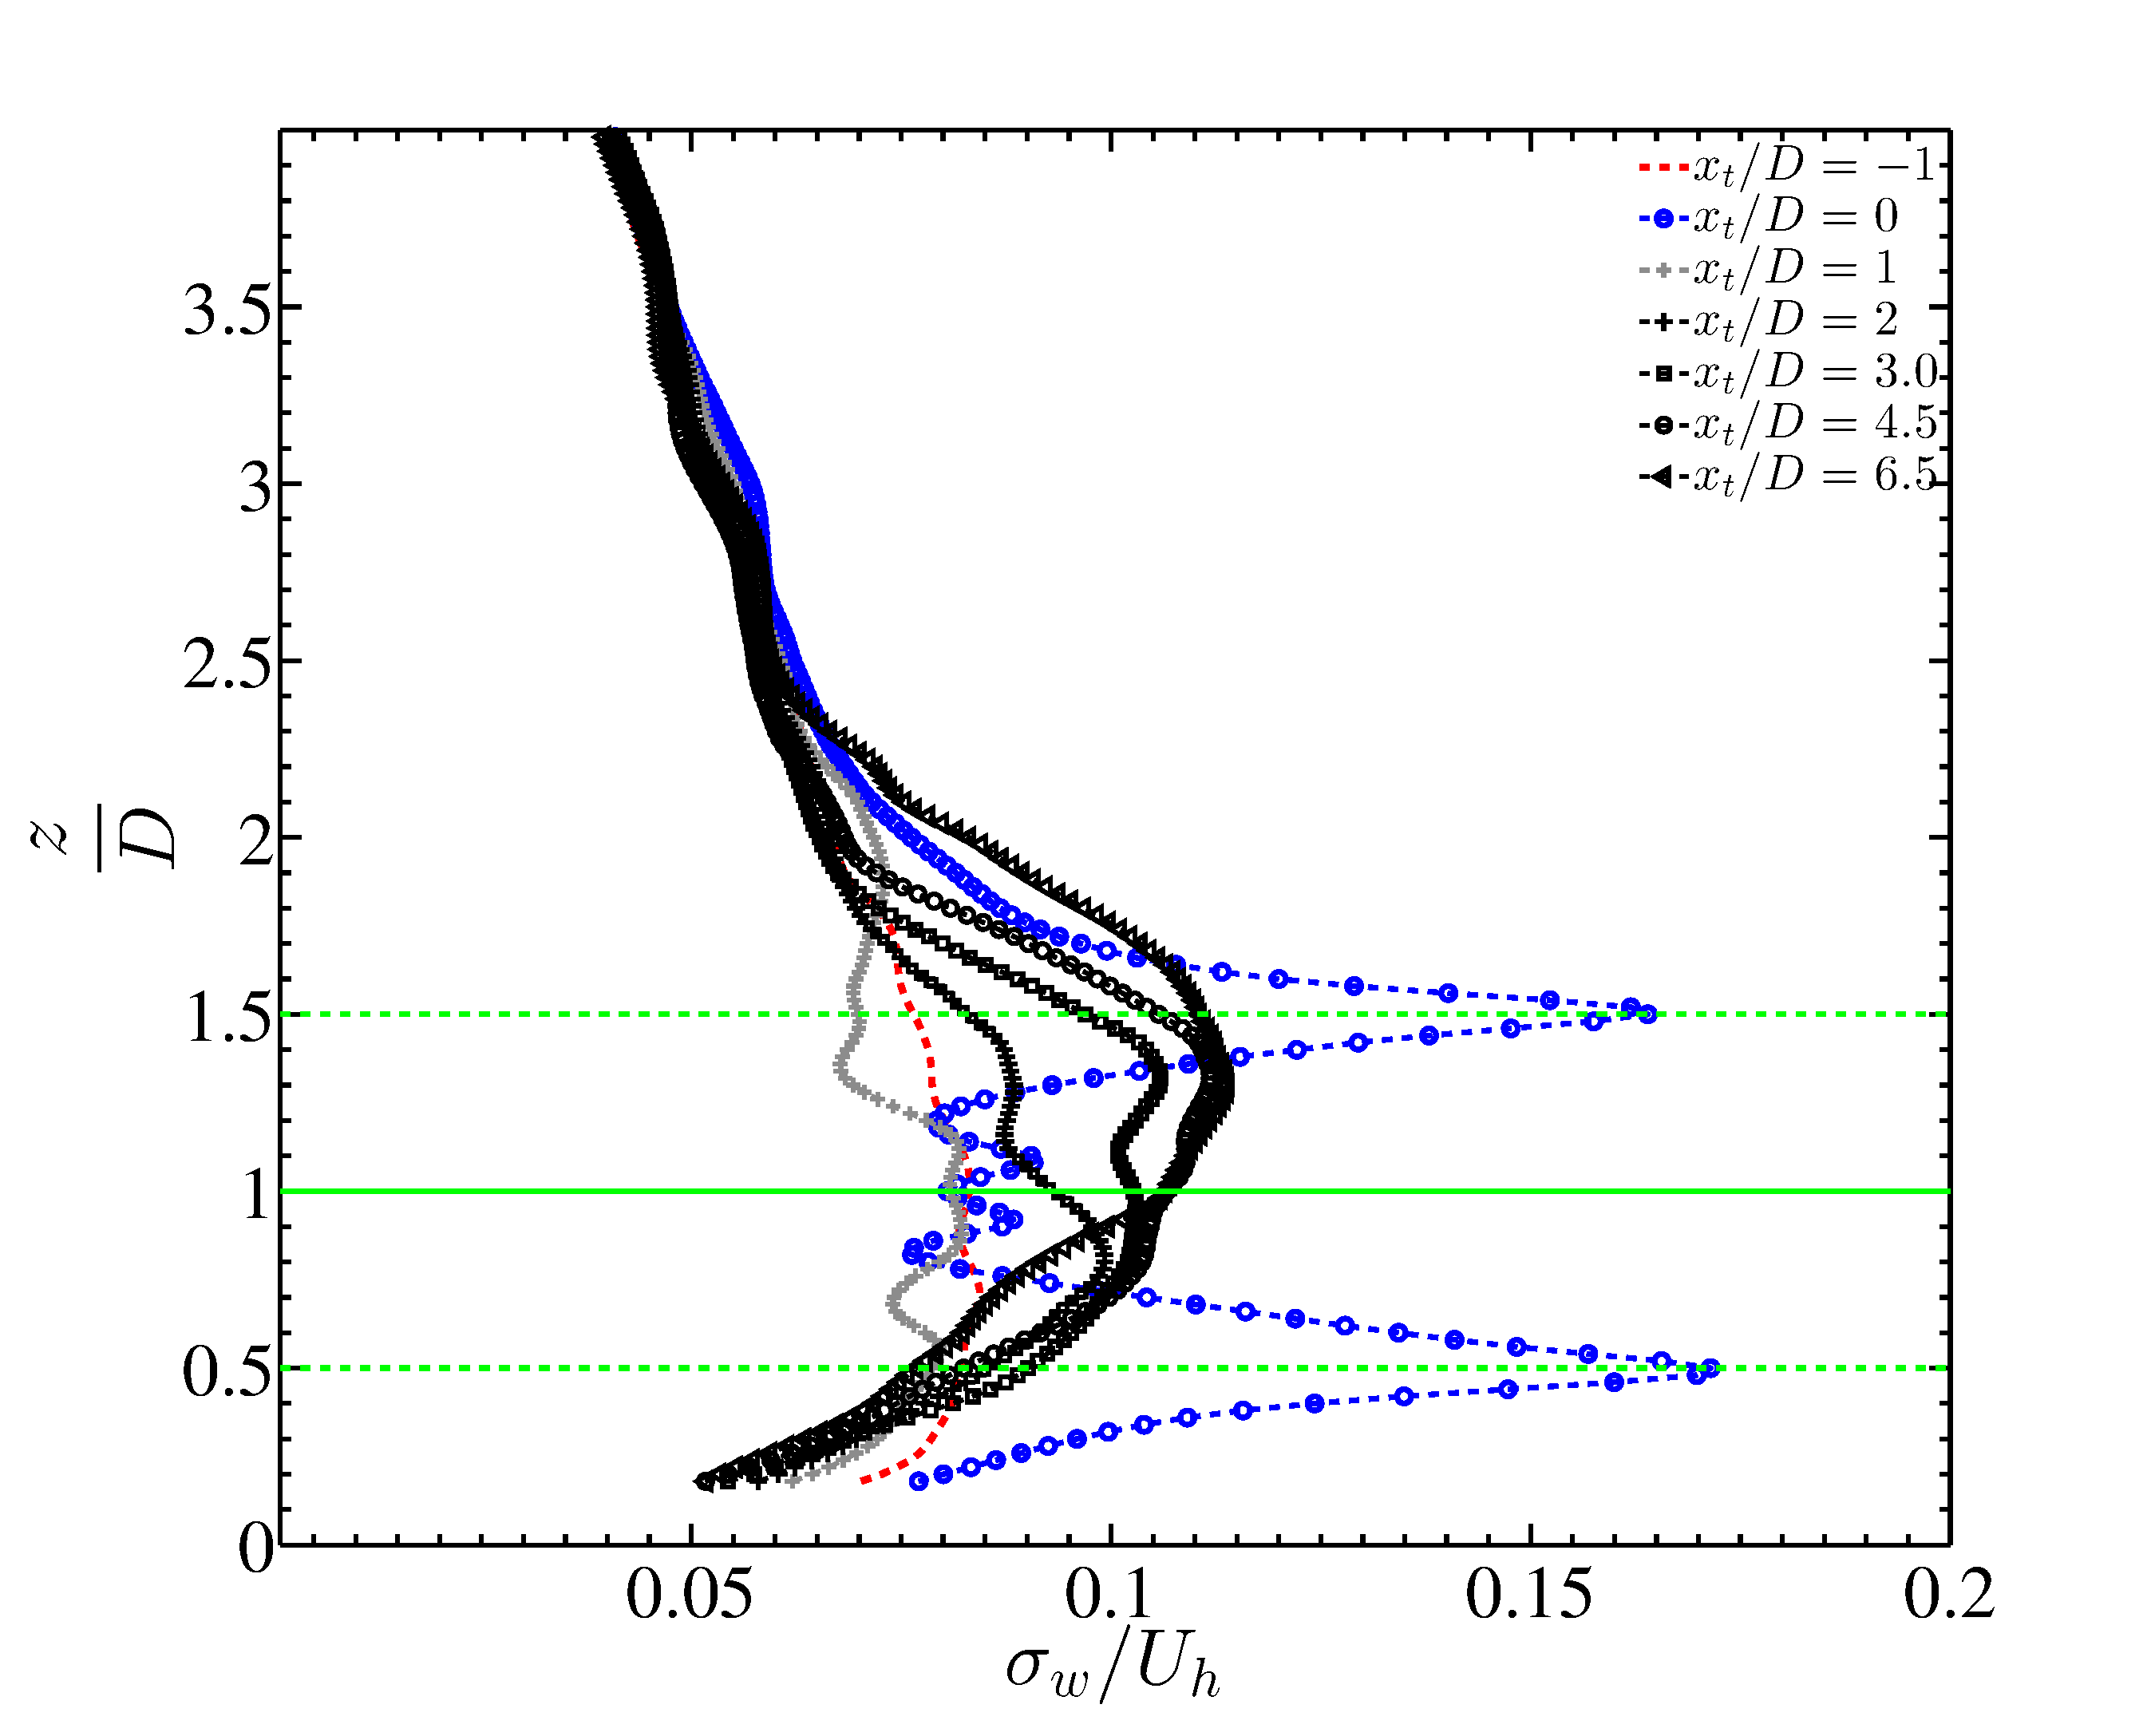
\includegraphics[width = 0.8\linewidth]{stats/wfluc_3points_avg.pdf}
\caption[Mean $\sigma_{w}$ at $x$ stations 1]{Temporally averaged wall normal turbulent intensity at different streamwise $x$ stations. Profile averaged over the  3 spanwise points (center of turbine rotor).}\label{fig:wstat1}
\end{figure}
\begin{figure}
\centering
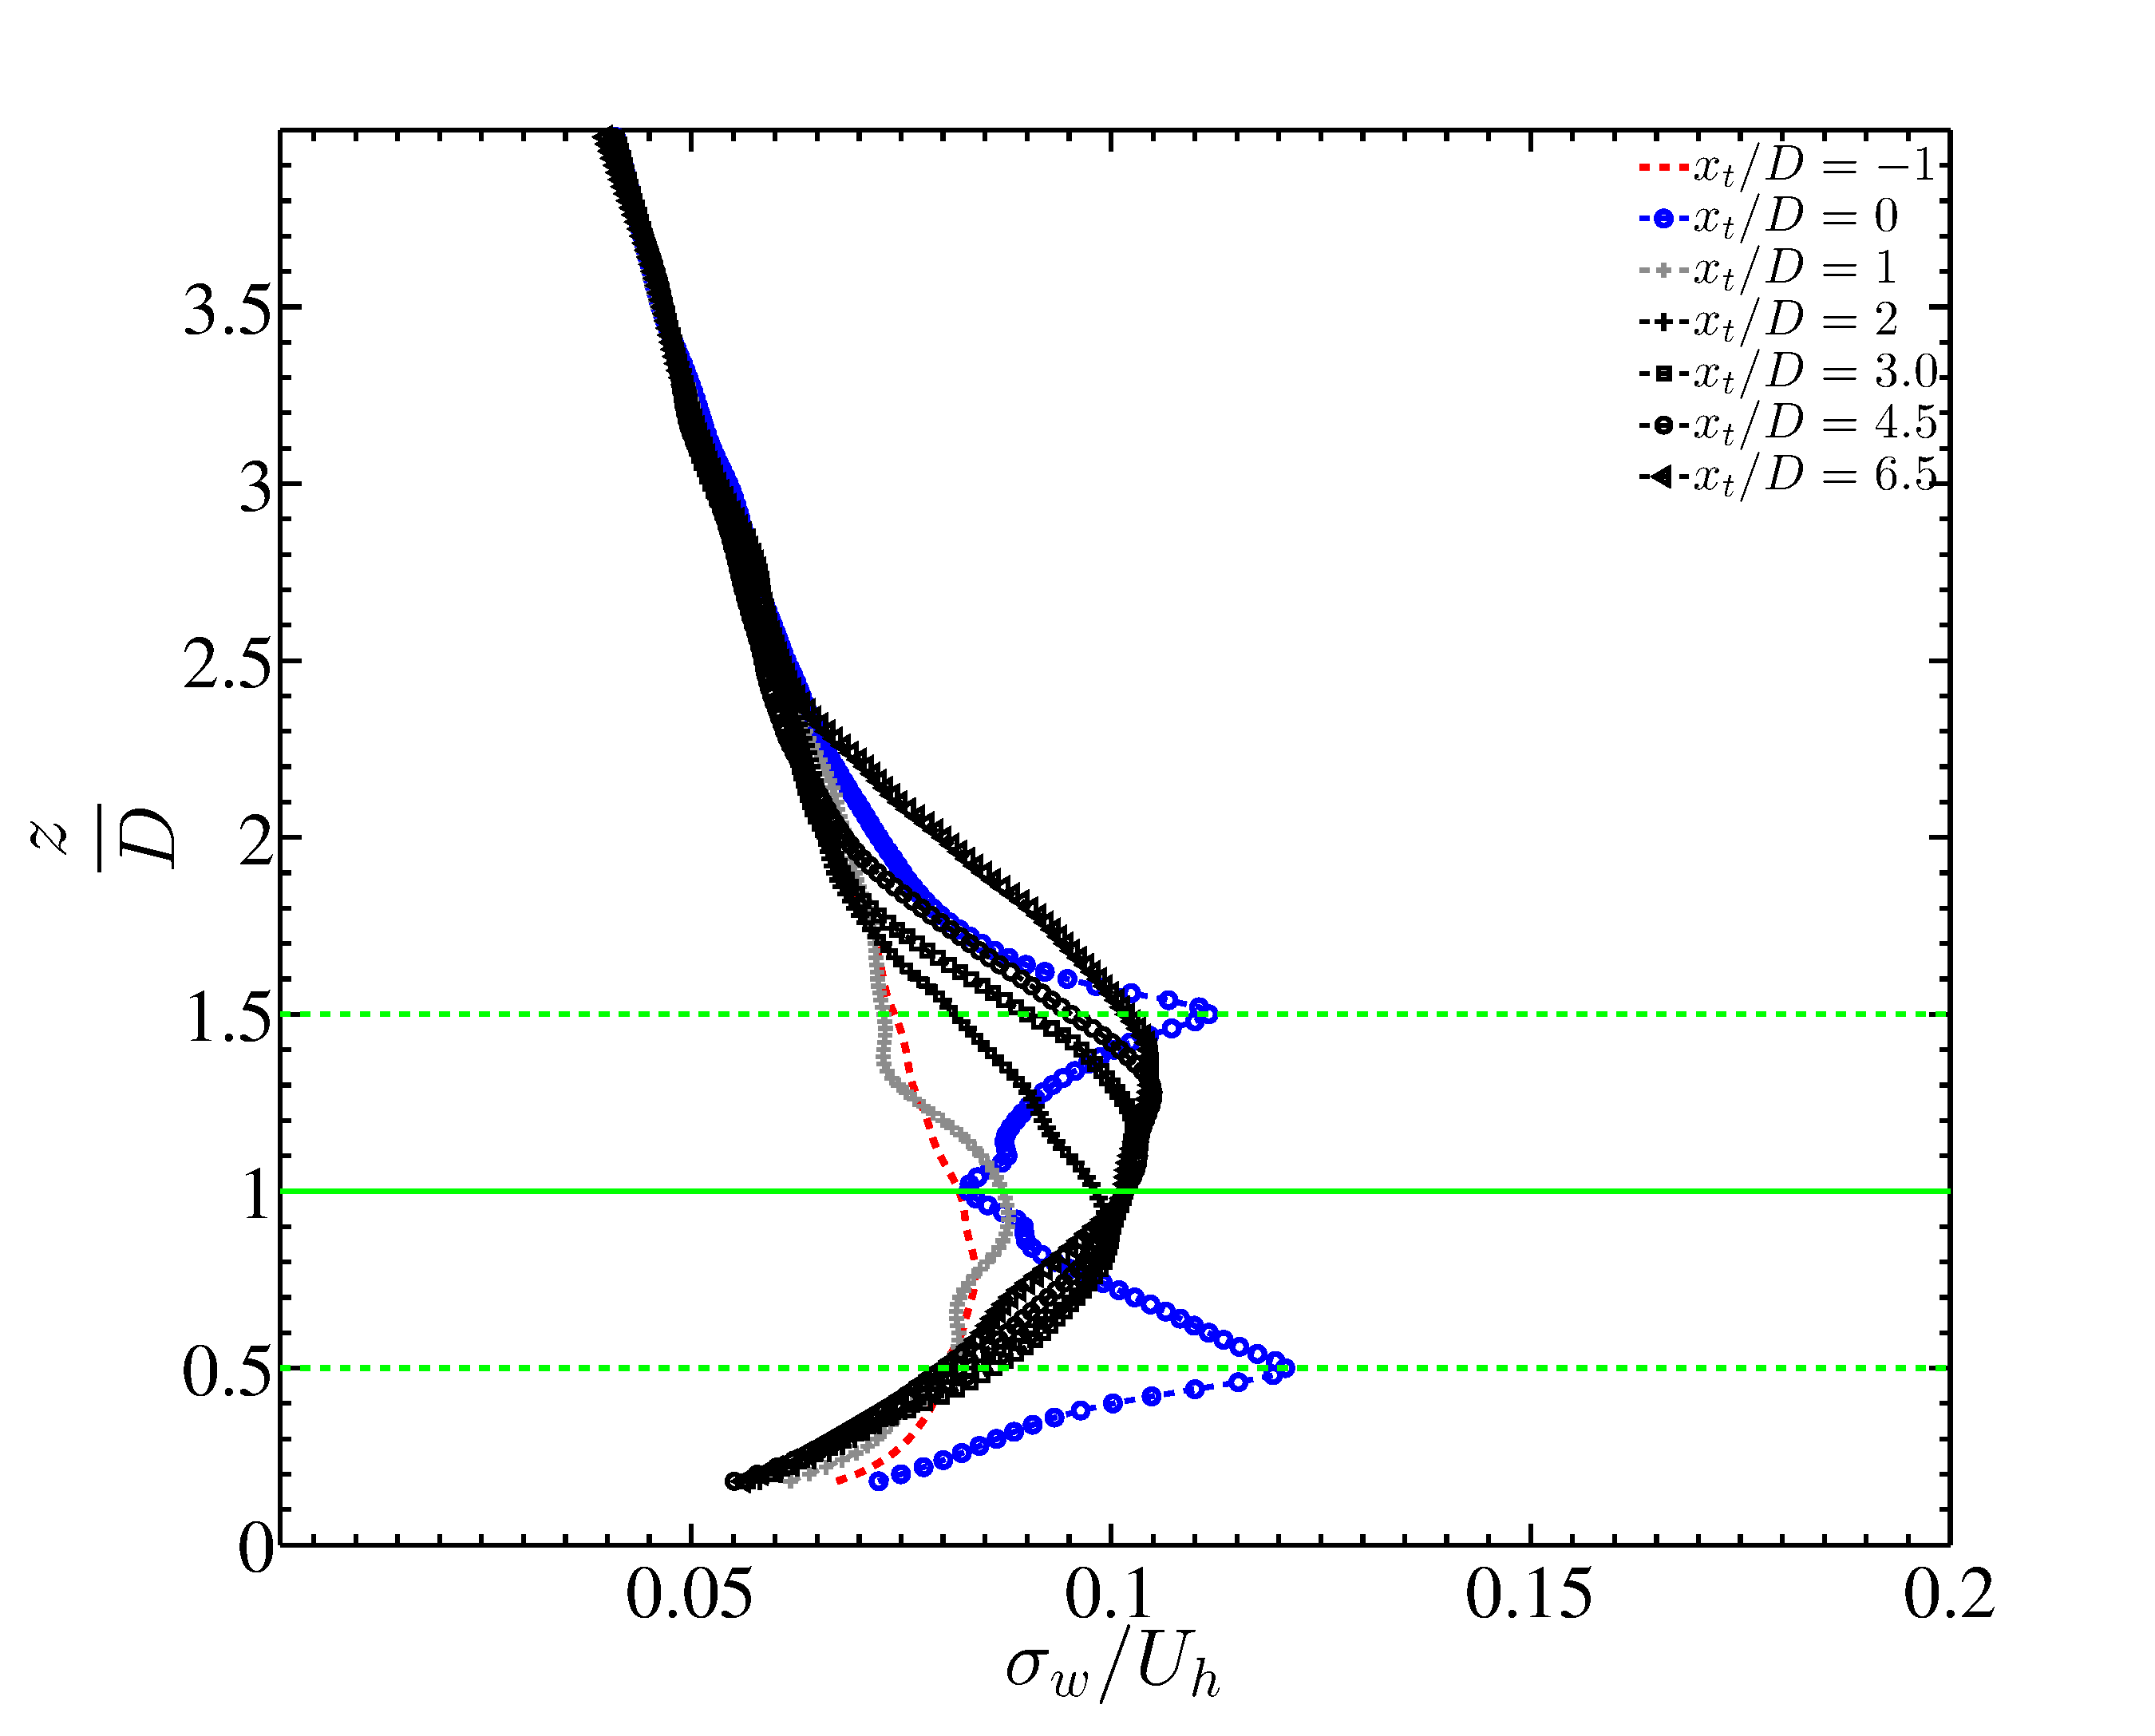
\includegraphics[width = 0.8\linewidth]{stats/wfluc_9points_avg.pdf}
\caption[Mean $\sigma_{w}$ at $x$ stations 2]{Temporally averaged mean wall normal turbulent intensity at different streamwise $x$ stations. Profile averaged over the  9 spanwise points over 3 wind turbine rotor extents.}\label{fig:wstat2}
\end{figure}
\begin{figure}
\centering
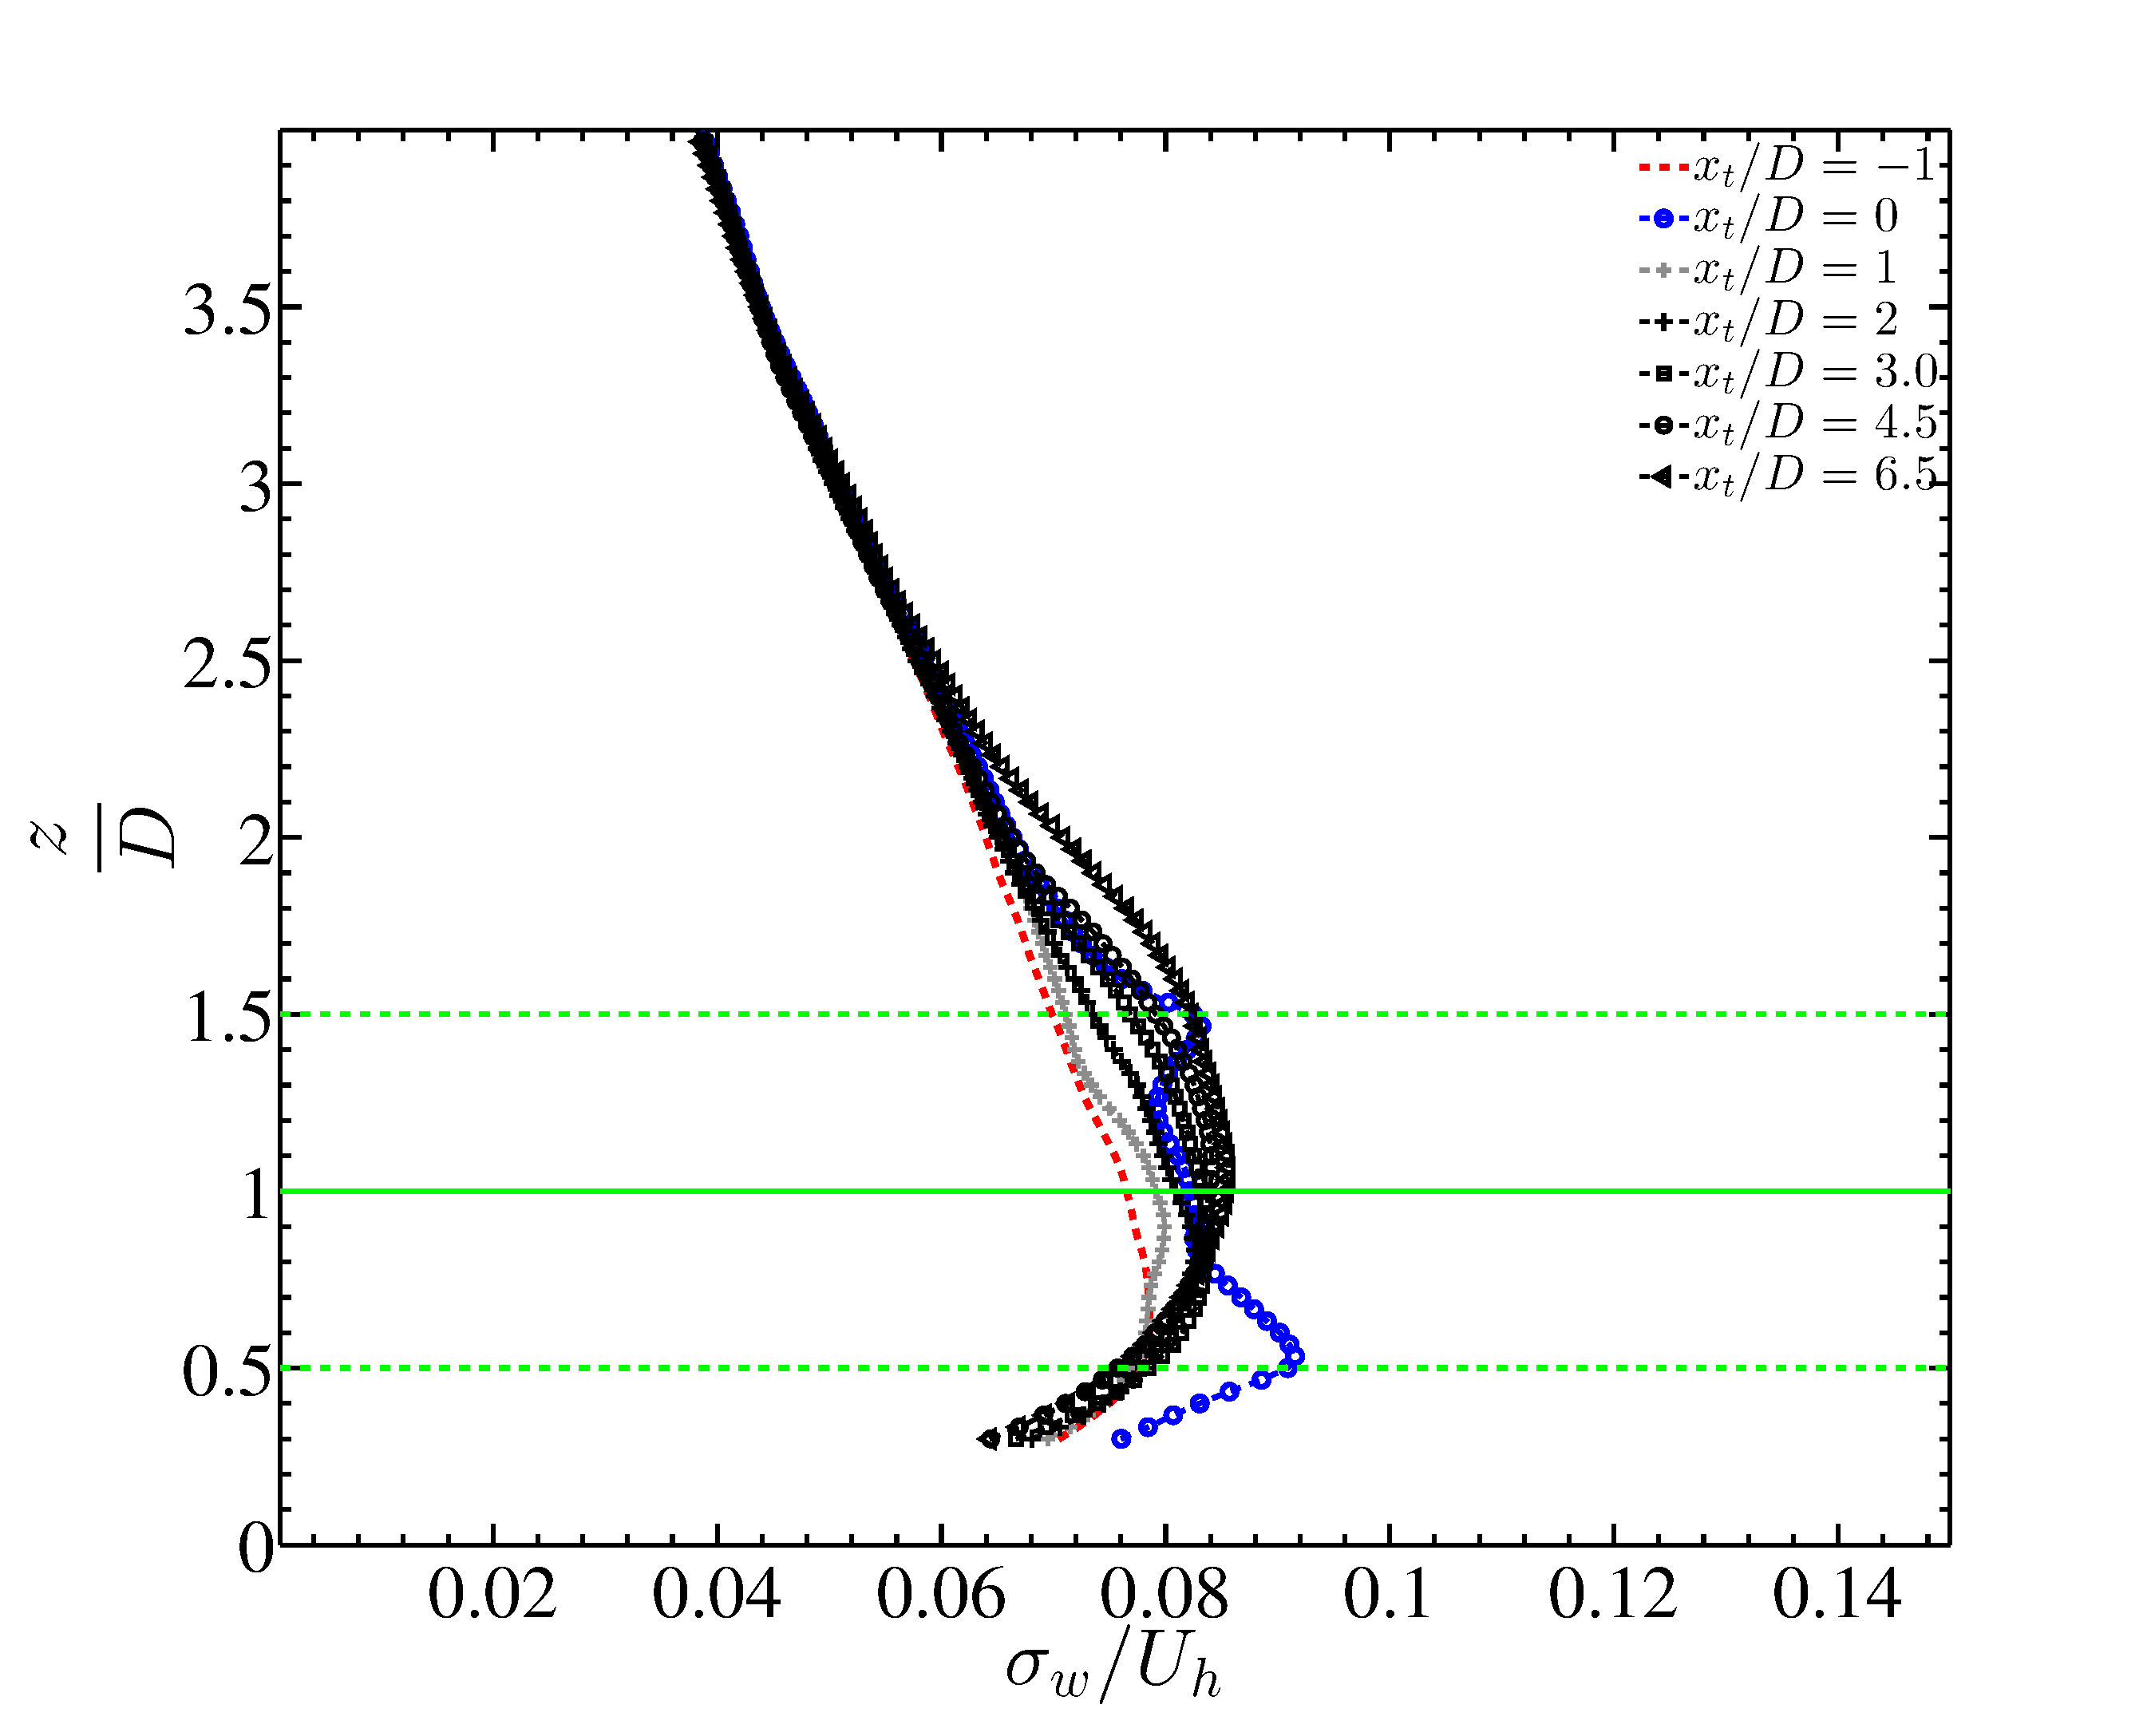
\includegraphics[width = 0.8\linewidth]{stats/wfluc_Npoints_avg.pdf}
\caption[Mean $\sigma_{w}$ at $x$ stations 3]{Temporally averaged mean wall normal turbulent intensity at different streamwise $x$ stations. Profile averaged over the whole spanwise domain.}\label{fig:wstat3}
\end{figure}




\begin{figure}
\centering
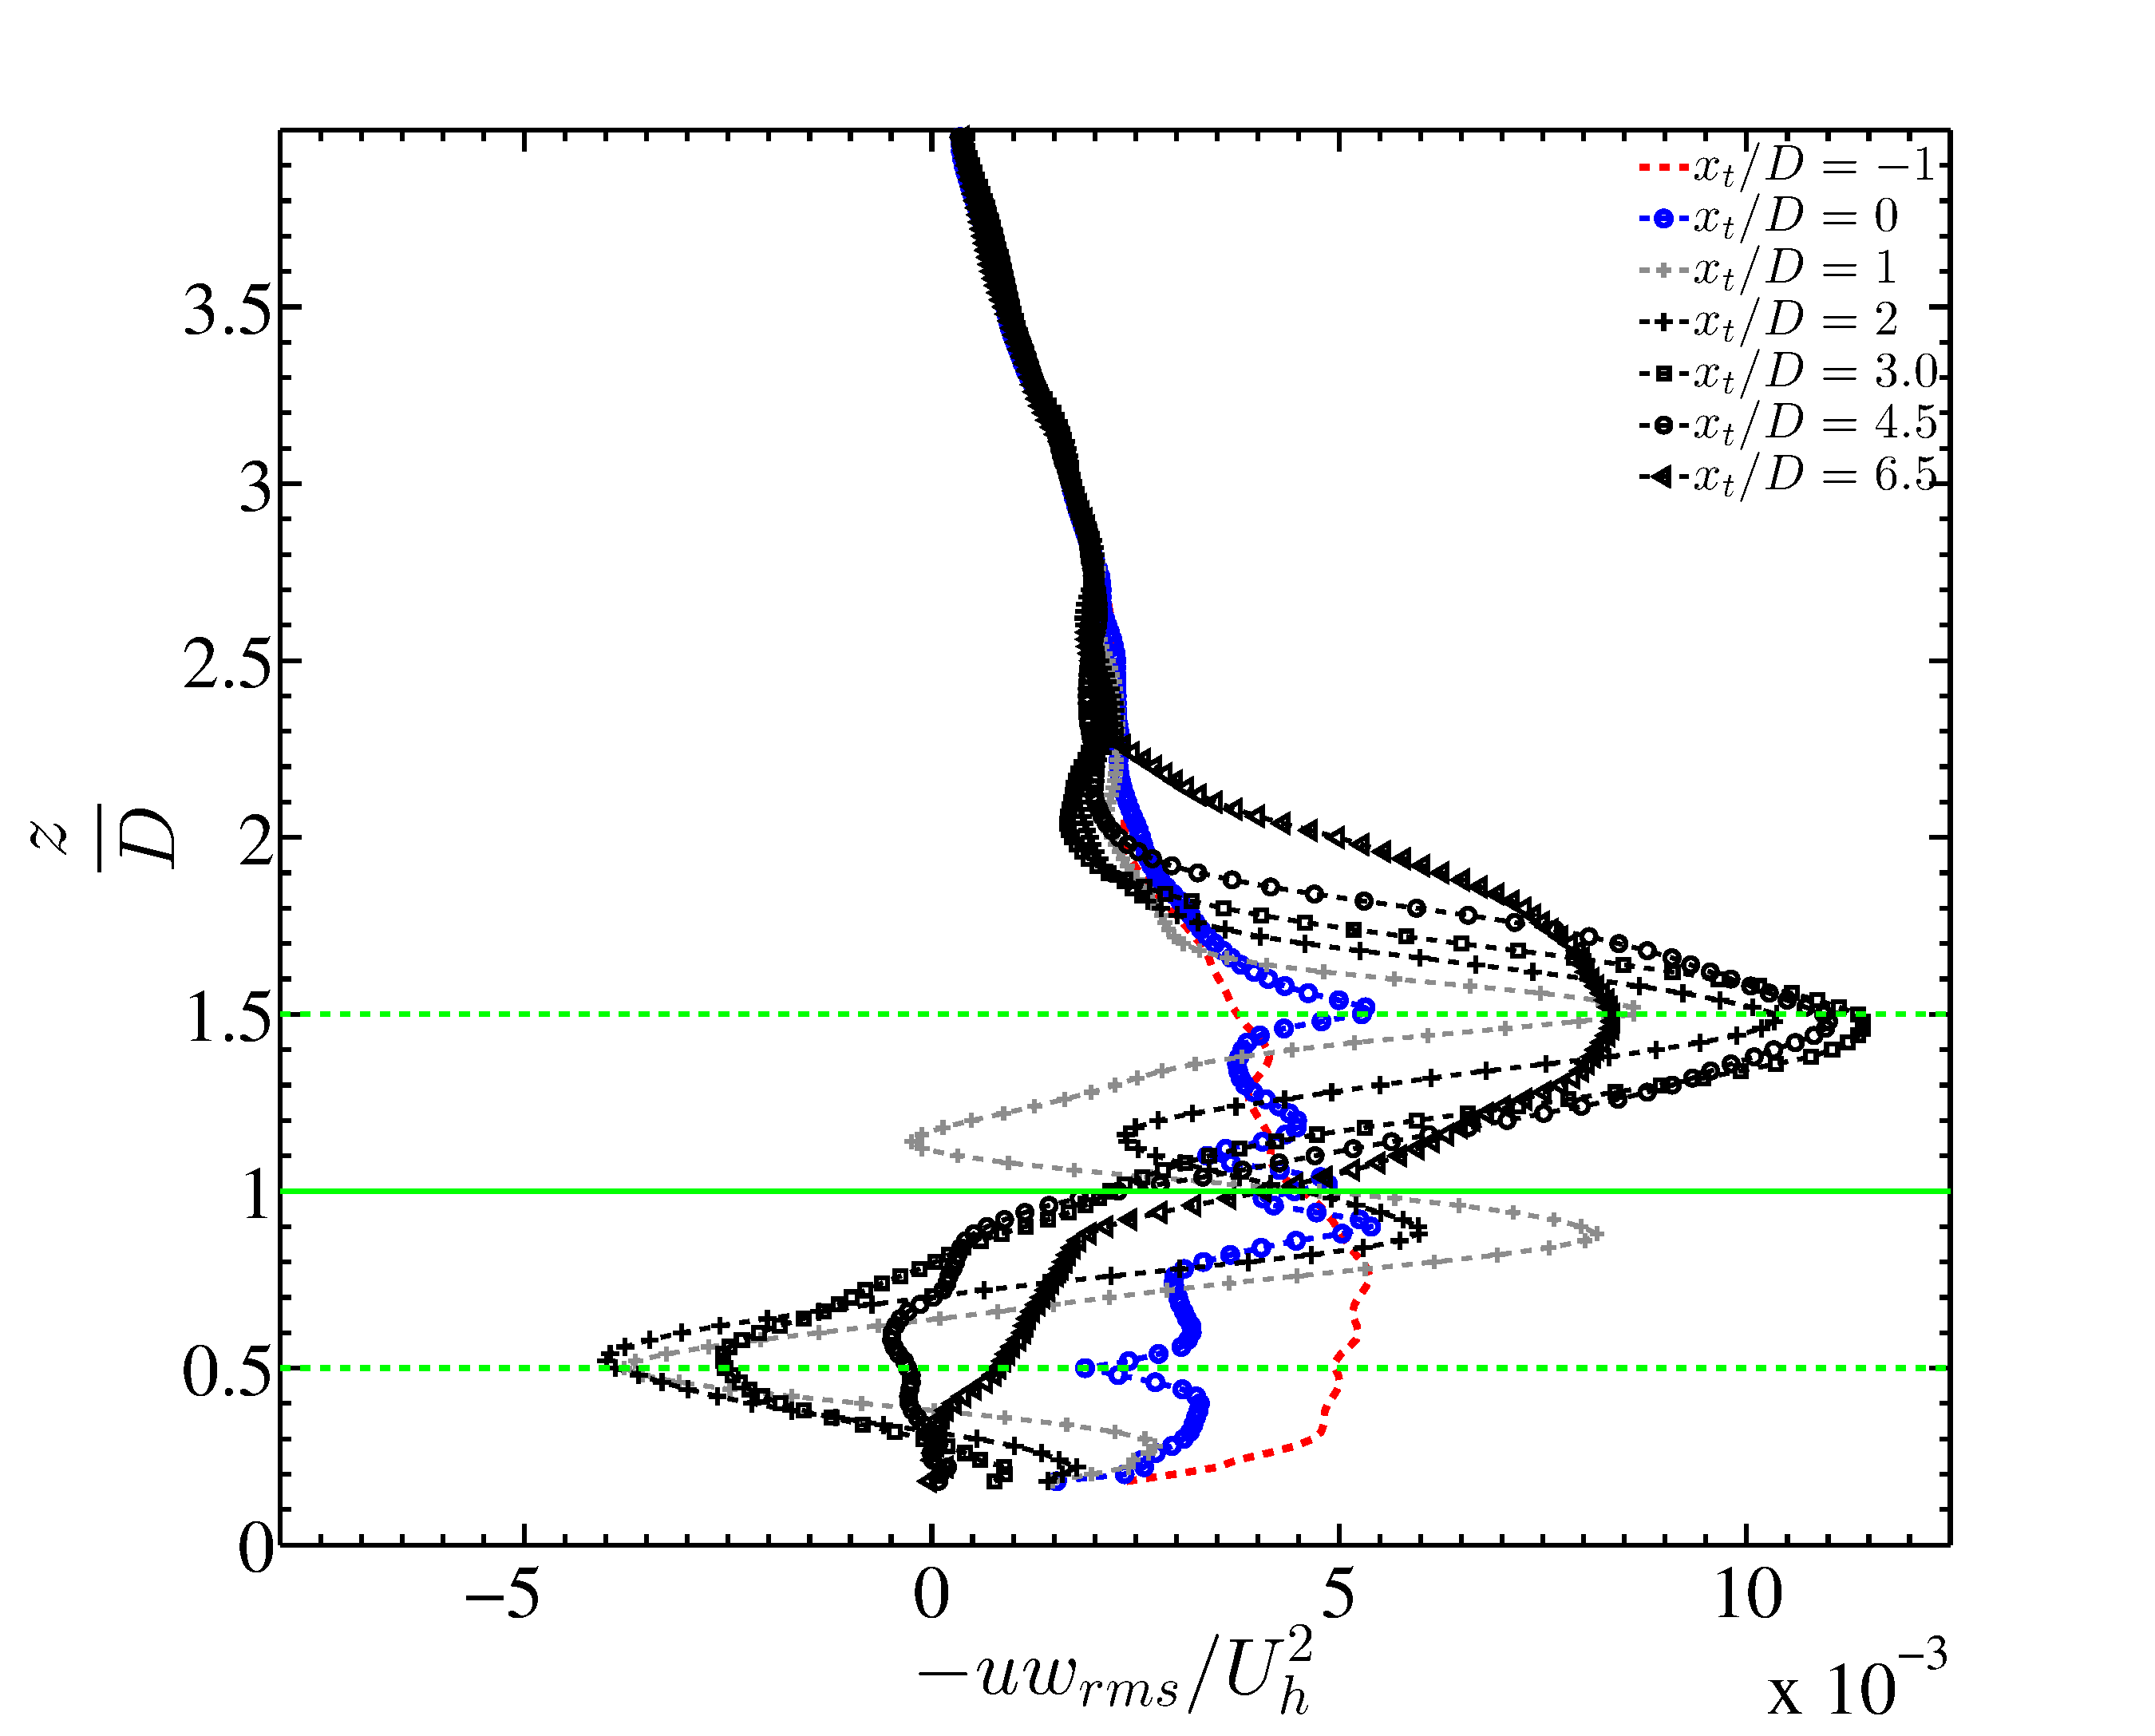
\includegraphics[width = 0.8\linewidth]{stats/shrprof_3points_avg.pdf}
\caption[Mean shear stress at $x$ stations 1]{Temporally averaged mean turbulent kinematic shear stress at different streamwise $x$ stations. Profile averaged over the  3 spanwise points (center of turbine rotor).}\label{fig:shrstat1}
\end{figure}
\begin{figure}
\centering
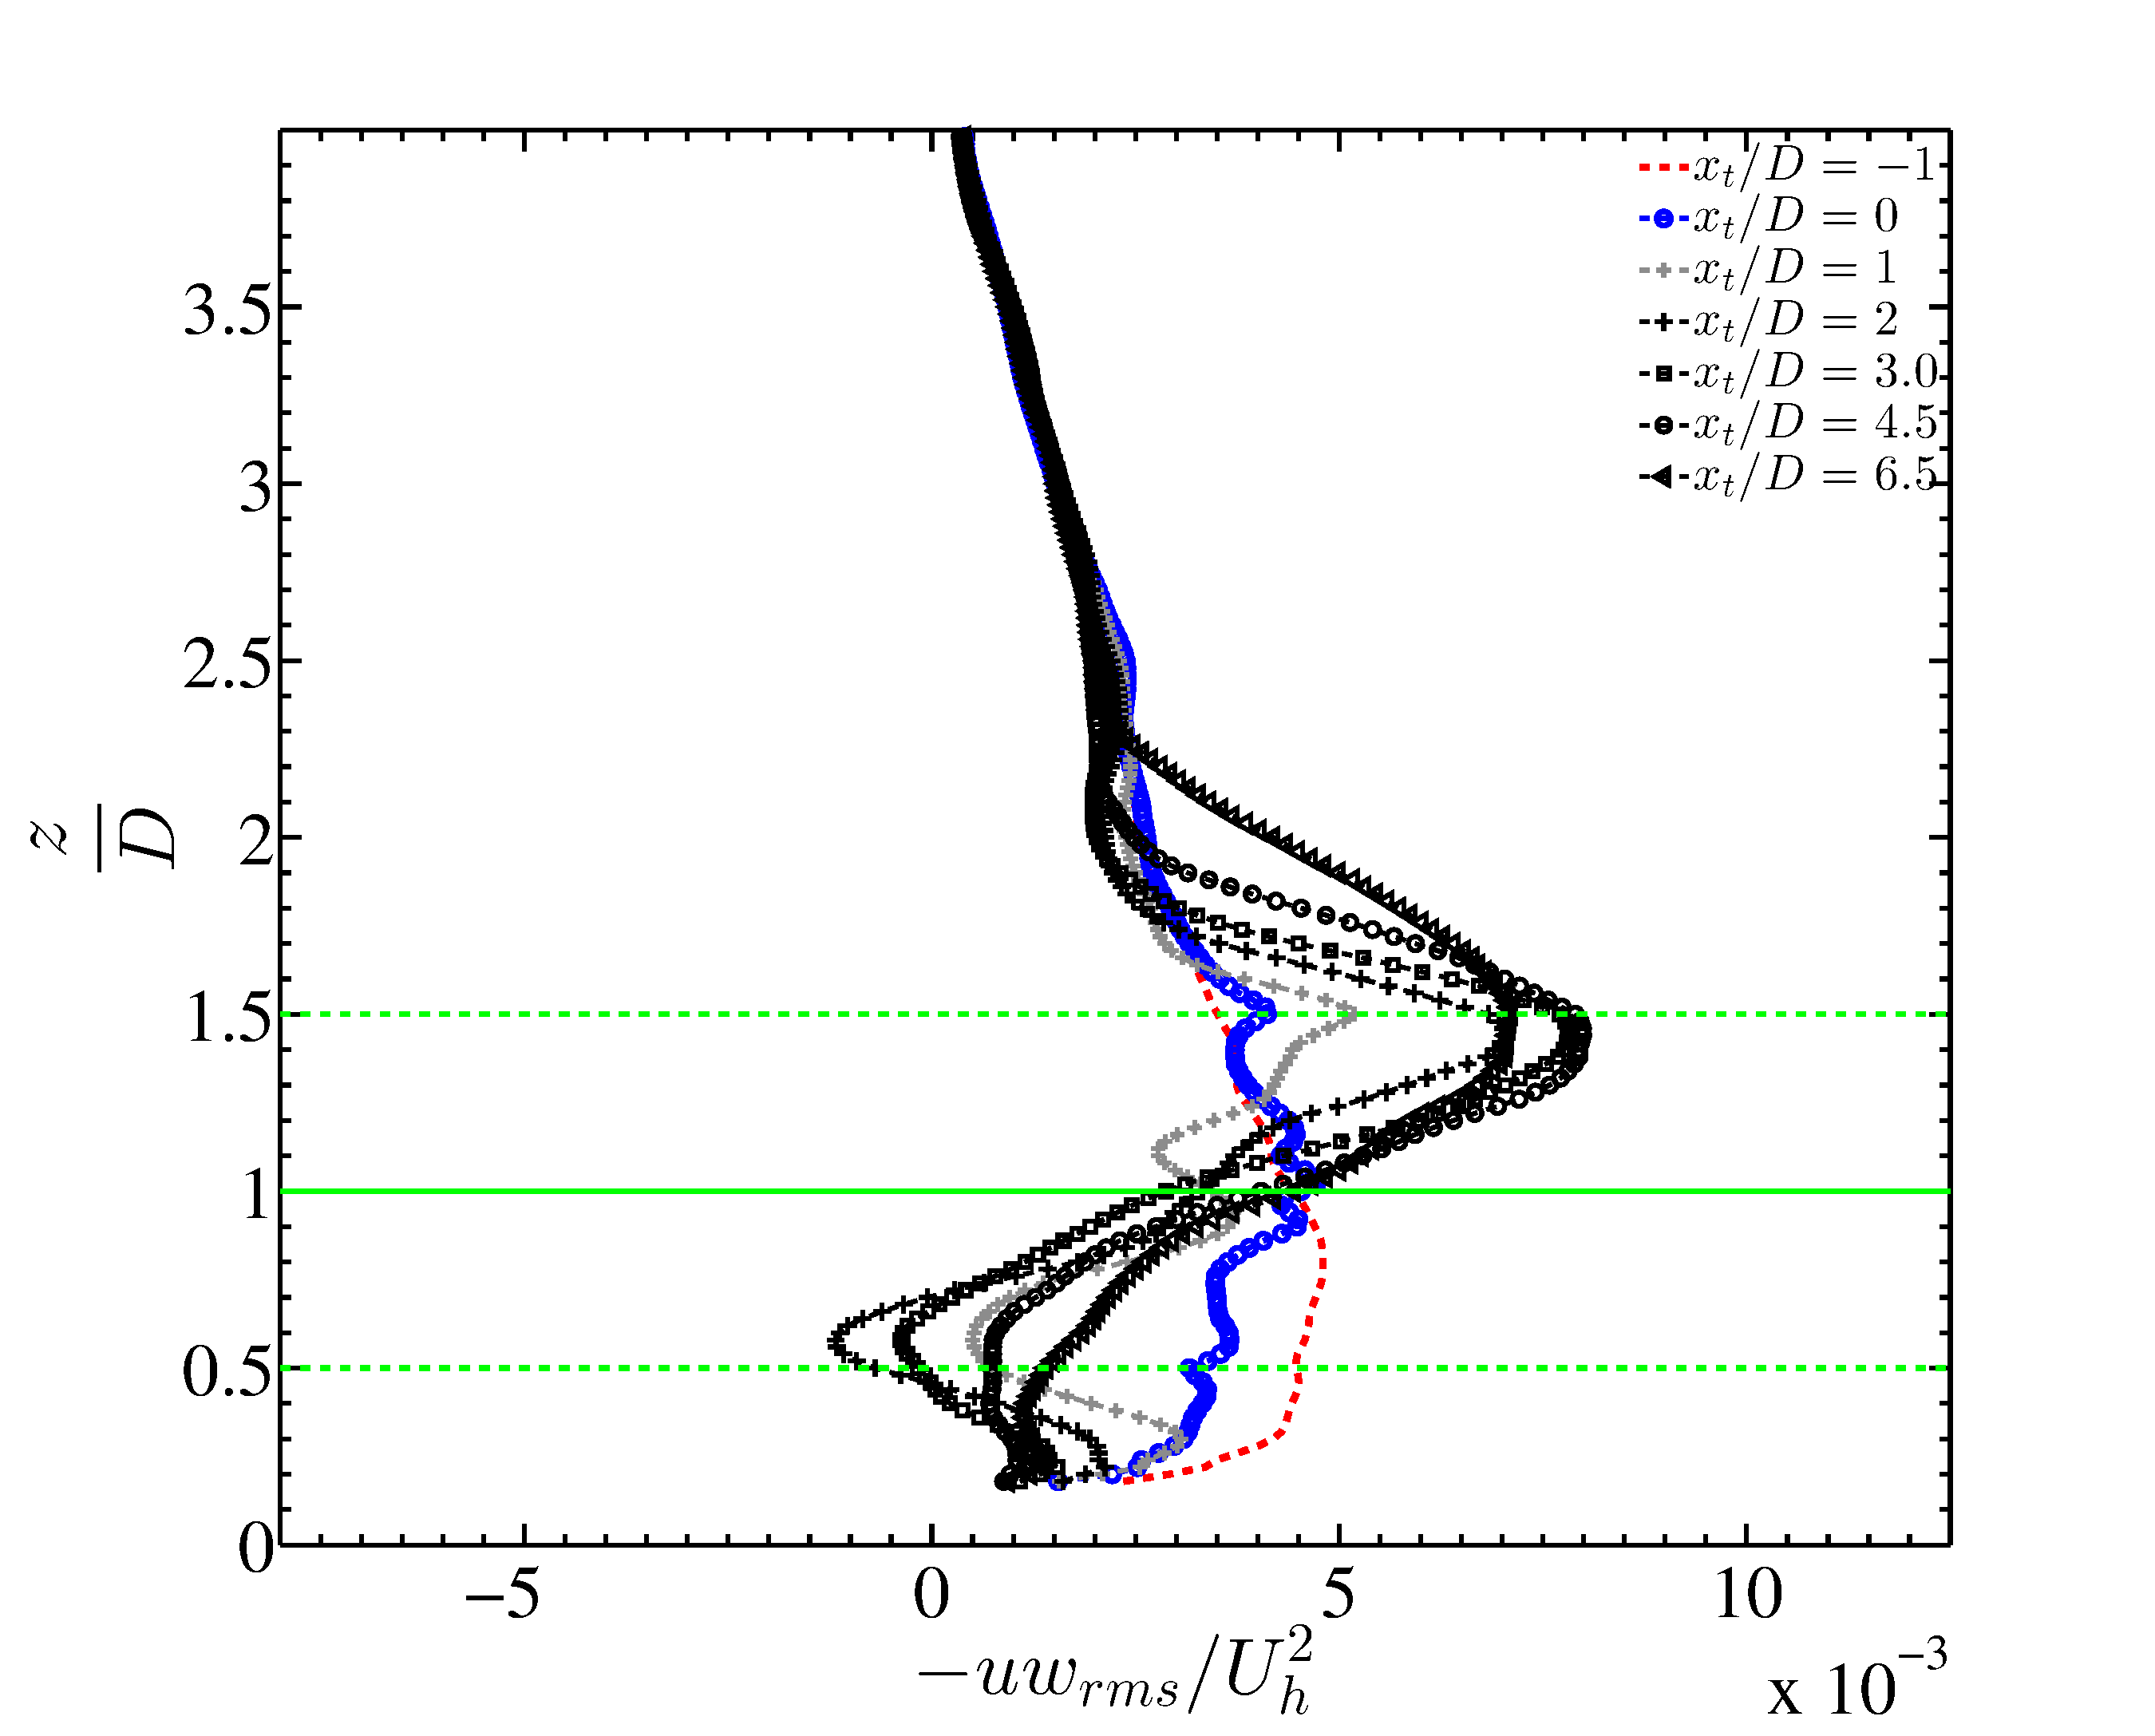
\includegraphics[width = 0.8\linewidth]{stats/shrprof_9points_avg.pdf}
\caption[Mean shear stress at $x$ stations 2]{Temporally averaged mean turbulent kinematic shear stress at different streamwise $x$ stations. Profile averaged over the  9 spanwise points over 3 wind turbine rotor extents.}\label{fig:shrstat2}
\end{figure}
\begin{figure}
\centering
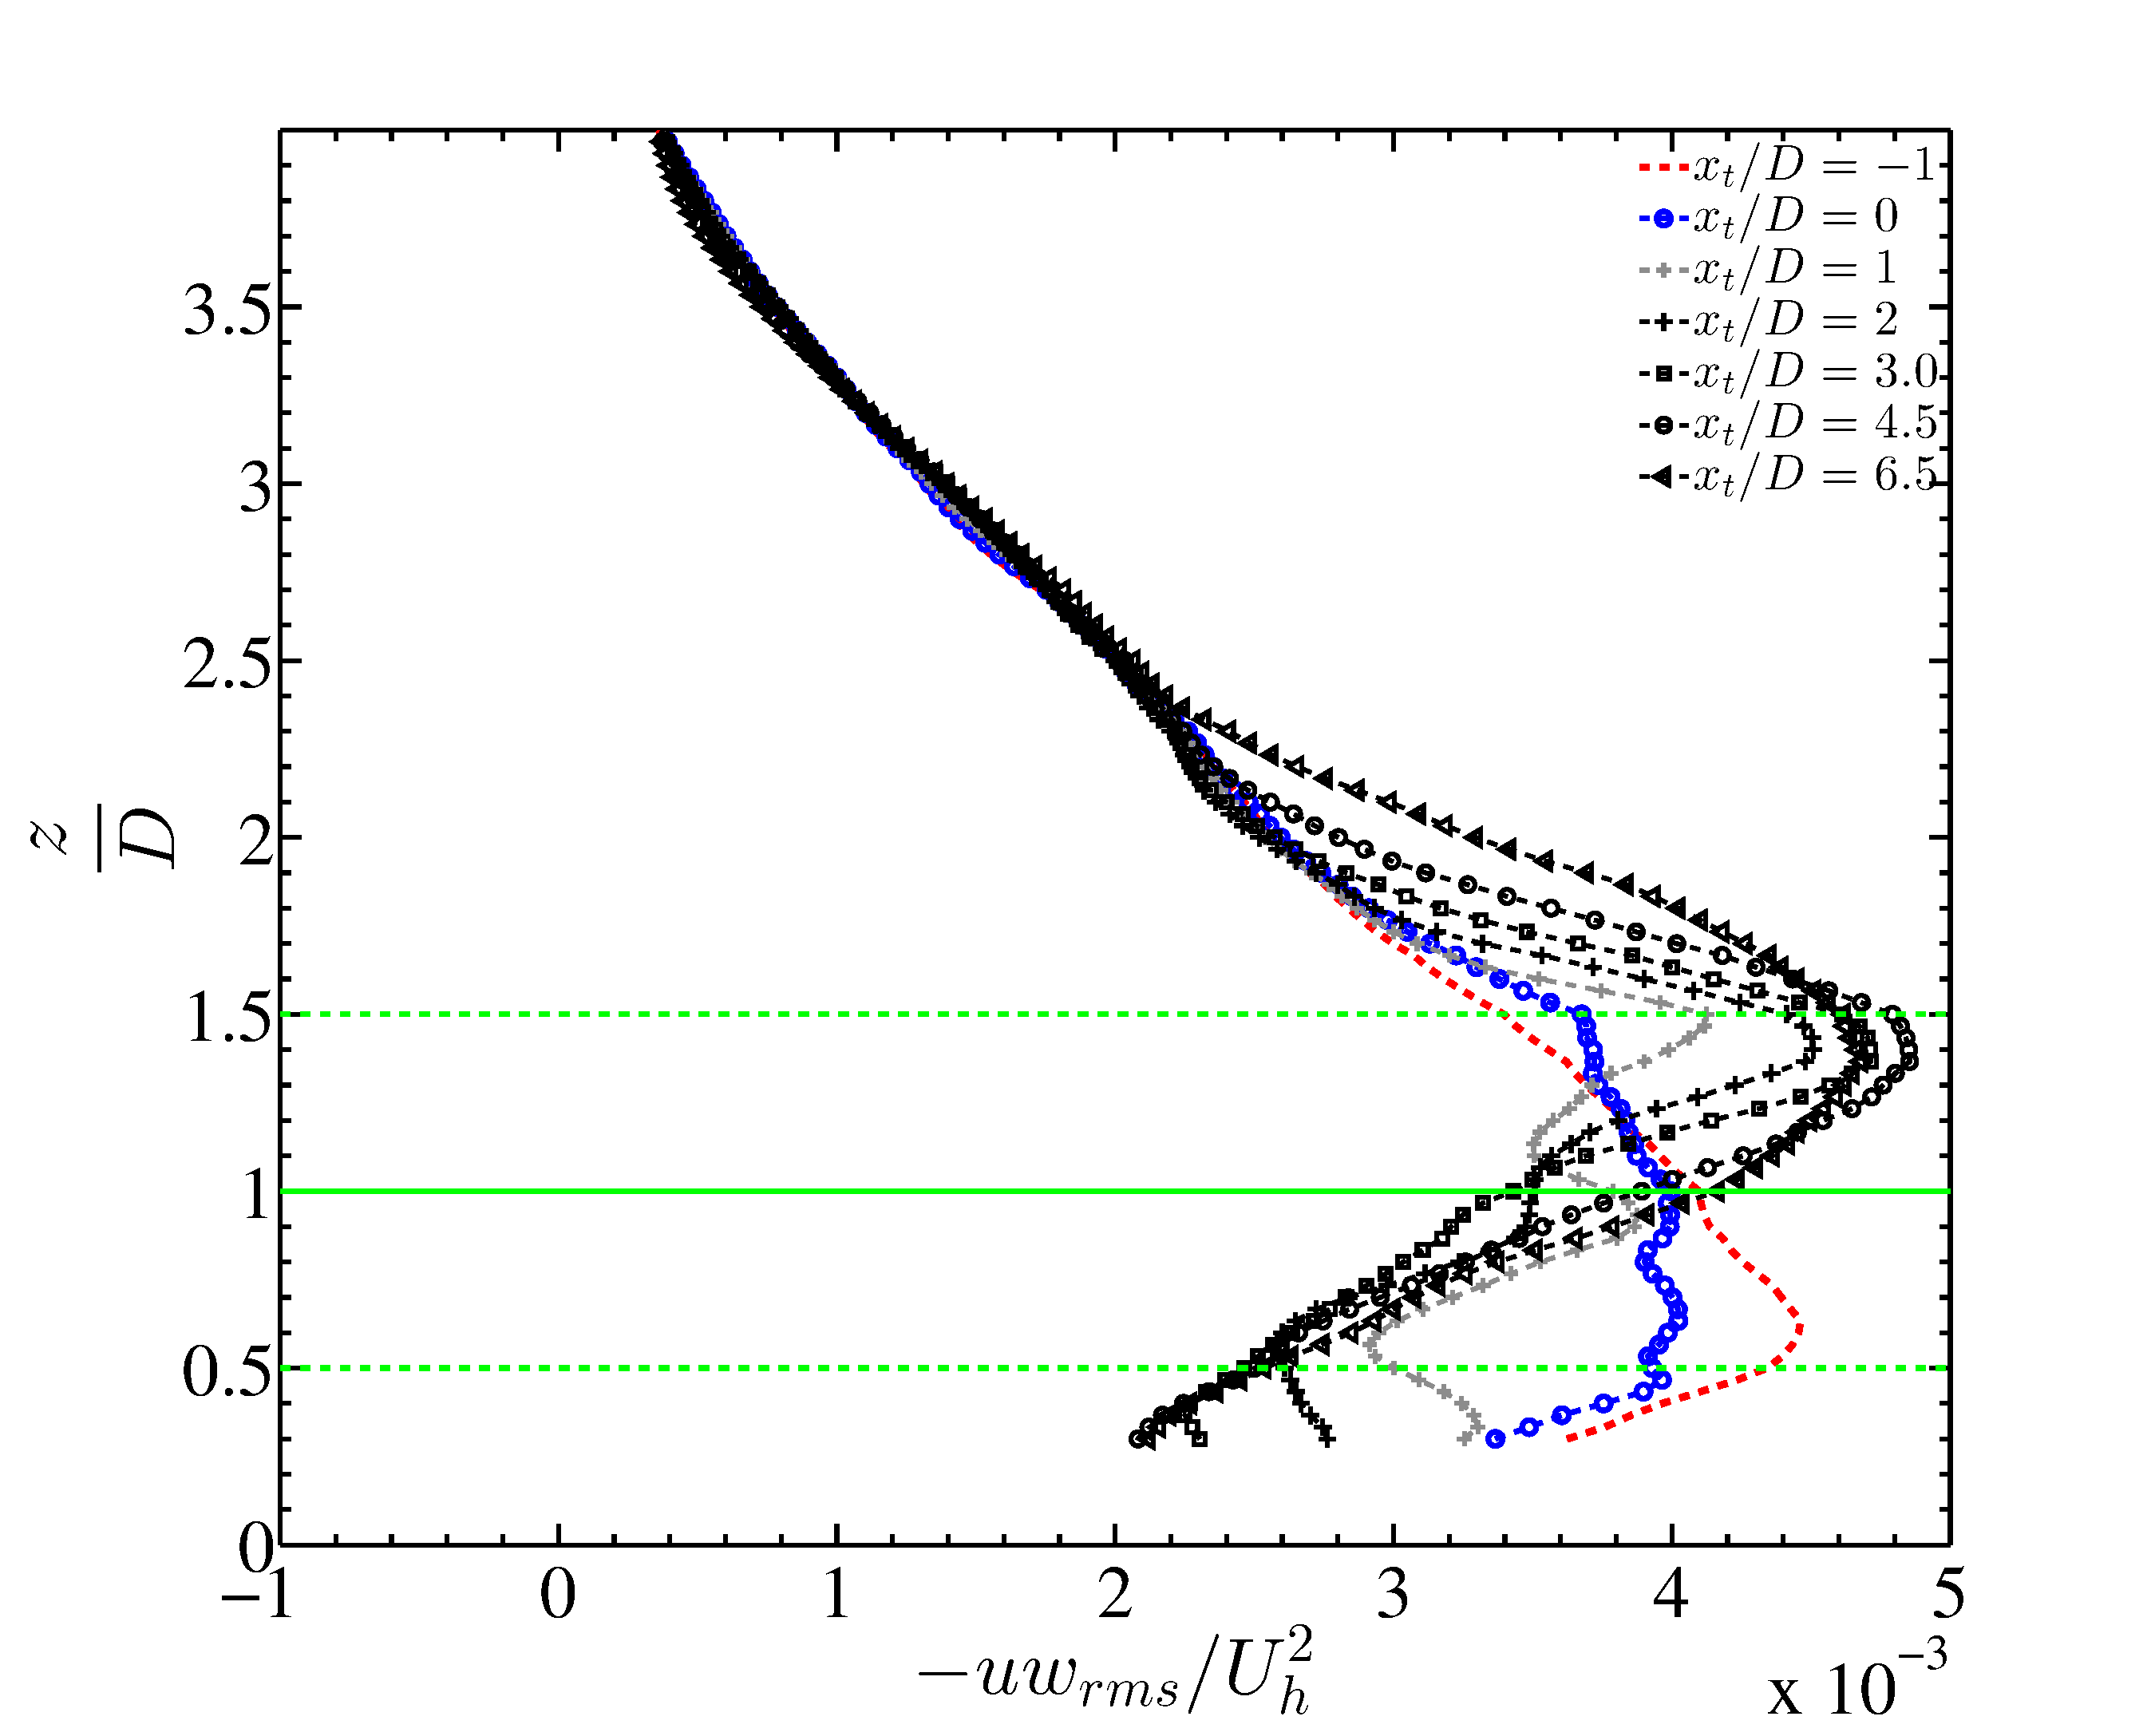
\includegraphics[width = 0.8\linewidth]{stats/shrprof_Npoints_avg.pdf}
\caption[Mean shear stress at $x$ stations 3]{Temporally averaged mean turbulent kinematic shear stress at different streamwise $x$ stations. Profile averaged over the whole spanwise domain.}\label{fig:shrstat3}
\end{figure}




%----------------------------------------------------------------------------------------

\section{Mathematical Tools used in PostProcessing}
\subsection{Helicity}
Helicity is a quadratic invariant of Eulerian equation of fluid motion and can be given as the integral of the dot product of velocity and vorticity vector over the whole flow domain.
\begin{equation}
\mathcal{H} = \int_{\Omega}\pmb{u}\cdot\pmb{\omega}\mathrm{d}V \label{eq:hel1}
\end{equation}
In physical terms it represents the degree of linkage of the vortex lines of flow, conserved when conditions are such that these vortex lines are frozen within the fluid [Moffat].
It is easy to observe that in 3D Navier-Stokes flow, where the diffusion term is negligible for very high Reynolds number flow, the vorticity equation can be written as
\begin{equation}
\frac{D \pmb{\omega}}{D t} = \nabla \times (\pmb{u}\times \pmb{\omega}) \label{eq:link}
\end{equation}
Encapsulated in Equation(~\ref{eq:link}) is the ``frozen field of vorticity " with $D\pmb{\omega}/Dt = 0$, manifesting that curl of $\pmb{u}\times \pmb{\omega}$ is zero. The term $\pmb{u}\times \pmb{\omega}$ is directly not related to helicity but is still important as it forms the genesis of the concept that at times long enough so that the flow-field remains differentiable (singularity in vortices have not formed), and the effect of diffusion is negligibly small, the links/ knots in vortex lines should also persist for such long times. From this concept, we can define, the helicity $\mathcal{H}$ as a degree of knottedness in the vortex lines of the flow or the lack of mirror-symmetry of the flow [Moffat]. \\
It is also meaningful to define the helicity density of flow-field which is simply the dot product of $\pmb{u}$ and $\pmb{\omega}$. It is important to note, that while $\mathcal{H}$ assumes a single scalar value for the whole flow-field, helicity density field $h = \pmb{u}\cdot \pmb{\omega}$ on the other hand is a scalar field and should contain more information in it than the simple value of helicity $\mathcal{H}$. The 3D NS equation with viscous diffusion can be written as 
\begin{equation}
\frac{\partial \pmb{u}}{\partial t} = -\nabla h + (\pmb{u}\times \pmb{\omega}) + \nu \nabla ^{2} \pmb{u}, \ \ \nabla \cdot \pmb{u} = 0 \label{eq:nsh}
\end{equation} 
If we identify some regions within the turbulence field, the helicity density $\pmb{u}\cdot\pmb{\omega}$ is maximal or near maximal, so that $\pmb{u}$ is nearly parallel to $\pm \pmb{\omega}$. Then in such regions the nonlinear term $\pmb{u}\times \pmb{\omega}$ of Equation(~\ref{eq:nsh}) is small, so that a reduction in the nonlinear cascade of energy to smaller scales can be expected. Thus apparently the main effect of helicity in turbulent flow should be to inhibit this (Kolmogorov) cascade; and indeed the flow structures in regions where $\pmb{u}\times \pmb{\omega}$ is near maximal should for this
reason tend to persist coherently in time; they can be thought to be potentially good candidates as the coherent structures of turbulence, about which much has been written [].
In this chapter, we analyse the helicity density field of turbulent flow past the wind turbine arrays to understand the potential coherent structures that play a significant role in the power generation in wind turbines.
\subsection{Lamb Vector Divergence}

\begin{figure}
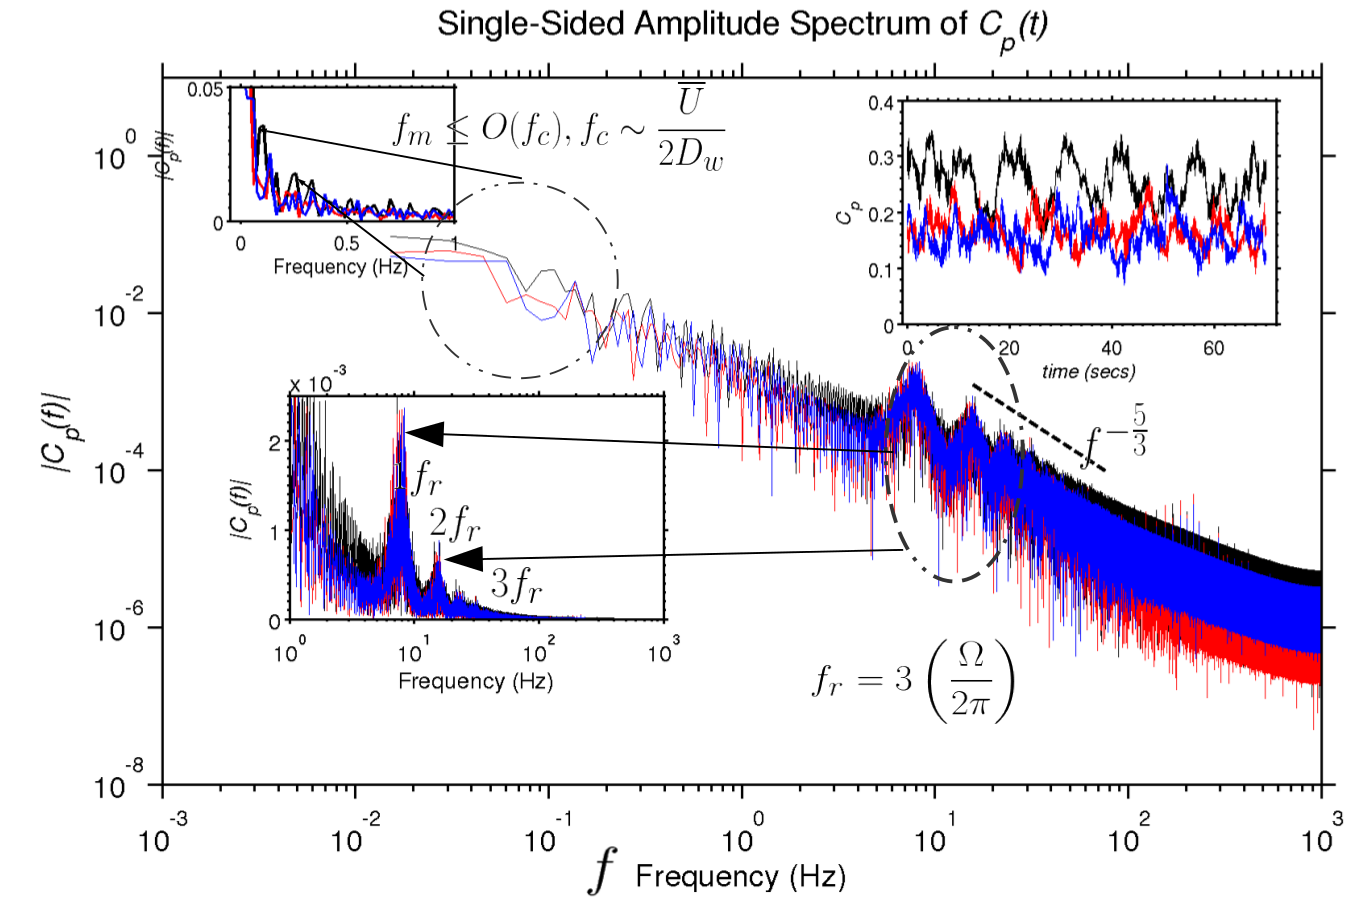
\includegraphics[width = 0.95\linewidth]{Figure/power_2.png}
\caption[Power Spectrum]{Power spectrum in the middle plane of first second and third row in wind turbines.$-5/3$ cascade law of energy and multiple harmonics corresponding to the rotational frequency of turbine blades. } \label{fig:power2}
\end{figure}